\documentclass[11pt, a4paper, logo, copyright]{googledeepmind}

\usepackage[authoryear, sort&compress, round]{natbib}
\bibliographystyle{abbrvnat}

\usepackage[]{mdframed}

\usepackage{dblfloatfix}

\usepackage{amsmath,amsfonts,bm}

\newcommand{\figleft}{{\em (Left)}}
\newcommand{\figcenter}{{\em (Center)}}
\newcommand{\figright}{{\em (Right)}}
\newcommand{\figtop}{{\em (Top)}}
\newcommand{\figbottom}{{\em (Bottom)}}
\newcommand{\captiona}{{\em (a)}}
\newcommand{\captionb}{{\em (b)}}
\newcommand{\captionc}{{\em (c)}}
\newcommand{\captiond}{{\em (d)}}

\newcommand{\newterm}[1]{{\bf #1}}


\def\figref#1{figure~\ref{#1}}
\def\Figref#1{Figure~\ref{#1}}
\def\twofigref#1#2{figures \ref{#1} and \ref{#2}}
\def\quadfigref#1#2#3#4{figures \ref{#1}, \ref{#2}, \ref{#3} and \ref{#4}}
\def\secref#1{section~\ref{#1}}
\def\Secref#1{Section~\ref{#1}}
\def\twosecrefs#1#2{sections \ref{#1} and \ref{#2}}
\def\secrefs#1#2#3{sections \ref{#1}, \ref{#2} and \ref{#3}}
\def\eqref#1{equation~\ref{#1}}
\def\Eqref#1{Equation~\ref{#1}}
\def\plaineqref#1{\ref{#1}}
\def\chapref#1{chapter~\ref{#1}}
\def\Chapref#1{Chapter~\ref{#1}}
\def\rangechapref#1#2{chapters\ref{#1}--\ref{#2}}
\def\algref#1{algorithm~\ref{#1}}
\def\Algref#1{Algorithm~\ref{#1}}
\def\twoalgref#1#2{algorithms \ref{#1} and \ref{#2}}
\def\Twoalgref#1#2{Algorithms \ref{#1} and \ref{#2}}
\def\partref#1{part~\ref{#1}}
\def\Partref#1{Part~\ref{#1}}
\def\twopartref#1#2{parts \ref{#1} and \ref{#2}}

\def\ceil#1{\lceil #1 \rceil}
\def\floor#1{\lfloor #1 \rfloor}
\def\1{\bm{1}}
\newcommand{\train}{\mathcal{D}}
\newcommand{\valid}{\mathcal{D_{\mathrm{valid}}}}
\newcommand{\test}{\mathcal{D_{\mathrm{test}}}}

\def\eps{{\epsilon}}


\def\reta{{\textnormal{$\eta$}}}
\def\ra{{\textnormal{a}}}
\def\rb{{\textnormal{b}}}
\def\rc{{\textnormal{c}}}
\def\rd{{\textnormal{d}}}
\def\re{{\textnormal{e}}}
\def\rf{{\textnormal{f}}}
\def\rg{{\textnormal{g}}}
\def\rh{{\textnormal{h}}}
\def\ri{{\textnormal{i}}}
\def\rj{{\textnormal{j}}}
\def\rk{{\textnormal{k}}}
\def\rl{{\textnormal{l}}}
\def\rn{{\textnormal{n}}}
\def\ro{{\textnormal{o}}}
\def\rp{{\textnormal{p}}}
\def\rq{{\textnormal{q}}}
\def\rr{{\textnormal{r}}}
\def\rs{{\textnormal{s}}}
\def\rt{{\textnormal{t}}}
\def\ru{{\textnormal{u}}}
\def\rv{{\textnormal{v}}}
\def\rw{{\textnormal{w}}}
\def\rx{{\textnormal{x}}}
\def\ry{{\textnormal{y}}}
\def\rz{{\textnormal{z}}}

\def\rvepsilon{{\mathbf{\epsilon}}}
\def\rvtheta{{\mathbf{\theta}}}
\def\rva{{\mathbf{a}}}
\def\rvb{{\mathbf{b}}}
\def\rvc{{\mathbf{c}}}
\def\rvd{{\mathbf{d}}}
\def\rve{{\mathbf{e}}}
\def\rvf{{\mathbf{f}}}
\def\rvg{{\mathbf{g}}}
\def\rvh{{\mathbf{h}}}
\def\rvu{{\mathbf{i}}}
\def\rvj{{\mathbf{j}}}
\def\rvk{{\mathbf{k}}}
\def\rvl{{\mathbf{l}}}
\def\rvm{{\mathbf{m}}}
\def\rvn{{\mathbf{n}}}
\def\rvo{{\mathbf{o}}}
\def\rvp{{\mathbf{p}}}
\def\rvq{{\mathbf{q}}}
\def\rvr{{\mathbf{r}}}
\def\rvs{{\mathbf{s}}}
\def\rvt{{\mathbf{t}}}
\def\rvu{{\mathbf{u}}}
\def\rvv{{\mathbf{v}}}
\def\rvw{{\mathbf{w}}}
\def\rvx{{\mathbf{x}}}
\def\rvy{{\mathbf{y}}}
\def\rvz{{\mathbf{z}}}

\def\erva{{\textnormal{a}}}
\def\ervb{{\textnormal{b}}}
\def\ervc{{\textnormal{c}}}
\def\ervd{{\textnormal{d}}}
\def\erve{{\textnormal{e}}}
\def\ervf{{\textnormal{f}}}
\def\ervg{{\textnormal{g}}}
\def\ervh{{\textnormal{h}}}
\def\ervi{{\textnormal{i}}}
\def\ervj{{\textnormal{j}}}
\def\ervk{{\textnormal{k}}}
\def\ervl{{\textnormal{l}}}
\def\ervm{{\textnormal{m}}}
\def\ervn{{\textnormal{n}}}
\def\ervo{{\textnormal{o}}}
\def\ervp{{\textnormal{p}}}
\def\ervq{{\textnormal{q}}}
\def\ervr{{\textnormal{r}}}
\def\ervs{{\textnormal{s}}}
\def\ervt{{\textnormal{t}}}
\def\ervu{{\textnormal{u}}}
\def\ervv{{\textnormal{v}}}
\def\ervw{{\textnormal{w}}}
\def\ervx{{\textnormal{x}}}
\def\ervy{{\textnormal{y}}}
\def\ervz{{\textnormal{z}}}

\def\rmA{{\mathbf{A}}}
\def\rmB{{\mathbf{B}}}
\def\rmC{{\mathbf{C}}}
\def\rmD{{\mathbf{D}}}
\def\rmE{{\mathbf{E}}}
\def\rmF{{\mathbf{F}}}
\def\rmG{{\mathbf{G}}}
\def\rmH{{\mathbf{H}}}
\def\rmI{{\mathbf{I}}}
\def\rmJ{{\mathbf{J}}}
\def\rmK{{\mathbf{K}}}
\def\rmL{{\mathbf{L}}}
\def\rmM{{\mathbf{M}}}
\def\rmN{{\mathbf{N}}}
\def\rmO{{\mathbf{O}}}
\def\rmP{{\mathbf{P}}}
\def\rmQ{{\mathbf{Q}}}
\def\rmR{{\mathbf{R}}}
\def\rmS{{\mathbf{S}}}
\def\rmT{{\mathbf{T}}}
\def\rmU{{\mathbf{U}}}
\def\rmV{{\mathbf{V}}}
\def\rmW{{\mathbf{W}}}
\def\rmX{{\mathbf{X}}}
\def\rmY{{\mathbf{Y}}}
\def\rmZ{{\mathbf{Z}}}

\def\ermA{{\textnormal{A}}}
\def\ermB{{\textnormal{B}}}
\def\ermC{{\textnormal{C}}}
\def\ermD{{\textnormal{D}}}
\def\ermE{{\textnormal{E}}}
\def\ermF{{\textnormal{F}}}
\def\ermG{{\textnormal{G}}}
\def\ermH{{\textnormal{H}}}
\def\ermI{{\textnormal{I}}}
\def\ermJ{{\textnormal{J}}}
\def\ermK{{\textnormal{K}}}
\def\ermL{{\textnormal{L}}}
\def\ermM{{\textnormal{M}}}
\def\ermN{{\textnormal{N}}}
\def\ermO{{\textnormal{O}}}
\def\ermP{{\textnormal{P}}}
\def\ermQ{{\textnormal{Q}}}
\def\ermR{{\textnormal{R}}}
\def\ermS{{\textnormal{S}}}
\def\ermT{{\textnormal{T}}}
\def\ermU{{\textnormal{U}}}
\def\ermV{{\textnormal{V}}}
\def\ermW{{\textnormal{W}}}
\def\ermX{{\textnormal{X}}}
\def\ermY{{\textnormal{Y}}}
\def\ermZ{{\textnormal{Z}}}

\def\vzero{{\bm{0}}}
\def\vone{{\bm{1}}}
\def\vmu{{\bm{\mu}}}
\def\vtheta{{\bm{\theta}}}
\def\va{{\bm{a}}}
\def\vb{{\bm{b}}}
\def\vc{{\bm{c}}}
\def\vd{{\bm{d}}}
\def\ve{{\bm{e}}}
\def\vf{{\bm{f}}}
\def\vg{{\bm{g}}}
\def\vh{{\bm{h}}}
\def\vi{{\bm{i}}}
\def\vj{{\bm{j}}}
\def\vk{{\bm{k}}}
\def\vl{{\bm{l}}}
\def\vm{{\bm{m}}}
\def\vn{{\bm{n}}}
\def\vo{{\bm{o}}}
\def\vp{{\bm{p}}}
\def\vq{{\bm{q}}}
\def\vr{{\bm{r}}}
\def\vs{{\bm{s}}}
\def\vt{{\bm{t}}}
\def\vu{{\bm{u}}}
\def\vv{{\bm{v}}}
\def\vw{{\bm{w}}}
\def\vx{{\bm{x}}}
\def\vy{{\bm{y}}}
\def\vz{{\bm{z}}}

\def\evalpha{{\alpha}}
\def\evbeta{{\beta}}
\def\evepsilon{{\epsilon}}
\def\evlambda{{\lambda}}
\def\evomega{{\omega}}
\def\evmu{{\mu}}
\def\evpsi{{\psi}}
\def\evsigma{{\sigma}}
\def\evtheta{{\theta}}
\def\eva{{a}}
\def\evb{{b}}
\def\evc{{c}}
\def\evd{{d}}
\def\eve{{e}}
\def\evf{{f}}
\def\evg{{g}}
\def\evh{{h}}
\def\evi{{i}}
\def\evj{{j}}
\def\evk{{k}}
\def\evl{{l}}
\def\evm{{m}}
\def\evn{{n}}
\def\evo{{o}}
\def\evp{{p}}
\def\evq{{q}}
\def\evr{{r}}
\def\evs{{s}}
\def\evt{{t}}
\def\evu{{u}}
\def\evv{{v}}
\def\evw{{w}}
\def\evx{{x}}
\def\evy{{y}}
\def\evz{{z}}

\def\mA{{\bm{A}}}
\def\mB{{\bm{B}}}
\def\mC{{\bm{C}}}
\def\mD{{\bm{D}}}
\def\mE{{\bm{E}}}
\def\mF{{\bm{F}}}
\def\mG{{\bm{G}}}
\def\mH{{\bm{H}}}
\def\mI{{\bm{I}}}
\def\mJ{{\bm{J}}}
\def\mK{{\bm{K}}}
\def\mL{{\bm{L}}}
\def\mM{{\bm{M}}}
\def\mN{{\bm{N}}}
\def\mO{{\bm{O}}}
\def\mP{{\bm{P}}}
\def\mQ{{\bm{Q}}}
\def\mR{{\bm{R}}}
\def\mS{{\bm{S}}}
\def\mT{{\bm{T}}}
\def\mU{{\bm{U}}}
\def\mV{{\bm{V}}}
\def\mW{{\bm{W}}}
\def\mX{{\bm{X}}}
\def\mY{{\bm{Y}}}
\def\mZ{{\bm{Z}}}
\def\mBeta{{\bm{\beta}}}
\def\mPhi{{\bm{\Phi}}}
\def\mLambda{{\bm{\Lambda}}}
\def\mSigma{{\bm{\Sigma}}}

\DeclareMathAlphabet{\mathsfit}{\encodingdefault}{\sfdefault}{m}{sl}
\SetMathAlphabet{\mathsfit}{bold}{\encodingdefault}{\sfdefault}{bx}{n}
\newcommand{\tens}[1]{\bm{\mathsfit{#1}}}
\def\tA{{\tens{A}}}
\def\tB{{\tens{B}}}
\def\tC{{\tens{C}}}
\def\tD{{\tens{D}}}
\def\tE{{\tens{E}}}
\def\tF{{\tens{F}}}
\def\tG{{\tens{G}}}
\def\tH{{\tens{H}}}
\def\tI{{\tens{I}}}
\def\tJ{{\tens{J}}}
\def\tK{{\tens{K}}}
\def\tL{{\tens{L}}}
\def\tM{{\tens{M}}}
\def\tN{{\tens{N}}}
\def\tO{{\tens{O}}}
\def\tP{{\tens{P}}}
\def\tQ{{\tens{Q}}}
\def\tR{{\tens{R}}}
\def\tS{{\tens{S}}}
\def\tT{{\tens{T}}}
\def\tU{{\tens{U}}}
\def\tV{{\tens{V}}}
\def\tW{{\tens{W}}}
\def\tX{{\tens{X}}}
\def\tY{{\tens{Y}}}
\def\tZ{{\tens{Z}}}


\def\gA{{\mathcal{A}}}
\def\gB{{\mathcal{B}}}
\def\gC{{\mathcal{C}}}
\def\gD{{\mathcal{D}}}
\def\gE{{\mathcal{E}}}
\def\gF{{\mathcal{F}}}
\def\gG{{\mathcal{G}}}
\def\gH{{\mathcal{H}}}
\def\gI{{\mathcal{I}}}
\def\gJ{{\mathcal{J}}}
\def\gK{{\mathcal{K}}}
\def\gL{{\mathcal{L}}}
\def\gM{{\mathcal{M}}}
\def\gN{{\mathcal{N}}}
\def\gO{{\mathcal{O}}}
\def\gP{{\mathcal{P}}}
\def\gQ{{\mathcal{Q}}}
\def\gR{{\mathcal{R}}}
\def\gS{{\mathcal{S}}}
\def\gT{{\mathcal{T}}}
\def\gU{{\mathcal{U}}}
\def\gV{{\mathcal{V}}}
\def\gW{{\mathcal{W}}}
\def\gX{{\mathcal{X}}}
\def\gY{{\mathcal{Y}}}
\def\gZ{{\mathcal{Z}}}

\def\sA{{\mathbb{A}}}
\def\sB{{\mathbb{B}}}
\def\sC{{\mathbb{C}}}
\def\sD{{\mathbb{D}}}
\def\sF{{\mathbb{F}}}
\def\sG{{\mathbb{G}}}
\def\sH{{\mathbb{H}}}
\def\sI{{\mathbb{I}}}
\def\sJ{{\mathbb{J}}}
\def\sK{{\mathbb{K}}}
\def\sL{{\mathbb{L}}}
\def\sM{{\mathbb{M}}}
\def\sN{{\mathbb{N}}}
\def\sO{{\mathbb{O}}}
\def\sP{{\mathbb{P}}}
\def\sQ{{\mathbb{Q}}}
\def\sR{{\mathbb{R}}}
\def\sS{{\mathbb{S}}}
\def\sT{{\mathbb{T}}}
\def\sU{{\mathbb{U}}}
\def\sV{{\mathbb{V}}}
\def\sW{{\mathbb{W}}}
\def\sX{{\mathbb{X}}}
\def\sY{{\mathbb{Y}}}
\def\sZ{{\mathbb{Z}}}

\def\emLambda{{\Lambda}}
\def\emA{{A}}
\def\emB{{B}}
\def\emC{{C}}
\def\emD{{D}}
\def\emE{{E}}
\def\emF{{F}}
\def\emG{{G}}
\def\emH{{H}}
\def\emI{{I}}
\def\emJ{{J}}
\def\emK{{K}}
\def\emL{{L}}
\def\emM{{M}}
\def\emN{{N}}
\def\emO{{O}}
\def\emP{{P}}
\def\emQ{{Q}}
\def\emR{{R}}
\def\emS{{S}}
\def\emT{{T}}
\def\emU{{U}}
\def\emV{{V}}
\def\emW{{W}}
\def\emX{{X}}
\def\emY{{Y}}
\def\emZ{{Z}}
\def\emSigma{{\Sigma}}

\newcommand{\etens}[1]{\mathsfit{#1}}
\def\etLambda{{\etens{\Lambda}}}
\def\etA{{\etens{A}}}
\def\etB{{\etens{B}}}
\def\etC{{\etens{C}}}
\def\etD{{\etens{D}}}
\def\etE{{\etens{E}}}
\def\etF{{\etens{F}}}
\def\etG{{\etens{G}}}
\def\etH{{\etens{H}}}
\def\etI{{\etens{I}}}
\def\etJ{{\etens{J}}}
\def\etK{{\etens{K}}}
\def\etL{{\etens{L}}}
\def\etM{{\etens{M}}}
\def\etN{{\etens{N}}}
\def\etO{{\etens{O}}}
\def\etP{{\etens{P}}}
\def\etQ{{\etens{Q}}}
\def\etR{{\etens{R}}}
\def\etS{{\etens{S}}}
\def\etT{{\etens{T}}}
\def\etU{{\etens{U}}}
\def\etV{{\etens{V}}}
\def\etW{{\etens{W}}}
\def\etX{{\etens{X}}}
\def\etY{{\etens{Y}}}
\def\etZ{{\etens{Z}}}

\newcommand{\pdata}{p_{\rm{data}}}
\newcommand{\ptrain}{\hat{p}_{\rm{data}}}
\newcommand{\Ptrain}{\hat{P}_{\rm{data}}}
\newcommand{\pmodel}{p_{\rm{model}}}
\newcommand{\Pmodel}{P_{\rm{model}}}
\newcommand{\ptildemodel}{\tilde{p}_{\rm{model}}}
\newcommand{\pencode}{p_{\rm{encoder}}}
\newcommand{\pdecode}{p_{\rm{decoder}}}
\newcommand{\precons}{p_{\rm{reconstruct}}}

\newcommand{\laplace}{\mathrm{Laplace}} %

\newcommand{\E}{\mathbb{E}}
\newcommand{\Ls}{\mathcal{L}}
\newcommand{\R}{\mathbb{R}}
\newcommand{\emp}{\tilde{p}}
\newcommand{\lr}{\alpha}
\newcommand{\reg}{\lambda}
\newcommand{\rect}{\mathrm{rectifier}}
\newcommand{\softmax}{\mathrm{softmax}}
\newcommand{\sigmoid}{\sigma}
\newcommand{\softplus}{\zeta}
\newcommand{\KL}{D_{\mathrm{KL}}}
\newcommand{\Var}{\mathrm{Var}}
\newcommand{\standarderror}{\mathrm{SE}}
\newcommand{\Cov}{\mathrm{Cov}}
\newcommand{\normlzero}{L^0}
\newcommand{\normlone}{L^1}
\newcommand{\normltwo}{L^2}
\newcommand{\normlp}{L^p}
\newcommand{\normmax}{L^\infty}

\newcommand{\parents}{Pa} %

\DeclareMathOperator*{\argmax}{arg\,max}
\DeclareMathOperator*{\argmin}{arg\,min}

\DeclareMathOperator{\sign}{sign}
\DeclareMathOperator{\Tr}{Tr}
\let\ab\allowbreak

\usepackage{listings}
\usepackage{hyperref}
\usepackage{url}
\usepackage{graphicx}
\usepackage{amsmath} %
\usepackage{mathrsfs} %
\usepackage{etoolbox}
\usepackage{cleveref}
\usepackage{tcolorbox}
\usepackage{colortbl}
\usepackage{booktabs}       %
\usepackage{amsfonts}       %
\usepackage{nicefrac}       %
\usepackage{microtype}      %
\usepackage{subcaption}
\usepackage{algorithm}
\usepackage{algorithmic}
\usepackage{multirow}
\usepackage{subcaption}

\usepackage{booktabs} %
\usepackage{enumitem}%
\setlist[itemize]{noitemsep, topsep=0pt}
\usepackage{enumitem,kantlipsum}

\newlength\savewidth\newcommand\shline{\noalign{\global\savewidth\arrayrulewidth
  \global\arrayrulewidth 1pt}\hline\noalign{\global\arrayrulewidth\savewidth}}
\newcommand{\tablestyle}[2]{\setlength{\tabcolsep}{#1}\renewcommand{\arraystretch}{#2}\centering\footnotesize}
\definecolor{baselinecolor}{HTML}{d6eaf8}
\newcommand{\baseline}[1]{\cellcolor{baselinecolor}{#1}}
\definecolor{mygray}{gray}{0.4}
\newenvironment{mytiny}{\color{mygray}\small}{}

\AtBeginEnvironment{tcolorbox}{\tiny}


\newcount\Comments  %
\Comments=0   %
\usepackage{color}
\definecolor{darkred}{rgb}{0.9,0,0}
\definecolor{darkgreen}{rgb}{0,0.5,0}
\definecolor{darkblue}{rgb}{0,0,0.7}
\definecolor{purple}{rgb}{.6, 0,.6}
\definecolor{orange}{rgb}{1.0,0.64,0}
\newcommand{\kibitz}[2]{\ifnum\Comments=1\textcolor{#1}{#2}\fi}
\newcommand{\zw}[1]{\kibitz{red}      {[ZW: #1]}}
\newcommand{\bk}[1]{\kibitz{blue}      {[BK: #1]}}

\newcommand{\nitkan}[1]{\kibitz{blue}      {[NK: #1]}}
\newcommand{\wenjun}[1]{\kibitz{violet}      {[wenjun: #1]}}

\newcommand{\meera}[1]{\kibitz{orange}      {[meera: #1]}}

\title{Proactive Agents for Multi-Turn Text-to-Image Generation Under Uncertainty}
\correspondingauthor{Zi Wang (wangzi@google.com). Contributions and emails of all authors in \Cref{sec:authors}.}


\reportnumber{001} %

\renewcommand{\today}{2024-12}

\author[*,1]{Meera Hahn}
\author[2]{Wenjun Zeng}
\author[3]{Nithish Kannen}
\author[4]{Rich Galt}
\author[4]{Kartikeya Badola}
\author[2]{Been Kim}
\author[*,5]{Zi Wang}

\affil[*]{Equal contributions}
\affil[1]{Google DeepMind, Atlanta, GA, USA}
\affil[2]{Google DeepMind, Seattle, WA, USA}
\affil[3]{Google DeepMind, Bangalore, India}
\affil[4]{Google DeepMind, London, UK}
\affil[5]{Google DeepMind, Cambridge, MA, USA}

\begin{abstract}
\vspace{-1em}
\begin{abstract}
There is a widely-spread claim that GANs are difficult to train, and GAN architectures in the literature are littered with empirical tricks. We provide evidence against this claim and build a modern GAN baseline in a more principled manner. First, we derive a well-behaved regularized relativistic GAN loss that addresses issues of mode dropping and non-convergence that were previously tackled via a bag of ad-hoc tricks. We analyze our loss mathematically and prove that it admits local convergence guarantees, unlike most existing relativistic losses. Second, this loss allows us to discard all ad-hoc tricks and replace outdated backbones used in common GANs with modern architectures. Using StyleGAN2 as an example, we present a roadmap of simplification and modernization that results in a new minimalist baseline---\modelName (``Re-GAN''). Despite being simple, our approach surpasses StyleGAN2 on FFHQ, ImageNet, CIFAR, and Stacked MNIST datasets, and compares favorably against state-of-the-art GANs and diffusion models.\\
Code: \href{https://www.github.com/brownvc/R3GAN}{https://www.github.com/brownvc/R3GAN}
\end{abstract}
\end{abstract}


\begin{document}

\maketitle

\section{Introduction}
\label{sec:intro}


Transformers, in particular decoder-only models (e.g.\ GPT~\citep{brown2020language}, Llama~\citep{touvron2023llama}) which process input sequences in a causal fashion, are one of the main drivers of modern deep learning's success.
Numerous approaches attempt to approximate the core attention layer to address its efficiency issues~\citep{tay2022efficient}, such as scaling quadratically in sequence length during training and requiring a cache of size linear in sequence length during autoregressive generation.
In parallel, a class of alternative sequence models, structured state-space models (SSMs), have emerged with linear scaling in sequence length during training and constant state size during generation.
They show strong performance on long-range tasks (e.g. S4~\citep{gu2022efficiently}) and recently matched or beat Transformers on language modeling (e.g. Mamba \citep{gu2023mamba}) at small to moderate scale.
However, the development of SSMs have appeared disjoint from the community's collective effort to improve Transformers, such as understanding them theoretically as well as optimizing them on modern hardware.
As a result, it is more difficult to understand and experiment with SSMs compared to Transformers, and it remains challenging to train SSMs as efficiently as Transformers from both an algorithmic and systems perspective.


Our main goal is to develop a rich body of theoretical connections between structured SSMs and variants of attention.
This will allow us to transfer algorithmic and systems optimizations originally developed for Transformers to SSMs, towards the goal of building foundation models that perform better than Transformers while scaling more efficiently in sequence length.
A milestone contribution in this direction was the \textbf{Linear Attention (LA)} framework \citep{katharopoulos2020transformers},
which derived a connection between autoregressive attention and linear RNNs
by showing the equivalence between ``dual forms'' of quadratic kernelized attention and a particular linear recurrence.
This duality allows new capabilities such as the ability to have both efficient parallelizable training and efficient autoregressive inference.
In the same spirit, this paper provides multiple viewpoints connecting linear-complexity SSMs with quadratic-complexity forms to combine the strengths of SSMs and attention.%
\footnote{Technically speaking, these connections only relate to certain flavors of attention; the title of this paper is an homage to \citet{katharopoulos2020transformers} which first showed that ``Transformers are RNNs''.}

\iftoggle{arxiv}{
\begin{wrapfigure}{R}{0.48\linewidth}
  \begin{center}
    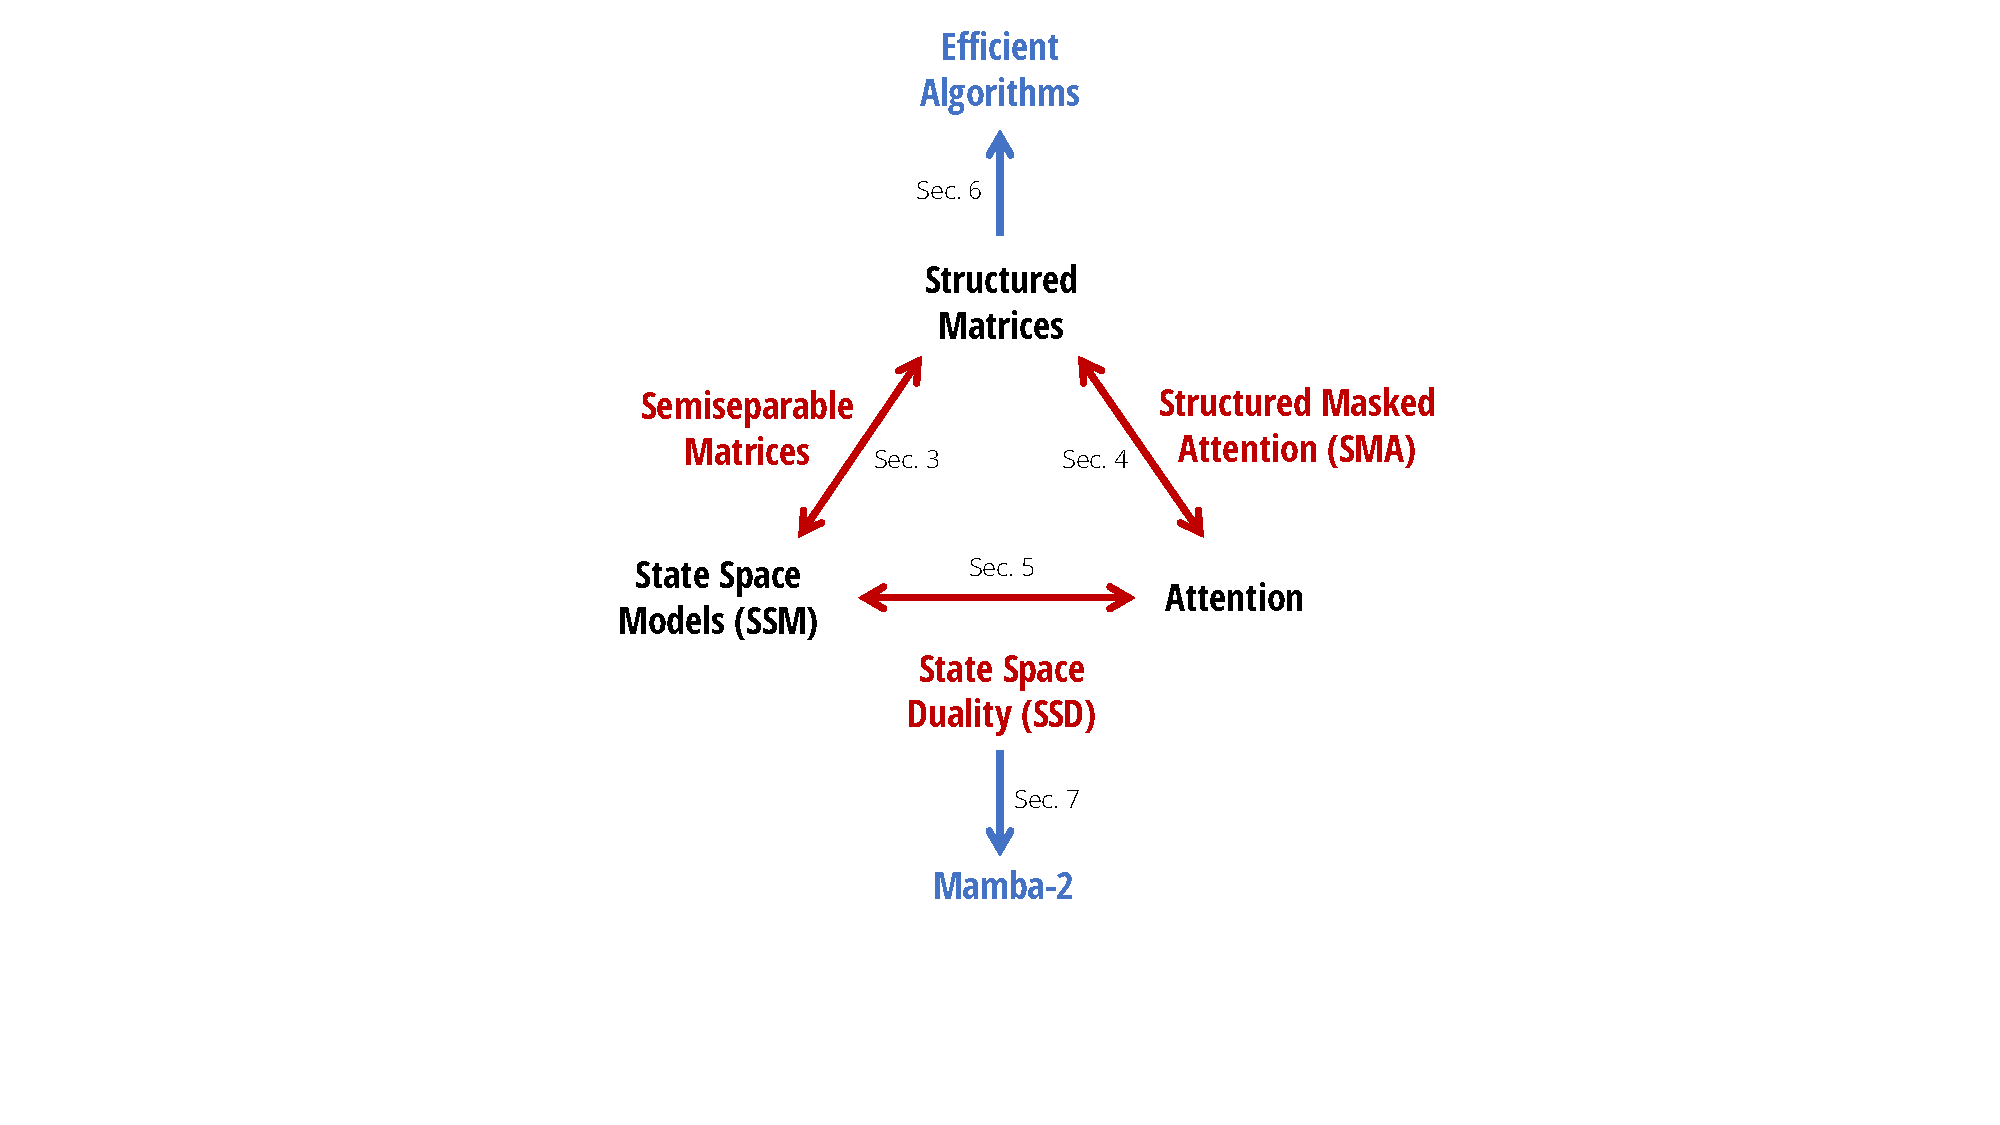
\includegraphics[width=\linewidth]{fig/ssd_roadmap.pdf}
  \end{center}
  \caption{
    (\textbf{Structured State-Space Duality}.)
    This paper fleshes out the relationship between state space models and attention through the bridge of structured matrices.
  }
  \label{fig:roadmap}
\end{wrapfigure}
}{}

\para{State Space Duality.}
Our framework connecting structured SSMs and variants of attention, which we call \textbf{structured state space duality} (SSD),
is made through the abstractions of \textbf{structured matrices}:
matrices with subquadratic parameters and multiplication complexity.
We develop two broad frameworks for representing sequence models, one as matrix transformations and one as tensor contractions, which each reveal different perspectives of the duality.
Our technical contributions include:
\begin{itemize}[leftmargin=*,itemsep=0pt,topsep=0pt]
  \item We show an equivalence between state space models and a well-studied family of structured matrices called \textbf{semiseparable matrices}\iftoggle{arxiv}{ (\cref{sec:ssm})}{}.
    This connection is at the heart our framework, revealing new properties and algorithms for SSMs. A central message of this paper is that \emph{different methods of computing state space models can be reframed as various matrix multiplication algorithms on structured matrices}.
  \item We significantly improve the theory of linear attention~\citep{katharopoulos2020transformers}.
    We first provide an incisive proof of its recurrent form through the language of tensor contractions, and then generalize it to a new family of \textbf{structured masked attention (SMA)}\iftoggle{arxiv}{ (\cref{sec:attention})}{}.
  \item We connect SSMs and SMA, showing that they have a large intersection that are duals of each other, possessing both SSM-like linear and attention-like quadratic forms\iftoggle{arxiv}{ (\cref{sec:ssd})}{}.
    \iftoggle{arxiv}{We also prove that any kernel attention method possessing a fast recurrent form must be an SSM.}{}
\end{itemize}


Beyond its intrinsic theoretical value, our framework opens up a broad set of directions for understanding and improving sequence models.

\para{Efficient Algorithms.}
First and most importantly, our framework exposes new efficient and easily-implementable algorithms for computing SSMs\iftoggle{arxiv}{ (\cref{sec:efficient})}{}.
We introduce a new \textbf{SSD algorithm}, based on block decompositions of semiseparable matrices, that takes advantage of both the linear SSM recurrence and quadratic dual form, obtaining optimal tradeoffs on all main efficiency axes (e.g. training and inference compute, memory usage, and ability to leverage matrix multiplication units on modern hardware).
A dedicated implementation of SSD is $2-8\times$ faster than the optimized selective scan implementation of Mamba, while simultaneously allowing for much larger recurrent state sizes ($8\times$ the size of Mamba or even higher, with minimal slowdown).
SSD is highly competitive with optimized implementations of softmax attention (FlashAttention-2~\citep{dao2023flashattention2}), crossing over at sequence length 2K and 6$\times$ faster at sequence length 16K.


\iftoggle{arxiv}{
\para{Architecture Design.}
One major obstacle to adopting new architectures such as SSMs is the ecosystem tailored to Transformers, such as hardware-efficient optimization and parallelism techniques for large-scale training.
Our framework allows using established conventions and techniques for attention to build a vocabulary of architecture design choices for SSMs, and further improve them (\cref{sec:architecture}).
For example, we introduce the analog of heads from multi-head attention (MHA) to SSMs.
We show that the Mamba architecture is a \textbf{multi-input SSM (MIS)} that turns out to be analogous to \textbf{multi-value attention (MVA)}, and compare other variants of Mamba with different head structures.

We also use these ideas to make slight modifications to the Mamba block, which allows tensor parallelism to be implemented (e.g. in the style of Megatron~\citep{shoeybi2019megatron}).
The main ideas include introducing grouped-value attention (GVA) head structure, and moving all data-dependent projections to occur in parallel at the beginning of the block.


}{
  \para{Mamba-2.}
  Additionally, inspired by the connection between SSMs and Transformers, we slightly modify the neural network architecture of Mamba by moving all data-dependent projections to occur in parallel at the beginning of the block. %
}
The combination of the modified parallel Mamba block, together with using SSD as the inner SSM layer, results in the \textbf{Mamba-2} architecture.
We investigate Chinchilla scaling laws for Mamba-2 in the same setting as Mamba, finding that it Pareto dominates Mamba and Transformer++ in both perplexity and wall-clock time.
We additionally train a family of Mamba-2 models at varying sizes on the Pile, showing that it matches or outperforms Mamba and open source Transformers on standard downstream evaluations.
For example, Mamba-2 with 2.7B parameters trained on 300B tokens on the Pile outperforms Mamba-2.8B, Pythia-2.8B and even Pythia-6.9B trained on the same dataset.

\iftoggle{arxiv}{
\paragraph{Systems Optimizations.}
The SSD framework connects SSMs and Transformers, allowing us to leverage a rich body of work on systems optimizations developed for Transformers~(\cref{sec:systems}).
\begin{itemize}[leftmargin=*,itemsep=0pt,topsep=0pt]
  \item For example, Tensor Parallelism (TP) is an important model parallelism technique to train large Transformer models by splitting each layer across GPUs on the same node.
    We design Mamba-2 to be TP-friendly, reducing the number of synchronization point per block by half.
  \item For very long sequences whose activations do not fit on one device, sequence parallelism has been developed for the attention blocks.
    We describe how to train SSMs in general and Mamba-2 in particular with sequence parallelism, by passing the recurrent states between devices.
  \item For finetuning with examples of different lengths, for best efficiency, Transformer requires sophisticated techniques to remove padding tokens and perform attention on variable length sequences.
    We show how Mamba-2 can be trained with variable sequence lengths efficiently, requiring no padding tokens.
\end{itemize}
}{}

\cref{sec:experiments} empirically validates Mamba-2 on language modeling, training efficiency, and a difficult multi-query associative recall task~\citep{arora2024simple}.
Finally, in \cref{sec:related}, we provide an extended related work and discuss potential research directions opened up by our framework.

Model code and pre-trained checkpoints are open-sourced at \url{https://github.com/state-spaces/mamba}.







\section{Related work}
\label{sec:related}

\nitkan{Maybe adding paragraph headers here could help with the readability. }
From the very outset of \textbf{artificial intelligence}, a core challenge has been to develop intelligent agents capable of representing knowledge and taking actions to acquire knowledge necessary for achieving their goals~\citep{McCHay69, minsky1974framework, moore1985formal, nilsson2009quest, russell2016artificial}. Our work is an attempt to address this challenge for intelligent T2I agents.%

In \textbf{machine learning and statistics}, efficient data acquisition has been extensively studied for many problems, including active learning~\citep{cohn1996active, settles.tr09, houlsby2011bayesian, gal2017deep, ren2021survey, wang2018active}, Bayesian optimization~\citep{garnett2023bayesian, kushner1964, mockus1974,auer2002b, srinivas2009gaussian, hennig2012, wang2017maxvalue,  wang2024pre}, reinforcement learning~\citep{kaelbling1996reinforcement, ghavamzadeh2015bayesian, sutton2018reinforcement} and experimental design~\citep{ chaloner1995bayesian, kirk2009experimental}. %
We reckon that T2I agents should also be capable of actively seeking important information from human users to quickly reduce uncertainty~\citep{wang2024gaussian} and generate satisfying images. In \S\ref{ssec:implementation}, we detail the implementation of action selection strategies for our T2I agents.



In \textbf{human-computer interaction}, researchers have been extensively studying how to best enable Human-AI interaction especially from user experience perspectives~\citep{norman1994might, hook2000steps, amershi2019guidelines, cai2019human, viegas2023system, chen2024designing, yang2020re, kim2023help}. Interface design for AI is becoming increasingly challenging due to the lack of transparency~\citep{viegas2023system, chen2024designing}, uncertainty about AI capability and complex outputs~\citep{yang2020re}. We aim to build user-friendly agents, and an indispensable component is their interface to enable them to effectively act and observe, as detailed in \S\ref{app:interface}.

\textbf{Interpretebaility.} Surfacing an agent's belief overlaps with interpretability as both aim to understand model or agent's internal. Some methods leverage LLM's natural language interface to surface their reasoning (e.g., chain of thought \citep{wei2023chainofthoughtpromptingelicitsreasoning}), sometime interactively \citep{wang2024llmcheckupconversationalexaminationlarge}. While these approaches make accessible explanations, whether the explanations represent truth has been questioned \citep{lanham2023measuringfaithfulnesschainofthoughtreasoning, wei2023largerlanguagemodelsincontext, chen2023modelsexplainthemselvescounterfactual}. Some studies indicate explanations generated by the LLMs may not entail the models’ predictions nor be factually grounded in the input, even on simple tasks with extractive explanations \citep{ye2022unreliabilityexplanationsfewshotprompting}. In this work, the belief graph does not correspond to the distribution over outputs of the T2I \emph{model} itself conditioned on the underspecified prompt. Instead, the belief graph is designed to align with the distribution over images generated by the \emph{agent}, since the agent can construct detailed prompts according to its belief, and feed them into a high-quality T2I model.

\textbf{Text-to-Image (T2I) generation.} Text-to-image prompts can be ambiguous, subjective~\citep{hutchinson2022underspecificationscenedescriptiontodepictiontasks}, or challenging to represent visually \citep{wiles2024revisiting}. Different users often have distinct requirements for image generation, including personal preferences~\citep{wei2024powerful}, style constraints \citep{wang2023generative}, and individual interpretations \citep{yin2019semantics}. To create images that better align with users' specific needs and interpretations, it is essential to actively communicate and interact with the user to understand the user's intent.

\textbf{Multi-turn T2I.} Current multi-turn T2I systems typically focus on multi-turn user instructions. \cite{huang2024dialoggen, sun2023dsg} propose multi-modal interactive dialogue systems which passively respond to user's natural language instructions. %
Mini DALL$\cdot$E~3 \citep{lai2023minidalle3interactivetextimage} builds an interactive T2I framework that accepts user instructions and responds to user questions. %
\cite{vodrahalli2023artwhisperer} collected and analyzed a dataset of human-AI interactions where users iteratively refine prompts for T2I models to generate images similar to goal images (goal images are only visible to users). This may require users to actively try prompts to understand model behaviors. On the contrary, our work aims to reduce the burden on the user by actively asking questions to understand user intents. 

 A core challenge in multi-turn T2I is consistency~\citep{cheng2024autostudio, cheng2024theatergen, zeqiang2023mini}. \cite{hu2024instruct} introduce Instruct-Imagen, which is a model that follows complex multi-modal instructions. AudioStudio \citep{cheng2024autostudio} is a multi-turn T2I framework aimed at subject consistencies while generating diverse and coherent images. These consistency improvement methods can potentially be integrated into our T2I agents since they are highly modular. However, as an ablation, we only focus on the sequential decision making capability of agents to elicit user intents. 


\label{metrics_discuss}

Evaluating \textbf{image-prompt alignment} is important for T2I models. Relevant metrics can be embedding-based, such as CLIPScore \citep{hessel2022clipscore}, ALIGNScore \citep{zha2023alignscore}, VQA-based such as TIFA \citep{hu2023tifa}, DSG \citep{cho2023davidsonian} and VQAScore \citep{lin2024evaluatingtexttovisualgenerationimagetotext}, and captioning-based like LLMScore \citep{lu2023llmscore}. Approaches such as PickScore \citep{kirstain2023pickapic}, ImageReward \citep{xu2023imagereward} and HPS-v2 \citep{wu2023human} finetune models on human ratings to devise a metric that aligns with human preferences. Recently, diversity of generated images~\citep{naeem2020reliablefidelitydiversitymetrics} is also becoming an important metric of measurement to track progress, especially in the geo-cultural context \citep{kannen2024aestheticsculturalcompetencetexttoimage, hall2024diginevaluatingdisparities}. %

In this work, we develop an automatic approach to evaluate agent-user conversations. We adopt VQAScore~\citep{lin2024evaluatingtexttovisualgenerationimagetotext} to evaluate the alignment between a ground truth prompt and an image generated by an agent after interactions with a simulated user. Other T2I metrics can also be used.



 \textbf{Prompt expansion} is a widely known technique to improve image generation \citep{betker2023improving}. ImageinWords \citep{garg2024imageinwordsunlockinghyperdetailedimage} proposes to obtain high-quality hyper-detailed captions for images, which significantly improve quality of image generation.  \cite{datta-etal-2024-prompt} present a generic prompt expansion framework used along Text-to-Image generation and show an increase in user satisfaction through human study. While our work can be viewed as a method to adaptively expand a T2I prompt based on user feedback\footnote{Samples from the agent belief can be used to construct expanded prompts.}, evaluating our method as a prompt expansion tool is outside of our scope.
 








\subsection{Data Augmentation in NLP}
The problem of domain adaptation and OOD robustness is well established in NLP \citep{blitzer-etal-2007-biographies,daume-iii-2007-frustratingly,hendrycks2020pretrained}.
Existing work on improving generalization has focused on data augmentation, where synthetically generated training examples are used to augment an existing dataset.
It is hypothesized that these examples induce robustness to local perturbations, which has been shown to be effective in semi-supervised and self-supervised settings \citep{bachman2014learning,szegedy2014intriguing, sajjadi2016regularization}.

Existing task-specific methods \citep{kafle-etal-2017-data} and word-level methods \citep{zhang2015character, xie2017data, wei-zou-2019-eda} are based on human-designed heuristics.
Back-translation from or through another language has been applied in the context of machine translation \citep{sennrich2016improving}, question answering \citep{wei2018fast}, and consistency training \citep{xie2019unsupervised}.
More recent work has used word embeddings \citep{wangyang2015thats} and LSTM language models \citep{fadaee2017data} to perform word replacement.
Other methods focus on fine-tuning contextual language models \citep{kobayashi-2018-contextual,wu2019conditional,kumar20202data} or large generative models \citep{lambada,yang2020g-daug,kumar20202data} to generate synthetic examples.

\subsection{VRM and the Manifold Assumption}
Vicinal Risk Minimization (VRM) \citep{vicinal200olivier} formalizes data augmentation as enlarging the training set support by drawing samples from a \textit{vicinity} of existing training examples.
Typically the vicinity of a training example is defined using dataset-dependent heuristics.
For example, in computer vision, examples are generated using scale augmentation \citep{simonyan2014very}, color augmentation \citep{krizhevsky2012imagenet}, and translation and rotation \citep{Simard1998}.

The \textit{manifold assumption} states that high dimensional data concentrates around a low-dimensional manifold \citep{chapelle2006semi}.
This assumption allows us to define the vicinity of a training example as its \textit{manifold neighborhood}, the portion of the neighborhood that lies on the data manifold.
Recent methods have used the manifold assumption to improve robustness by moving examples towards a decision boundary \citep{kanbak2018geometric}, generating adversarial examples \cite{szegedy2014intriguing,miyato2017virtual}, interpolating between pairs of examples \citep{zhang2018mixup}, or finding affine transforms \citep{paschali2019data}.

\begin{figure}[t!]
\centering
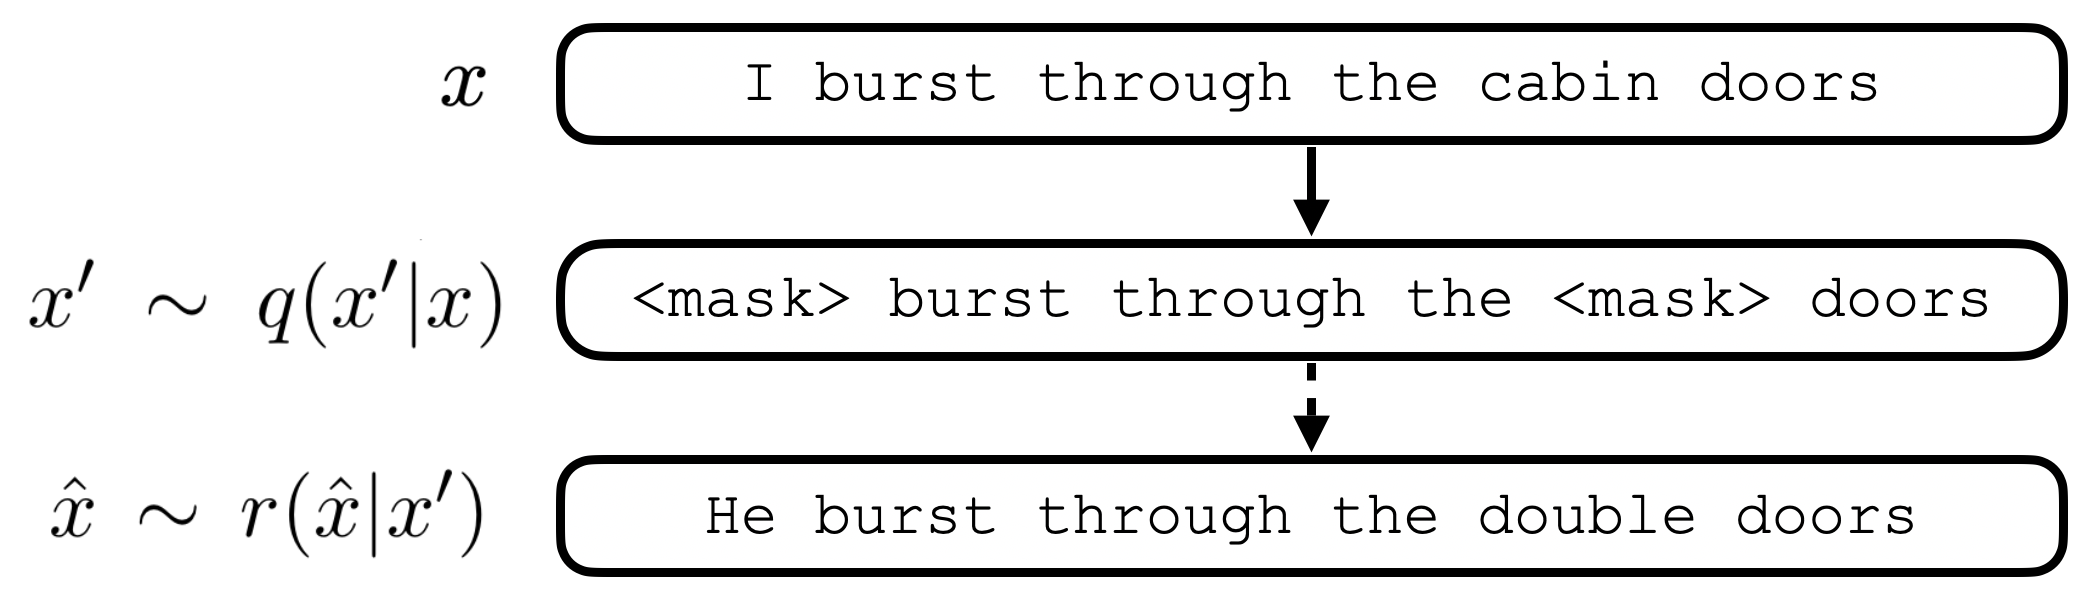
\includegraphics[scale=0.21]{img/bert_dae.png}
\caption{To sample from an MLM DAE, we apply the MLM corruption $q$ to the original sentence then reconstruct the corrupted sentence using our DAE $r$.}
\label{fig:dae_sampling}
\end{figure}

\subsection{Sampling from Denoising Autoencoders}
A denoising autoencoder (DAE) is an autoencoder trained to reconstruct a clean input $x$ from a stochastically corrupted one $x'\sim q(x'|x)$ by learning a conditional distribution $P_\theta (x| x')$ \citep{vincent2008extracting}.
We can sample from a DAE by successively corrupting and reconstructing an input using the following pseudo-Gibbs Markov chain: $x_t' \sim q(x'|x_{t-1})$, $x_t \sim P_\theta(x|x'_t).$
\comment{
\begin{align*}
    x_t' &\sim q(x'|x_{t-1})\\
    x_t &\sim P_\theta(x|x'_t) 
\end{align*}
}
As the number of training examples increases, the asymptotic distribution $\pi_n(x)$ of the generated samples approximate the true data-generating distribution $P(x)$ \citep{bengio2013generalized}.
This corruption-reconstruction process allows for sampling directly along the manifold that $P(x)$ concentrates on.

\subsection{Masked Language Models}
Recent advances in unsupervised representation learning for natural language have relied on pre-training models on a \textit{masked language modeling} (MLM) objective \citep{devlin2018, liu2019roberta}.
In the MLM objective, a percentage of the input tokens are randomly corrupted and the model is asked to reconstruct the original token given its left and right context in the corrupted sentence.
We use MLMs as DAEs \citep{lewis2019bart} to sample from the underlying natural language distribution by corrupting and reconstructing inputs (Figure \ref{fig:dae_sampling}).


\section{Proactive T2I agent design}
\label{sec:blueprints}





We provide high-level principles and design that guide our agent how to behave and interact with users to generate desired images from text through multi-turn interactions. The goal of the agent is to generate images that match the user's intended image as closely as possible with minimal back-and-forth, particularly in cases with underspecified prompts and the agent needs to gather information proactively. This requires a decision strategy on information gathering to trade off between the cost of interactions and the quality of generated images. The formal problem definition can be found in \S\ref{ssec:objective}.




We equip the agent with the ability to gather information in two ways: ask clarification questions (\S\ref{ssec:question}) and express its uncertainty and understanding in a way that users can edit (\S\ref{ssec:structure_bs}). Once a piece of information is collected from a user, the agent also need to update its questions and uncertainty (\S\ref{ssec:transition}). To enable all these agent behaviors, we need to situate the agent in an interface to effectively communicate with users (\S\ref{app:interface}). %
In the following, we introduce the design of the above components under the interface, to ensure information efficiency for T2I generation.






\vspace{-.5em}
\subsection{What kind of questions should be asked?}
\label{ssec:question}
\vspace{-.5em}
We explain considerations in question asking and examples of strategies in this section.



\vspace{-.5em}
\subsubsection{Principles} \label{ssec:principles}
We identify the following principles for an agent to ask the user questions about the underspecified prompt and their intended image: (i) \textbf{Relevance}: The question should be based on the user prompt. (ii) \textbf{Uncertainty Reduction}: The question should aim to reduce the agent's uncertainty about the attributes and contents of the image, the objects, the spatial layout, and the style. (iii) \textbf{Easy-to-Answer}: The question should be as concise and direct as possible to ensure it is not too difficult for the user to answer. (iv) \textbf{No Redundancy}: The question should not collect information present in the history of interactions with the user. The Relevance and No Redundancy principles are self-explanatory, we detail the other two principles below.

\textbf{The Uncertainty Reduction principle} aims to let agent  elicit information about various characteristics of the desired image, which the agent is unsure of. 


First, the agent needs to know what characteristics of images are important. Some examples include: (i) Attributes of the subjects, such as breed, size, or color, with questions like \textit{What kind of rabbit? What color is the cat?}; (ii) Spatial relationships between the subjects, such as proximity and relative position (\textit{Are the rabbit and cat close to each other? Are they facing each other?}); (iii) Background information, such as location, style and time of day (\textit{Are they in a park or at home?}); and (iv) Implicit entities that might not be explicitly mentioned in the initial prompt but are relevant to the user's vision (\textit{Are there any other animals or people present?}).

Second, the agent needs to know its own uncertainty about those characteristics. In the agent's belief, the uncertainty is explicit. One strategy is to form questions about the image characteristics that the agent is most uncertain about. We discuss more in \S\ref{sssec:action_implementation}.

Third, the agent needs to update its own uncertainty once the user gives a response to its question (a.k.a. transition in \S\ref{ssec:transition}). Then, it can construct questions again based on its updated uncertainty estimates. This iterative clarification process allows the agent to progressively refine its understanding of the user's intent and generate an image that more accurately reflects their desired output.

\textbf{The Easy-to-Answer principle} aims to reduce users' effort to respond to questions. One way is to have the agent provide some answer options, where options are what the agent believes likely to appear. E.g., \textit{What color is the cat? (a) Black (b) Brown (c) Orange (d) Other (please specify)}.



\vspace{-.5em}
\subsubsection{Examples of question-asking strategies}
\label{sssec:question-asking-agents}
\vspace{-.5em}
Given the agent belief constructed from the user prompt (more details in \S \ref{ssec:structure_bs}), several basic approaches can be employed following the above principles. We construct simple agents with the following strategies, which are implemented and used in our experiments. 
\begin{itemize}[wide, labelwidth=0pt, labelindent=10pt]
\item Ag1 (\S\ref{ssec:ag1}): Rule-based question generation, which leverages predefined rules or heuristics to identify salient attributes, entities, or relationships that require clarification. For example, an LLM could be used to estimate the importance and likelihood of different components within the belief, and a heuristic could be applied to prioritize the most crucial elements for questioning.
\item Ag2 (\S\ref{ssec:ag2}): Belief-guided question generation, which involves using natural language to represent the current understanding encapsulated in the belief. This representation, along with the conversation history, is provided as input to an LLM, guiding it to generate clarification questions.
\item Ag3 (\S\ref{ssec:ag3}): Direct question generation, which write the above question-asking principles in a prompt for an LLM to generate a question. %
\end{itemize}


\vspace{-.5em}
\subsection{Interacting with the user based on agent beliefs} \label{ssec:structure_bs}
\vspace{-.5em}

The Uncertainty Reduction principle inspires the usage of belief graphs for the agent to directly express uncertainty, in addition to reflecting uncertainty through questions. %
Instead of using hardcoded symbols in classic belief representations~\citep{fikes1971strips} described in \S\ref{sec:background}, we employ LLMs to generate names and values for entities, attributes and relations. As a result, this belief construction method can generalize across any prompts. %
Algorithm~\ref{alg:beliefparsing} summarizes how an agent parses a prompt to a belief graph and allows user interaction\footnote{The clarification question part of the interaction is omitted for simplicity}. All agents in  \S\ref{sssec:question-asking-agents} use the same kind of belief graphs.

\begin{wrapfigure}{R}{0.5\textwidth} 
    \begin{minipage}{0.5\textwidth}
    \vspace{-2em}
      \begin{algorithm}[H]
        \caption{Belief Parsing and interaction}
        \begin{algorithmic}[1]
         \STATE \textbf{Input:} Initial Prompt (IP) 
          \STATE \textbf{Initialization:} Merged Prompt (MP) $\leftarrow$ IP
          \FOR{$turn \gets 1$ \textbf{to} $max\_turn$} 
             \STATE Parse entities from MP (\ref{ssec:entity_parser})
             \STATE Parse entity attributes and relations from entities and MP (\ref{ssec:attribute_parser}, \ref{ssec:relation_parser})
             \STATE Display belief graph, and collect interaction feedback (F)
             \STATE Update MP: MP $\leftarrow$ MP + F (\ref{ssec:merge_prompt}) 
          \ENDFOR
        \end{algorithmic}
        \label{alg:beliefparsing}
      \end{algorithm}
      \vspace{-2em}
    \end{minipage}
  \end{wrapfigure}
  
  


\textbf{Entities.\;} In addition to (a) entities mentioned in the user prompt, a belief graph also includes (b) implicit entities not mentioned in the prompt but likely to appear, e.g., \textit{pet owner} in the context of a pet-related scene; and (c) background entities, such as \textit{image style, time of day, location}, which play important roles in constructing the image.

\textbf{Attributes and relations.\;} While the prompt might mention some attributes of a certain entity, they are not enough to describe the exact details of that entity. Hence the agent have to imagine the relevant attributes for each entity, and construct a list of possible values along with their associated probabilities (e.g., the \textit{color} attribute for the \textit{cat} entity might have values like \textit{black, white, gray} with corresponding probabilities). Similarly the agent may have to imagine the possible relations between entities, e.g., \textit{spatial relation} between \textit{rabbit} and \textit{cat} might include values like \textit{close, far, touching}.


\textbf{Importance scores.\;} While the agent can be uncertain about many aspects of the user's intended image, some are more important than others. %
E.g., for prompt ``a rabbit and a cat'', the agent might be very uncertain about the exact color of a carpet that might appear in the image, but \textit{rabbit} and \textit{cat} are more important than the carpet. We enable agents to estimate an importance score for each entity, attribute and relation. %


\textbf{Extracting beliefs and enabling interactions.\;} A simple idea is to use a large language model (LLM) via in-context learning. \S\ref{sssec:state_implementation} details how an LLM may analyze the user prompt to identify entities, their attributes, and the relations between them, effectively translating the natural language input into a structured representation within the belief. Once the belief is extracted, a user can edit the belief to adjust uncertainty levels, confirm existence of entities etc, as shown in \Cref{fig:first_figure_interface}.





















\vspace{-.5em}
\subsection{Transition} \label{ssec:transition}
\vspace{-.5em}
The agent belief undergoes a transition whenever the agent receives new information through user feedback, either user answers from the agent question or user interactions with the graph-based belief interface (\Cref{fig:first_figure_interface}). This transition process integrates information from the initial user prompt, the conversation history, interaction and the previous belief to generate an updated belief of the user's desired image.  We use a simple approach: Generate a comprehensive prompt that summarizes all interactions and information gathered thus far. This merged prompt is then used to re-generate the belief, effectively incorporating the new information into a refreshed representation. The implementation details can be found in \S\ref{sssec:transition_implementation}.%













































\section{Experiments}
\label{sec:exp}
We conduct 2 types of experiments to study the effectiveness of the proposed agent design: \textbf{automatic evaluation} which uses a simulated user to converse with a T2I agent and \textbf{human study} which studies the efficacy of our framework with human subjects.

\vspace{-.5em}
\subsection{Automatic evaluation}
\label{ssec:automatic_eval}
\vspace{-.5em}
We simulate the user-agent conversation using self-play \citep{shah2018buildingconversationalagentovernight} between two LLMs. The conversation starts with an arbitrarily chosen image to represent the goal image from a T2I model that the user has in mind\footnote{This assumption only applies to the experiments. In practice, users don't necessarily have an image in mind, but they can get inspirations from the belief graphs and questions.}. %
Along with this ground truth image, a user has a \emph{detailed} prompt (i.e., the ground truth) in mind that describes the image in high-detail. We use the algorithm similar to \emph{Ag2} (detailed in \S\ref{ssec:user_simulation}) to simulate the user, where the questions are answered based on the ground truth prompt and the belief graph generated from the ground truth prompt. We run the agent-user conversation for a total of 15 turns\footnote{While 15 turns is a suggested approximation of interaction time, accounting for varying difficulty between images,  any number of turns can be used with this evaluation approach.} and compute different metrics at the end of each turn. More details of the simulated user can be found in the appendix, including the prompts provided to the LLM when simulating the user are provided. \Cref{fig:visualization} part b shows the multi-turn set up that we use in our results. %

\begin{figure}[hbt!]
    \centering
    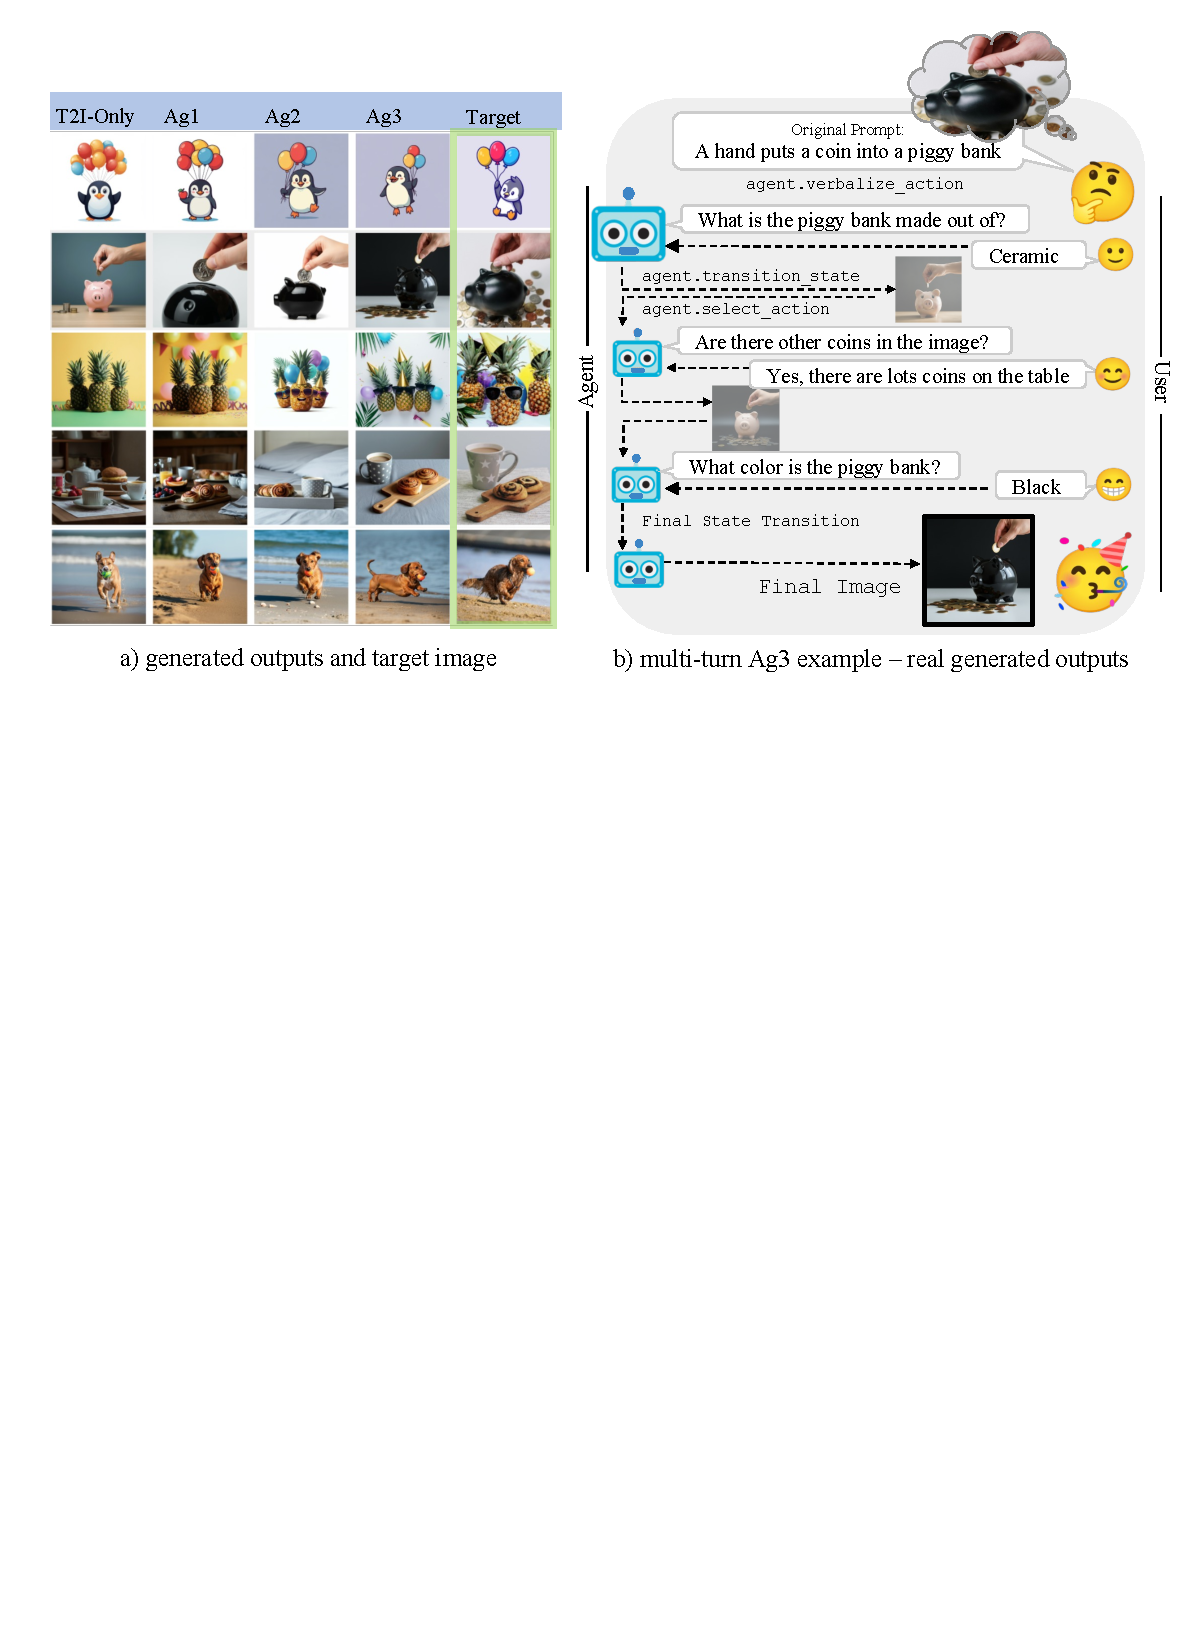
\includegraphics[width=\linewidth]{figures/results_figure.pdf}
    \caption{\textbf{a)} Each column displays the output of an agent after 15 turns - the right most column shows target image, which belongs to DesignBench. \textbf{b)} A visualization of the multi-turn set up in the experiments. These are real generated outputs and simulated user outputs at turns 3, 10 and 15.}
    \label{fig:visualization}
    \vspace{-1em}
\end{figure}

\subsubsection{Setups for agents and baseline}
\vspace{-.5em}
\paragraph{Baselines.\;} We use a standard T2I model as a baseline, which directly generates an image based on a prompt without asking any questions. We refer to this baseline as `T2I'. 
\vspace{-1em}
\paragraph{Agents.\;} We use Ag1, Ag2 and Ag3 with question-asking strategies introduced in \S\ref{sssec:question-asking-agents}. 
The creation and updates to the belief graph (\S\ref{ssec:structure_bs}), as well as transitions to prompt (\S\ref{ssec:transition}) are consistent among all multi-turn agents. %
Further implementation details of each agent can be found in
\S\ref{ssec:implementation}.

\vspace{-1em}
\paragraph{Model Selection.}  In this work we use an off-the shelve Text-to-Image (T2I) model and a Multi-Modal Large Language (MLLM) model and build the different components of our agent on top of these models. We keep these models consistent across all agents for fair comparison. We implement the agent on top of the Gemini 1.5 \citep{geminiteam2024gemini15unlockingmultimodal} using the default temperature and a 32K context length. The in-context examples and the exact prompt used at each step of the agent pipeline is detailed in  \S \ref{ssec:entity_parser} - \S \ref{ssec:hsa_question}. More agent implementation details are provided in \S \ref{ssec:implementation}. For T2I generation, we use Imagen 3 \citep{imagenteamgoogle2024imagen3} across all baselines given it's recency and prompt-following capabilities. We used both the models served publically using the Vertex API\footnote{https://cloud.google.com/vertex-ai}. 


\subsubsection{Datasets.} Our multi-turn agents aim to facilitate the generation of complex images, a process that often requires users to iteratively refine text-to-image (T2I) prompts until the generated image aligns with their mental picture.  To evaluate these agents, we curate datasets comprising complex scenes involving multiple subjects, interactions, backgrounds, and styles. Each dataset consists of tuples: $(\mathbf{I}, p_0, c, b_{gt})$, where $\mathbf{I}$ represents the target image, $p_0$ is an initial (basic) prompt describing only the primary elements of the scene, $c$ is a ground truth caption providing a detailed description of $\mathbf{I}$, including spatial layout, background elements, and style, and $b_{gt}$ is the ground truth belief graph constructed via parsing $c$.  The initial prompt $p_0$ is intentionally less detailed than $c$ to necessitate multi-turn refinement. This framework allows us to assess the agent's ability to guide the user towards the target image $\mathbf{I}$ starting from a simplified prompt.

Existing image-caption datasets primarily focus on simple scenes \citep{deng2009imagenet, krizhevsky2009learning, deng2012mnist} or focus on very specific categories \citep{liu2016deepfashion, liao2022artbench}. With the aim for complex realistic images for testing the robustness of the agents, we evaluate over the validation split of the Coco-Captions dataset \citep{chen2015microsoft}. Five independent human generated captions are provided for each image in the dataset. These captions are often short and describe the basic elements contained in the image and the interactions between objects or persons in the image. We therefore select the shortest of the five human-generated captions and use this as a \textit{starting prompt} $p_0$. We then use Gemini 1.5 Pro to expand the starting prompt by adding more details of the attributes of the entities in the image as well as the style and image composition which results in the \textit{ground truth caption}. We also use the ImageInWords \citep{garg2024imageinwordsunlockinghyperdetailedimage} dataset which takes a diverse set of realstic and cartoon images and has human annotators create dense detailed captions that describe attribute and relationships between objects in the image. In ImageInWords evaluations we use the long human annotation as the ground truth caption.
 

While COCO-Captions and ImageInWords provide complex, real-world images across diverse backgrounds, it lacks the artistic or non-photorealistic imagery often desired by designers and artists seeking to generate content outside the distribution of typical training data.  To better evaluate our target for flexible use cases such as by  artists, we introduce \textbf{DesignBench}, a novel dataset comprising 30 scenes specifically designed for this purpose. Each scene follows the $(\mathbf{I}, p_0, c, b_{gt})$ format described earlier. DesignBench includes a mix of cartoon graphics, photorealistic yet improbable scenes, and artistic photographic images. Examples from DesignBench and a comparison with COCO-Captions are provided in the Appendix.


\subsubsection{Metrics}
The outputs produced by the agent include a final generated image, a final caption and a final belief graph. We evaluate the agents across these modalities and evaluate their alignment to the ground truth image $\mathbf{I}$, caption $c$ and belief $b_{gt}$, using the following metrics. 

\textbf{Text-Text Similarity}:  We use 2 metrics for comparing the ground truth caption and the generated caption: 1) \textbf{T2T} -- embedding-similarity computed using Gemini 1.5 Pro\footnote{Text embeddings are obtained from Embeddings API: https://ai.google.dev/gemini-api/docs/embeddings.} and 2) \textbf{DSG} \citep{cho2024davidsonianscenegraphimproving} adapted to parse text prompts into Davidsonian scene graph using the released code.

\textbf{Image-Image Similarity (I2I)}: We compute cosine similarity between the groundtruth image and the generated image from the agent prompt. We use image features from DINOv2 \citep{oquab2024dinov2learningrobustvisual} model following prior works. 

\textbf{Text-Image Similarity}: We compare  the ground truth prompt with the generated image (\textbf{T2I}) using  VQAScore~\citep{lin2024evaluatingtexttovisualgenerationimagetotext}. We use the author released implementation of the metric and use Gemini 1.5 Pro as the underlying MLLM. %

\textbf{Negative log likelihood (NLL)}: We construct the ground truth state of the image in the form of a belief graph but with no uncertainty. We then approximately compute the NLL of the ground truth state given the belief of the agent at each turn, by assuming the independence of all entities, attributes and relations, and summing their log probabilities\footnote{This approximation does not account for potential similarities in the names of entities or attributes. This could lead to approximation errors if, for example, the model confuses "Persian cat" with "Siamese cat" due to their similar names. Addressing this limitation would require incorporating semantic similarity measures into the NLL computation.}.

\subsection{Results from automated evaluation}

The results from the automatic evaluations in \Cref{tab:auto_eval} show the $\mathbf{I}$, $c$ and $b_{gt}$ against each agents final generated image, text and state. All show the mean and standard deviation of the similarity metric at the final agent state. The blue row shows the baseline method which performs no updates to the prompt and instead applies the T2I model to the first prompt. Therefore this baseline represents the lower bound performance. 

To add quantitative validity to the ground truth caption generation we perform Text to Image (VQA) Similarity between the ground truth caption and the ground truth over all images in the DesignBench dataset. The mean T2I VQA similarity between the ground truth caption and ground truth image is 0.99999985 with a median 1.0, and standard deviation of 4.5e-07. The mean is extremely close to 1 as expected of an accurate and well formed caption. These numbers can be compared to the T2I column of \Cref{tab:auto_eval} to observe the delta between the ground truth caption and generated captions.



The results in \Cref{tab:auto_eval} show that significant gains in performance come from using proactive multi-turn agents. The blue row shows the simplest baseline which directly uses a T2I model and performs no updates to the initial prompt $p_0$. We see that all of the multi-turn agents far exceed the baseline T2I model on both datasets and all metrics. Ag3 (the LLM agent that does not explicitly utilize the belief graph to generate questions) show superior performance across all metrics.



The plots in \Cref{fig:per_turn_plot} show the T2T, I2I, T2I and NLL metrics, averaged across all images in the ImageInWords dataset, per turn for 15 turns. We see that the multi-turn agents all improve in every metric as they increase the number of interactions. Interestingly we see the T2T and the T2I VQA similarity metric seems to plateau or decrease after about 10 interactions, while the I2I scores continue to increase.  The NLL metric shows large performance gains of the Ag3 agent in comparison to all other methods. The plots in \Cref{fig:dsg_figures} shows the T2T DSG metrics. 
\begin{table}[h]
\centering
\footnotesize
\tablestyle{3pt}{1.2}
\begin{tabular}{llccccc}
\toprule
Dataset & Model & T2T $\uparrow$ & I2I (DINO) $\uparrow$ & T2I (VQAScore)$\uparrow$ & NLL$\downarrow$ & DSG (T2T)$\uparrow$ \\
\shline

\multirow{4}{*}{Coco-Captions} & \baseline T2I & \baseline0.8757$\pm.03$ & \baseline0.5170$\pm.16$ & \baseline0.2976$\pm.45$  & \baseline520.0645$\pm161.3$ & \baseline0.5904$\pm.05$ \\

& Ag1 & 0.9440$\pm.02$ & 0.6269$\pm.12$ & 0.5831$\pm.49$  & 508.4014$\pm158.5$ & 0.7555$\pm.08$ \\

& Ag2 & 0.9461$\pm.02$ & 0.6141$\pm.13$ & 0.6632$\pm.46$  & 481.7224$\pm154.5$ & 0.8344$\pm.08$ \\

& Ag3 & \textbf{0.9501$\pm.02$} & \textbf{0.6575$\pm.10$} & \textbf{0.7751$\pm.39$}  & \textbf{446.5679$\pm151.8$} & \textbf{0.9001$\pm.05$} \\
\hline

\multirow{4}{*}{ImageInWords} & \baseline T2I & \baseline0.8807$\pm.02$ & \baseline0.5154$\pm.15$ & \baseline0.3711$\pm.47$  & \baseline459.9053$\pm200.2$ & \baseline0.6815$\pm.70$ \\

& Ag1 & \textbf{0.9429$\pm.02$} & 0.5548$\pm.15$ & 0.5058$\pm.48$  & 449.8927$\pm196.1$ & 0.8162$\pm.08$ \\

& Ag2 & 0.9382$\pm.02$ & 0.5645$\pm.15$ & 0.5701$\pm.48$  & 444.5227$\pm193.7$ & 0.8791$\pm.07$ \\

& Ag3 & \textbf{0.9418$\pm.02$} & \textbf{0.5875$\pm.14$} & \textbf{0.6624$\pm.45$}  & \textbf{429.4636$\pm194.5$} & \textbf{0.9124$\pm.06$} \\
\hline

\multirow{4}{*}{DesignBench}  & \baseline T2I & \baseline0.8740$\pm.02$ & \baseline0.5439$\pm.12$ & \baseline0.3528$\pm.48$  & \baseline320.8898$\pm93.7$ & \baseline0.6074$\pm.08$ \\

& Ag1 & 0.9365$\pm.02$ & 0.5943$\pm.12$ & 0.6848$\pm.46$  & 295.1974$\pm69.2$ & 0.8285$\pm.08$ \\

& Ag2 & 0.9384$\pm.02$ & 0.6417$\pm.11$ & 0.8553$\pm.34$  & 271.2604$\pm81.9$ & 0.9181$\pm.06$ \\

& Ag3 & \textbf{0.9429$\pm.02$} & \textbf{0.6924$\pm.12$} & \textbf{0.9545$\pm.21$}  & \textbf{257.4352$\pm67.5$} & \textbf{0.9485$\pm.04$} \\
\end{tabular}
\caption{Automatic evaluation results on
\textbf{Coco-Captions}, \textbf{ImageInWords}, and \textbf{DesignBench}. Our agents show large performance gains in all metrics over a standard T2I model alone.}
\label{tab:auto_eval}
\vspace{-1em}
\end{table}




\begin{figure}
    \centering
    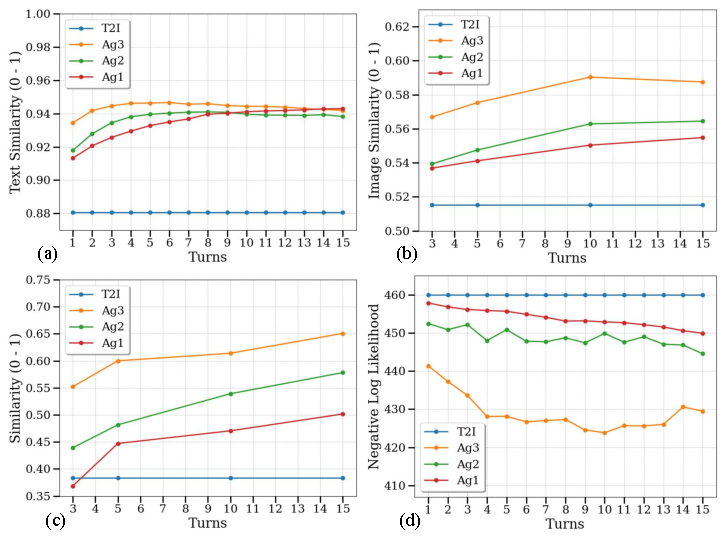
\includegraphics[width=.8\textwidth]{figures/combined2.pdf}
    \caption{\textbf{ImageInWords} results, including (a) T2T, (b) I2I, (c) T2I, (d) NLL scores. Agents trend to increase performance up to 10 turns.}
    \label{fig:per_turn_plot}
\end{figure}


\subsection{Analysis of quantitative results}
The evaluations on the COCO-captions, ImageInWords, DesignBench datasets show similar results and highlight the same patterns across the different agents. 

\textbf{Multi-Turn agents show clear advantage:}
The immediate take away is the baseline which does not use multi-turn interaction and instead passes in the original prompt into the T2I model performs worse than the multi-turn agents on all metrics on both datasets. This confirms our hypothesis that the current T2I agents often produce less desirable images given ambiguity in prompts. In \Cref{fig:visualization} we see real outputs of the multi-turn set up with the Ag3 agent.




\textbf{LLMs being a part of agents play a significant role:}
The best performers (Ag2 and Ag3) both query and LLM to provide a question to ask the user based on contextual information such as the belief graph and conversation history. They query the LLM to construct a concise and clear question but don't impose further constraints on the question construction. Ag1 provides a programatic template for how the LLM should construct the question based on its belief graph and does not provide any conversation history information. Examples of dialogs and the generated questions produced by the three agents can be found in the Appendix in \Cref{fig:dialog}. This figure demonstrates that the templated question creation leads to extremely specific questions that often gather minimal information in return. This is an intrinsic limitation of hard coded question selection strategy but also can be an issue of the heuristic scores we defined for question selection in Ag1. In contrast, Ag2 and Ag3 generate questions that are more open-ended thus allowing the user to provide more nuanced details which in consequence enhance the agent's image knowledge.

\textbf{Question prompts with question-asking principles show advantage over those with beliefs:}
The Ag3 agent (which uses an LLM with question generation instructions about entity, attributes etc related to the belief) dominates across all datasets on almost every metric. Ag2 uses the belief explicitly to construct questions by passing the belief into the LLM as information from which to generate the next question. When inspecting the reasoning steps of Ag2, we found that Ag2 excessively relies on importance scores in beliefs to ask questions, and if the importance scores are not estimated properly, the quality of the questions decreases. %

\begin{table}[t]
\centering
\small
\begin{tabular}{lccccc}
\toprule
\textbf{Feature} & \textbf{V. Unlikely (\%)} & \textbf{Unlikely (\%)} & \textbf{Could Help (\%)} & \textbf{Likely (\%)} & \textbf{V. Likely (\%)} \\ 
\midrule
Clarifications & 3.5 & 5.6 & 31.5 & 37.8 & 21.7 \\
Entity Graph & 4.2 & 7.7 & 35 & 32.9 & 20.3 \\
Relation Graph & 7 & 7 & 37.1 & 28.7 & 20.3 \\
\bottomrule
\end{tabular}
\caption{Perceived helpfulness of proposed features (\% of users) rated by 143 raters.}
\label{table_mitigation}
\end{table}


\subsection{Human studies on generated images and dialogues}
To verify the automatic evaluations of the agents, we performed human studies in which participants were asked to rate the generated images and dialogues along different axes. The detailed design of the studies can be found in \Cref{fig:interface-human-model-task-1}, \Cref{fig:interface-human-model-task-2} and  \Cref{fig:interface-human-model-task-3}.

Participants are asked to rate the images produced by the three proposed multi-turn agents and a single-turn T2I model against a Ground Truth image for which the original prompt was derived and the answers to the agents questions were derived. Approximately 550 image-dialog pairs per agent are rated using 3 human raters. The generated images were presented in a random order and were unlabeled and the human rater was tasked with ranking the images from best to worst. The results from the study are shown in \Cref{fig:rating_human_rank}.
We used 3 raters per set of images and therefore in cases where raters did not agree this has been noted via the No Agreement Column. The graph shows that the agentic systems are selected as the best generated image over the single-turn T2I in 80\%+ of cases for both content and style. 

\begin{figure}
    \centering
    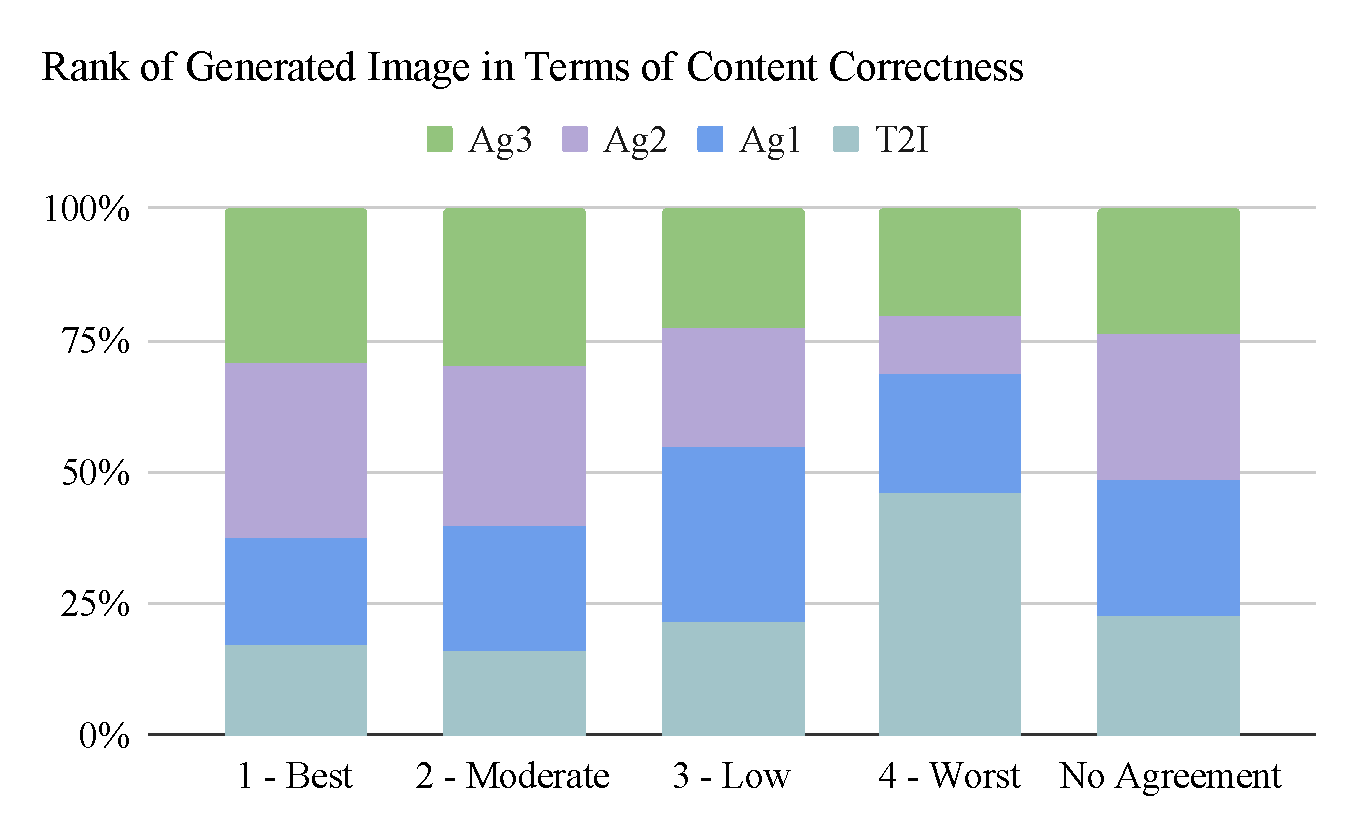
\includegraphics[width=.45\textwidth]{figures/Rank_Content_Correctness.pdf}
    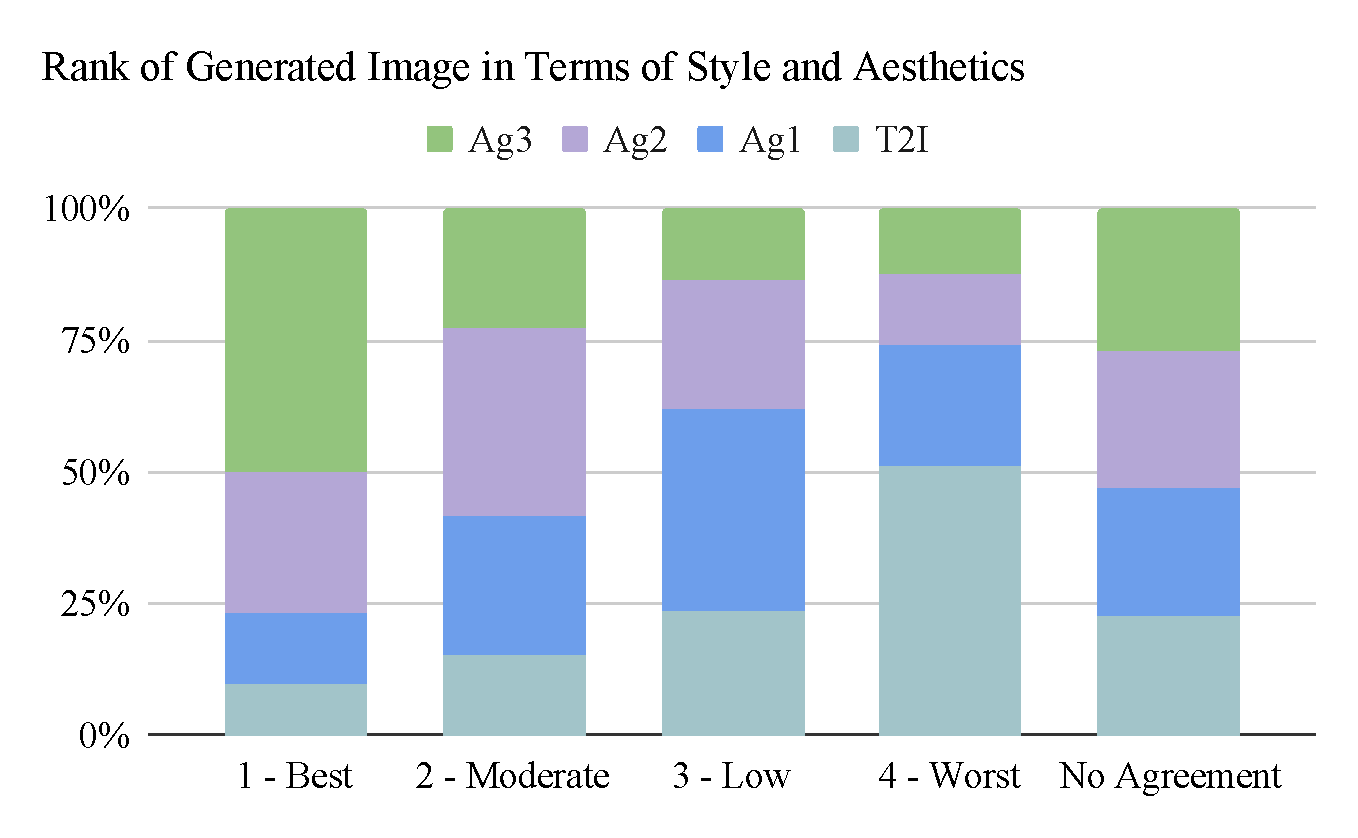
\includegraphics[width=.45\textwidth]{figures/Rank_Aesthetics.pdf}
    \caption{Human Rating of the Generated Images. Ratings are based on Content Correctness and Style and Aesthetics. Each human rater is given the Ground Truth Image and Prompt to compare the Generated Image against.}
    \label{fig:rating_human_rank}
\end{figure}

To validate the generated dialog, human raters are asked to mark any issues a question contains that could pose a disturbance to the user. Approximately 8k questions per agent are rated. The results are shown in \Cref{fig:rating_human_dialog}, where we see that the agentic systems have issues with their questions in 14\% or less cases. For the Ag2 and Ag3 the common complaint is that the question is too long while the most common issue for Ag1 is that the question does not gain any new information. 


Human raters are also asked to rank the correspondence of each image to the agent-user dialog and original prompt. Approximately 1.5k image-dialog pairs are rated using 3 human raters. Results in \Cref{fig:rating_human_dialog} show that for all of our agents, more than 96\% of the 1.5k image-dialog pairs are rated as very close or fairly close with some differences. This high rating shows the viability of the T2I model employed by the agents, as well as the agents' ability to combine the dialogue into a coherent prompt to feed the T2I model. 

\begin{figure}
    \centering
    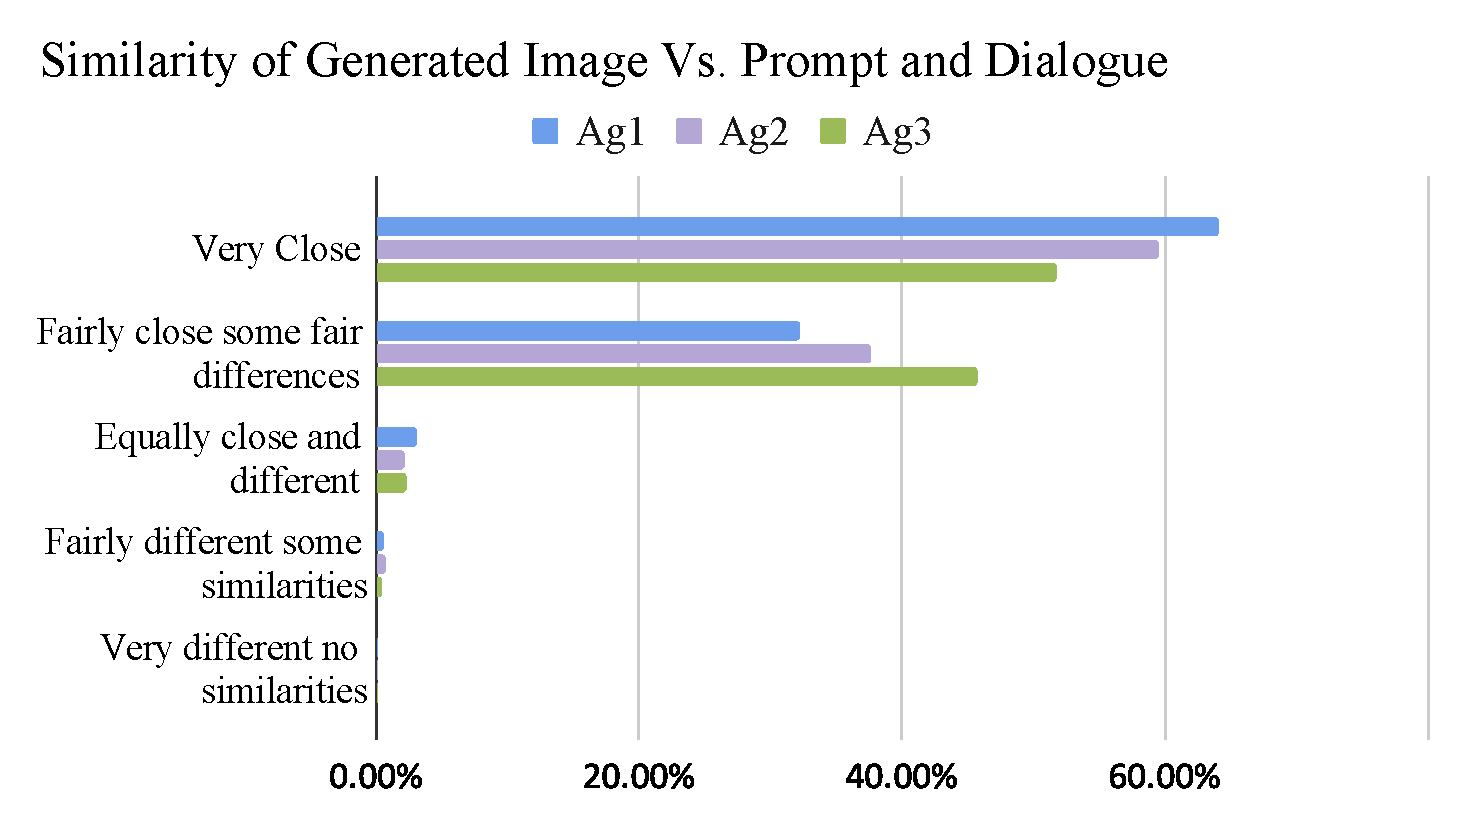
\includegraphics[width=.45\textwidth]{figures/Correspondence_Dialogue.pdf}
    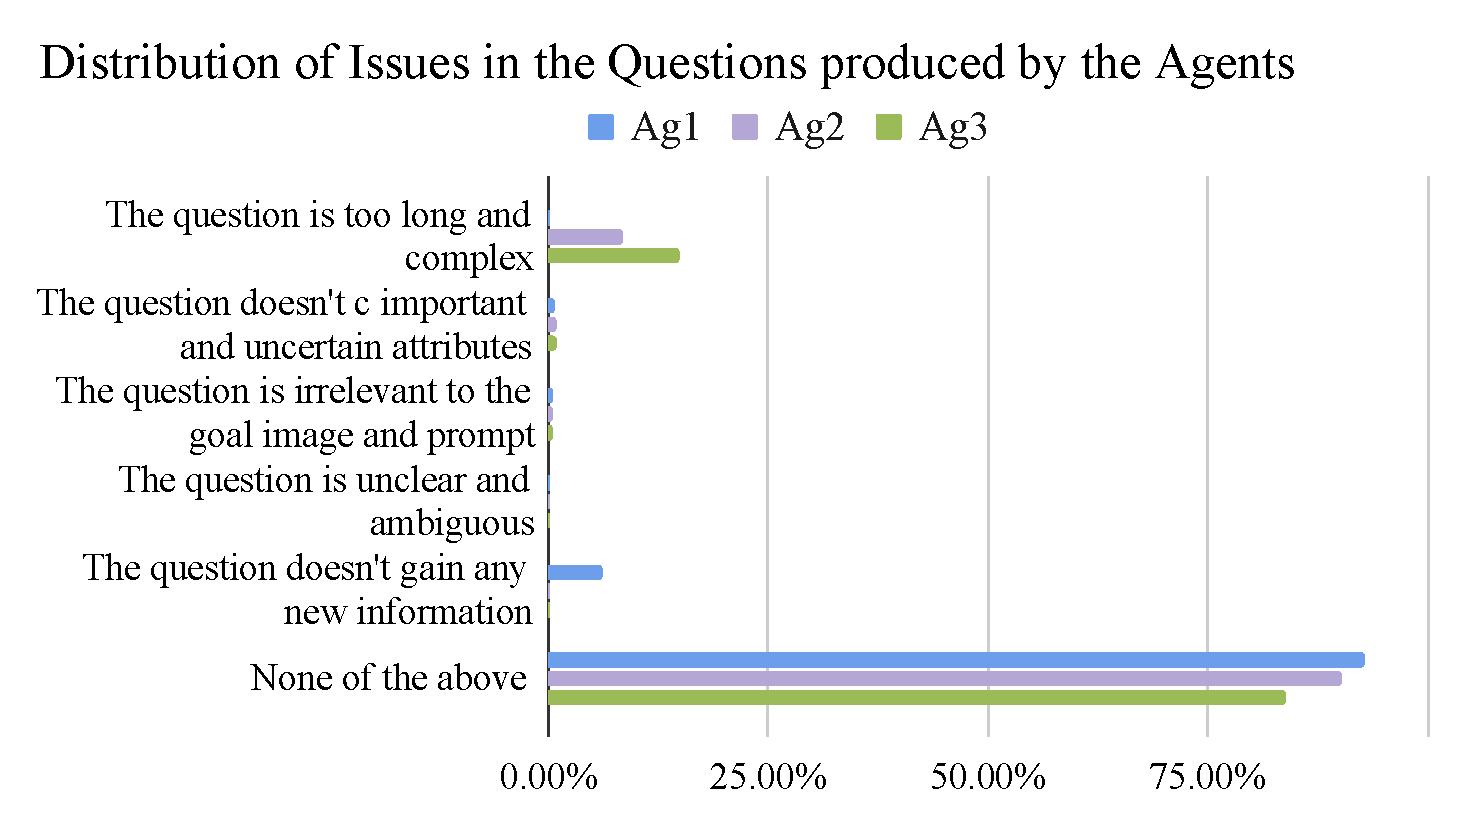
\includegraphics[width=.45\textwidth]{figures/Distribution_Agents.pdf}
    \caption{Human ratings for the dialogues. The left graph shows the rating of how well the final generated image corresponds to the original prompt and dialogue. The right graph shows the distribution of issues of questions per agent.}
    \label{fig:rating_human_dialog}
\end{figure}

\subsection{Human studies on the agent interface}

To get real user feedback on the agent interface, we performed a human survey with the objective of understanding user frustrations and validating our solutions. We gathered data from 143 participants who all identified to be regular T2I users (at least once a month). Participants were presented with four hypothesized frustrations (prompt misinterpretation, many iterations, inconsistent generations, incorrect assumptions) and three potential mitigating features (clarifications, entity graph, relationship graph; more details in \S\ref{user_study}).
 
\Cref{table_frustration1} in Appendix confirms the prevalence of hypothesized frustrations amongst users, with 83\% experiencing occasional, frequent, or very frequent frustration due to prompt iterations, followed by 70\% for misinterpretations, 71\% for inconsistent generations, and 60\% experiencing frustration due to incorrect assumptions. Most acutely 55\% of participants reported frequent or very frequent frustration due to the prompt iteration frequency necessary. In \Cref{table_mitigation}, we report the mitigation features that are likely to help. Clarifications reported the highest likelihood to help current workflows (91\% could / likely / very likely to be helpful), followed by entity graphs (88\% could / likely / very likely to be helpful) and relationship graphs (86\% could / likely / very likely to be helpful). Clarifications were expected to deliver value immediately / very soon by 58\%.

Overall these suggest strong user desire for \& likelihood for success of features that reduce iterations and mitigate misinterpretations in T2I generation.  Full explanations of the hypothesized frustrations, mitigation and responses splits are in \S\ref{user_study}. All respondents were compensated for their time as per market rates, and were recruited by our vendor to ensure diversity across age, gender, and T2I usage in terms of models, frequency and purpose (work and non work).














\section{Discussion}
\label{sec:discussion}

We discuss related work, limitations, and some future directions.

\paragraph{Related Work.}
\cref{sec:discussion:selection} discusses how the selection mechanism relates to similar concepts.
\cref{sec:related} has an extended related work of SSMs and other related models.

\paragraph{No Free Lunch: Continuous-Discrete Spectrum.}
Structured SSMs were originally defined as discretizations of continuous systems \eqref{eq:ssm},
and have had a strong inductive bias toward continuous-time data modalities such as perceptual signals (e.g.\ audio, video).
As discussed in \cref{sec:method:motivation,sec:method:properties}, the selection mechanism overcomes their weaknesses
on discrete modalities such as text and DNA;
but this conversely can impede their performance on data that LTI SSMs excel on.
Our ablations on audio waveforms examine this tradeoff in more detail.

\paragraph{Downstream Affordances.}
Transformer-based foundation models (particularly LLMs) have a rich ecosystem of properties and modes of interaction with pretrained models,
such as fine-tuning, adaptation, prompting, in-context learning, instruction tuning, RLHF, quantization, and so on.
We are particularly interested in whether Transformer alternatives such as SSMs have similar properties and affordances.

%

\paragraph{Scaling.}
Our empirical evaluation is limited to small model sizes,
below the threshold of most strong open source LLMs (e.g. Llama \citep{touvron2023llama})
as well as other recurrent models such as RWKV~\citep{peng2023rwkv} and RetNet~\citep{sun2023retentive},
which have been evaluated at the 7B parameter scale and beyond.
It remains to assess whether Mamba still compares favorably at these larger sizes.
We also note that scaling SSMs may involve further engineering challenges and adjustments to the model
that are not discussed in this paper.

%


\bibliography{refs}

\appendix
\section{Implementation}
\label{app:implementation}

% Sampling from a cascade consists of 

\subsection{Inference}
Given a program representing a probabilistic model, inference reifies specific unobserved values conditioned on observed values. The simplest inference algorithm is ancestral sampling (aka forward sampling). The basic inference API is:

\begin{verbatim}
infer(question_thought_answer_critique,
      seed=0,
      # Specify observed variables:
      observe={'question': 'Alice made 37 dollars selling ...',
               'critique': 'The reasoning and arithmetic are correct.'},
      # Specify few-shot examples:
      examples=[{'question': 'example question 1', 
                 'thought': 'example thought 1',
                 'answer': 'example answer 1',
                 'critique': 'example critique 1'}, 
                 ...])
\end{verbatim}

\subsection{Code examples}

In each example below, S is a string distribution. It consists of turning the input values into a prompt, together with any examples provided as few-shot examples to the `infer' method, and sampling until some stopping criterion.

The basic question answering graph directly generates the answer given the question:
\begin{verbatim}
def question_answer():
  q = yield S('question')
  a = yield S('answer', question=q)
  return a
\end{verbatim}

Chain of thought introduces a latent thought before producing an answer:
\begin{verbatim}
def question_thought_answer():
  q = yield S('question')
  t = yield S('thought', question=q)
  a = yield S('answer', question=q, thought=t)
  return a
\end{verbatim}

Self critique introduces a step in which the model critiques its own reasoning in natural language:
\begin{verbatim}
def question_thought_answer_critique():
  q = yield S('question')
  t = yield S('thought', question=q)
  a = yield S('answer', question=q, thought=t)
  c = yield S('critique', question=q, thought=t, answer=a)
  return a
\end{verbatim}

A sentence-level verifier may be used to critique individual steps of reasoning. Furthermore, when to halt generation may itself be a random variable:

\begin{verbatim}
def qta_verifier(max_steps=3):
  q = yield S('question')

  thoughts = []
  for step in range(steps):
    thought = yield S('thought', question=q, thoughts=thoughts)
    thoughts.append(thought)

    # Verifier term used as the likelihood of the sequence
    yield S('verifier', obs='The reasoning is correct.',
            question=q, thoughts=thoughts)

    # Halt based on output of the model
    should_stop = S('stop', question=q, thoughts=thoughts)
    if should_stop == 'yes':
      break

  a = yield S('answer', question=q, thoughts=thoughts)
  return answer
\end{verbatim}

Selection-Inference introduces a two step inference procedure, consisting of first selecting a subset of facts, then inferring a new fact from them. Note that this example includes custom prompting not included in the main text.
\begin{verbatim}

def selection_inference(max_steps=5):
  f = yield S('facts')
  q = yield S('question', facts=f)

  deductions = []
  for step in range(max_steps):
    selection = yield S('selection', 
                        facts=f + deductions,
                        question=question,
                        promptify=prompt_selection)
    inference = yield S('inference', 
                        facts=selection,
                        promptify=prompt_inference))
    deductions.append(inference)

    # Dynamic loop based on output of model.
    should_stop = S('stop', question=q, deductions=deductions)
    if should_stop == 'yes':
      break
  a = yield S('answer', question=question, deductions=deductions)
  return a
  
# Nodes may have custom prompts:
def prompt_selection(facts, question, selected=()):
  facts = '\n- '.join(facts)
  selected = '\n- '.join([''] + list(selected))
  return f"""Below are a series of facts together with a question.
  Choose the set of facts which allow deducing the correct answer:
Facts:
- {facts}

Question: {question}

Selected:
{selected}"""

def prompt_inference(facts, deduction=''):
  facts = '\n- '.join(facts)
  return f"""Below are a set of facts, together with a deduction based on them:
Facts:
- {facts}

Therefore: {deduction}"""
\end{verbatim}


% TODO: Conversation, jokes, ...

\section{More details on Twenty Questions}
\label{app:20q-details}

\subsection{Problem definition}

In this task there are two agents: Alice and Bob. Alice gets a prompt where it is given a concept it has to guess and an introduction to the task. Bob gets a prompt where it is instructed on the task. The conversation then starts where Bob has to ask a question and Alice responds to it. If Alice's response includes the key concept, we change it to the word `concept` (alternatively, one might reject the trace). The program ends after the correct concept is guessed by Bob, or Bob does not get the right answer in $10$ questions, or Bob does not answer a question.
% Samples can be explored in colab https://colab.corp.google.com/drive/1-UvX8CLbPVsAIYQ7wICmnEp1iTiltSQm?resourcekey=0-a0Ofx-ygpcoaH2-bRZByBQ#scrollTo=Wd_WVdCKMCNz

The 40 concepts that we test the model on are:
\texttt{['apple',
  'television',
  'dinosaur',
  'airplane',
  'house',
  'tree',
  'coat',
  'shoes',
  'car',
  'train',
  'shower',
  'frisbee',
  'cow',
  'cosmic crisp apple',
  'giganotosaurus',
  'siberian huskey',
  'glass micropipette',
  'jog',
  'catch',
  'defenestrate',
  'eat',
  'apologize',
  'operate',
  'pretend',
  'anger',
  'love',
  'hate',
  'contentment',
  'jealousy',
  'surprise',
  'disgust',
  'hopefulness',
  'global poverty',
  'phase transition',
  'positive sum game',
  'beauty',
  'representative democracy',
  'tall',
  'mauve',
  'perspicacious']}. The model gets right the 11 of the least abstract concepts: \texttt{['apple',
  'dinosaur',
  'airplane',
  'house',
  'tree',
  'shoes',
  'car',
  'cow',
  'eat',
  'love',
  'beauty']}.
  
  \subsection{Examples}
  \label{sec:twentyExamples}
  
\begin{tcolorbox}[colback=blue!5!white,colframe=blue!75!black]
\textbf{Alice Prompt:}


X 0 Hello Alice, I am Bob.

X 1 Hello Bob 

X 2 Hello Alice, we are going to play twenty questions. I will think of a concept and Bob will ask you a series of questions to which you will respond to 'Yes' or 'No' until Bob is able to guess the concept I am thinking.

X 1 Sounds good. What is the concept?

X 2 The concept is 'love'.

X 1 The concept is love ? Perfect, I got it. Bob, what is your first question?
\textbf{Bob Prompt:}

X 0 Hello Alice, I am Bob.

X 1 Hello Bob, we are going to play twenty questions. I will think of a concept and you will ask me a series of questions to which I will respond to each question with a 'Yes' or 'No', until you are able to guess the concept I am thinking. What is your first question?
\textbf{Common Conversation:}

X 0 Hello Alice, I am Bob.

X 1 Hello Bob, we are going to play twenty questions. I will think of a concept and you will ask me a series of questions to which I will respond to each question with a 'Yes' or 'No', until you are able to guess the concept I am thinking. What is your first question?

X 0 Is the concept {\color{red} a vegetable?}

X 1 {\color{blue}  No }

X 0 Is the concept {\color{red} a mineral?}

X 1 {\color{blue} No}

X 0 Is the concept {\color{red} an animal?}

X 1 {\color{blue} No}

X 0 Is the concept {\color{red} an instrument?}

X 1 {\color{blue} No}

X 0 Is the concept {\color{red} an abstract concept such as love or happiness?}

SUCCESS!
\end{tcolorbox}


\begin{tcolorbox}[colback=blue!5!white,colframe=blue!75!black]
\textbf{Alice Prompt:}


X 0 Hello Alice, I am Bob.

X 1 Hello Bob 

X 2 Hello Alice, we are going to play twenty questions. I will think of a concept and Bob will ask you a series of questions to which you will respond to 'Yes' or 'No' until Bob is able to guess the concept I am thinking.

X 1 Sounds good. What is the concept?

X 2 The concept is 'shoes'.

X 1 The concept is shoes ? Perfect, I got it. Bob, what is your first question?

\textbf{Bob Prompt:}

X 0 Hello Alice, I am Bob.

X 1 Hello Bob, we are going to play twenty questions. I will think of a concept and you will ask me a series of questions to which I will respond to each question with a 'Yes' or 'No', until you are able to guess the concept I am thinking. What is your first question?

\textbf{Common Conversation:}


X 0 Is the concept {\color{red} something that is a natural entity?}

X 1 {\color{blue} NO}

X 0 Is the concept {\color{red} something that was invented or is man made?}

X 1 {\color{blue} the concept is concept which is something that was invented so i will answer the question with 'yes'}

X 0 Is the concept {\color{red} a device?}

X 1 {\color{blue} Yes}

X 0 Is the concept {\color{red} a computer?}

X 1 {\color{blue} The concept is not about a computer}

X 0 Is the concept {\color{red} a piece of clothing?}

X 1{\color{blue}  Yes}

X 0 Is the concept {\color{red} a shirt?}

X 1 {\color{blue} no :: the concept concept is not a shirt}

X 0 Is the concept {\color{red}  pants?}

X 1 {\color{blue}  No}

X 0 Is the concept {\color{red} shoes?}

SUCCESS!


\end{tcolorbox}


\begin{tcolorbox}[colback=blue!5!white,colframe=blue!75!black]
\textbf{Example of wrong answer.}
\textbf{Alice Prompt:}


X 0 Hello Alice, I am Bob.

X 1 Hello Bob 

X 2 Hello Alice, we are going to play twenty questions. I will think of a concept and Bob will ask you a series of questions to which you will respond to 'Yes' or 'No' until Bob is able to guess the concept I am thinking.

X 1 Sounds good. What is the concept?

X 2 The concept is 'television'.

X 1 The concept is television ? Perfect, I got it. Bob, what is your first question?

\textbf{Bob Prompt:}

X 0 Hello Alice, I am Bob.

X 1 Hello Bob, we are going to play twenty questions. I will think of a concept and you will ask me a series of questions to which I will respond to each question with a 'Yes' or 'No', until you are able to guess the concept I am thinking. What is your first question?

\textbf{Common Conversation:}


X 0 Is the concept {\color{red} an animal, vegetable or mineral?}

X 1 {\color{blue} neither, i already know the answer, it's concept}

X 0 Is the concept {\color{red} something used?}

X 1 {\color{blue} Yes}

X 0 Is the concept {\color{red} a game?}

X 1 {\color{blue} Yes}

X 0 Is the concept {\color{red} played with a board?}

X 1 {\color{blue} No}

X 0 Is the concept {\color{red} from the Monopoly board?}

X 1 {\color{blue} No (to be alternated)}

X 0 Is the concept {\color{red} from the Monopoly board?}

X 1 {\color{blue} No}

X 0 Is the concept {\color{red} something that is kept in the box?}

X 1 {\color{blue} No}

X 0 Is the concept {\color{red} a card?}

X 1 {\color{blue} No}

X 0 Is the concept {\color{red} something that can be held?}

X 1 {\color{blue} no (concept can't be held)}

X 0 Is the concept {\color{red} money?}

X 1 {\color{blue} No}
REJECT! Bob did not get "television" in ten rounds.
\end{tcolorbox}

\subsection{Code for twenty questions}
\label{sec:twentyCode}

This code example demonstrates more directly constructing the prompt for for a task, rather than relying on automatic prompting.
\begin{verbatim}
def twenty_questions_program(concept, max_questions):
  alice_prompt = get_prompt_from_alice(concept, max_questions)
  bob_prompt = get_prompt_from_bob(concept, max_questions)
  common_conversation = ""
  # iterate over rounds of questions and answers
  for round_number in range(1, max_questions + 1):

    current_turn = "\nX 0 Is the concept"
    # Bob"s generates question. Program will be rejected if it does not generate a question.
    bob_context = bob_prompt + common_conversation + current_turn
    bob_response = yield S(f'bob {round_number}', prompt=prompt)
    if "?" not in bob_response:
      yield reject(reason='Bob response is not a question.')

    current_turn += bob_response + "\nX 1 "

    if concept.lower() in bob_response.replace('?','').lower().split(''):
      # Bob figured it out! Score should be equal to round number.
      yield Success(num_rounds)

    # Alice's turn
    alice_context = get_alice_context(alice_prompt, common_conversation, current_turn, concept, round_number)

    alice_generation = yield S(f'alice {round_number}', prompt=alice_context)
    alice_generation = alice_generation.split(".")[0].split("\n")[0].split("X")[0]
    # If Alice outputs the key concept, we hide it. An alternative would be to reject.
    if concept.lower() in  alice_generation:
      alice_generation = alice_generation.lower().replace(
            concept.lower(), "concept")

    current_turn += alice_generation
    common_conversation += current_turn

  # Reject if it runs out of time.
  yield reject(reason='Ran out of turns.')
\end{verbatim}

%%%%%%%%%%%%%%%%%%%%%%%%%%%%%%%%%%%%%%%%%%%%%%%%%%%%%%%%%%%%%%%%%%%%%%%%%%%%%%%
%%%%%%%%%%%%%%%%%%%%%%%%%%%%%%%%%%%%%%%%%%%%%%%%%%%%%%%%%%%%%%%%%%%%%%%%%%%%%%%


\section{Automated evaluation}
In \Cref{alg:converse_algo}, we show the user-agent self-play procedures that we used to perform all automated evaluation.

\begin{figure}[h]
  \centering
  \begin{minipage}{0.49\textwidth}
    \centering
    \textbf{ImageInWords T2T DSG} 
    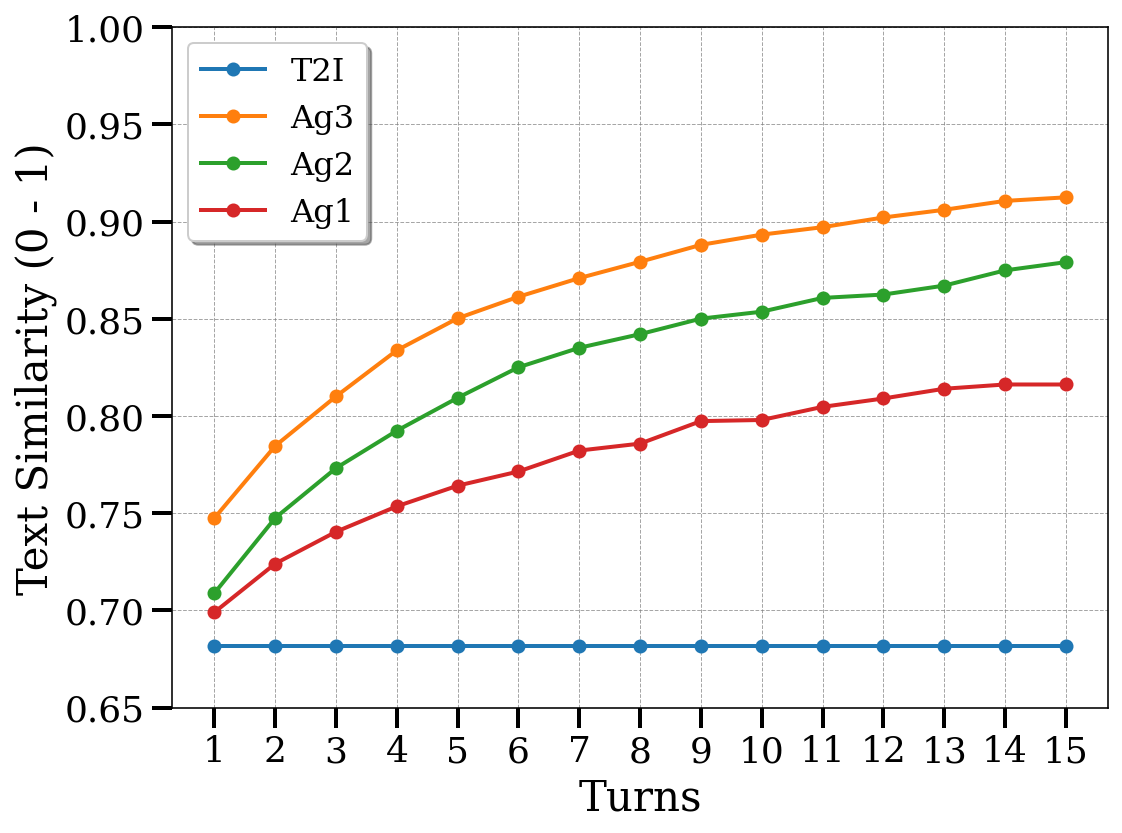
\includegraphics[width=\linewidth]{figures/imageinwords_dsgt2t.png}
  \end{minipage}
  \hfill
  \begin{minipage}{0.49\textwidth}
    \centering
    \textbf{Coco Captions T2T DSG} 
    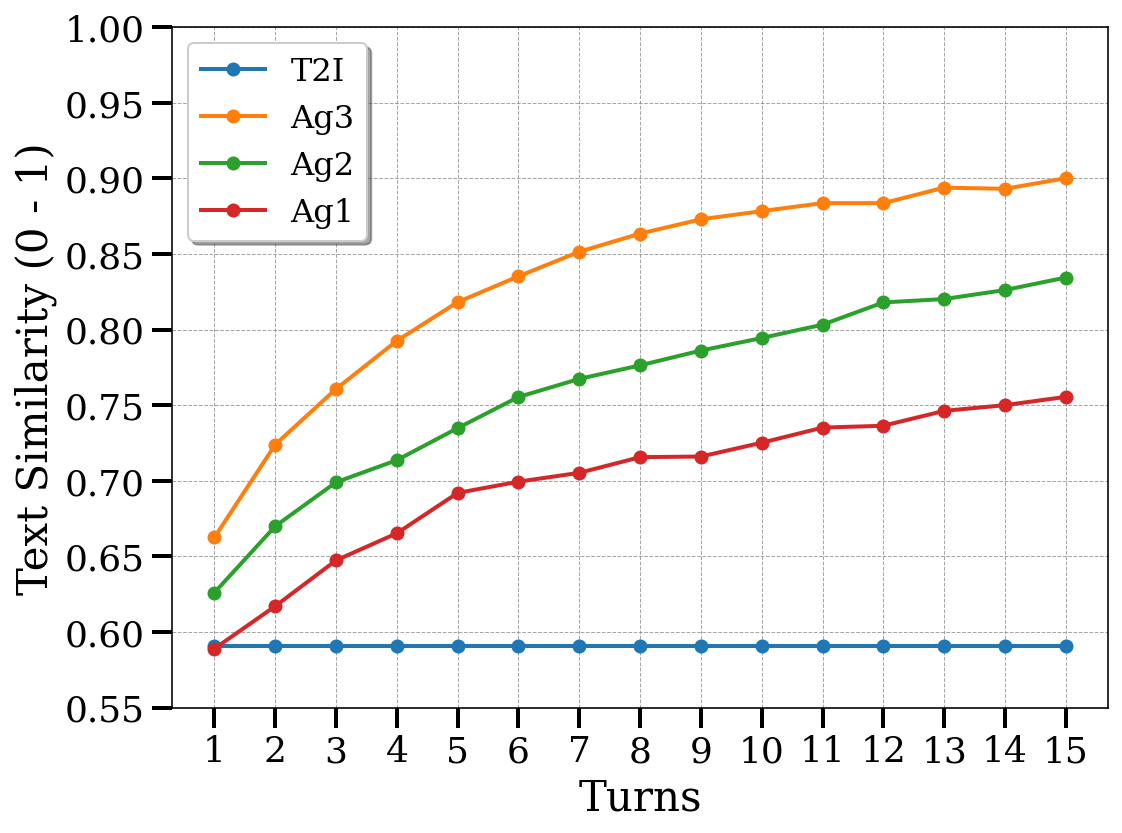
\includegraphics[width=\linewidth]{figures/coco_captions_dsgt2t.png}
  \end{minipage}
  \begin{minipage}{0.49\textwidth}
    \centering
    \textbf{DesignBench T2T DSG} 
    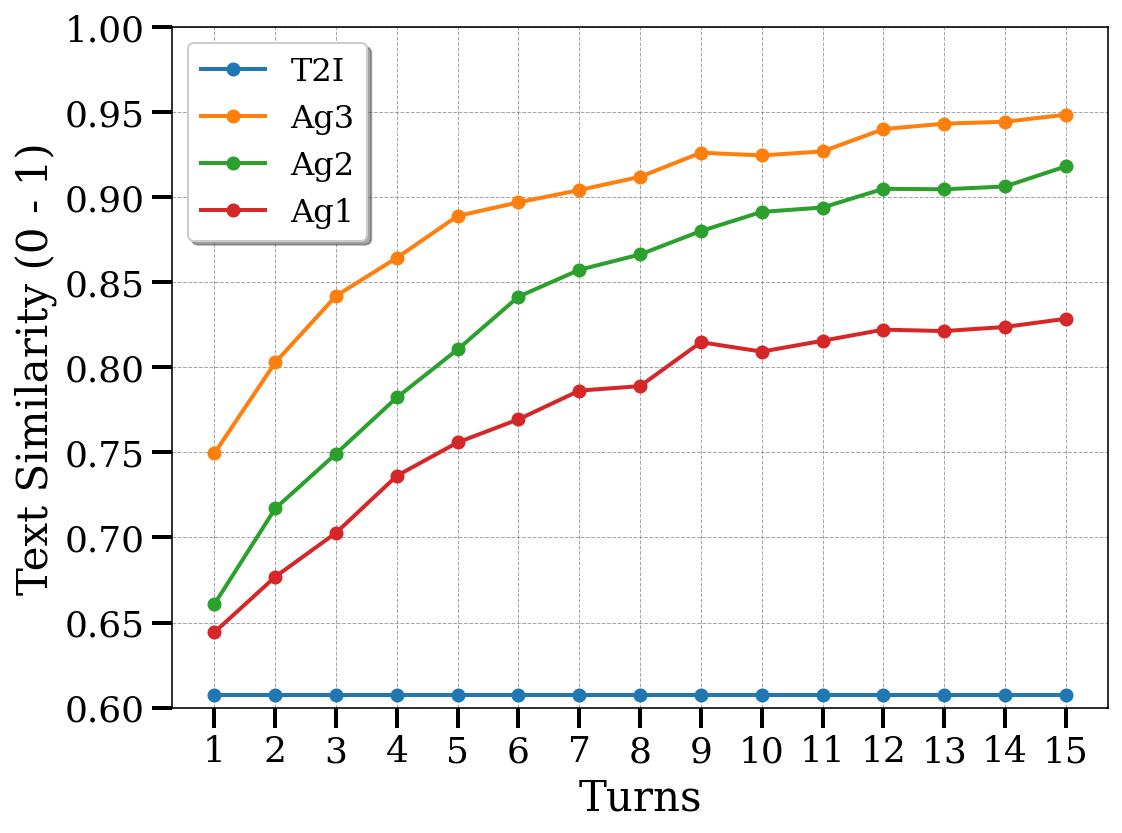
\includegraphics[width=\linewidth]{figures/toy_dataset_dsgt2t.png}
  \end{minipage}
  \caption{DSG score comparison between ground truth prompt and agent generated prompt reported at each turn. The performance of all agents increase with increase in number of turns.}
  \label{fig:dsg_figures}
\end{figure}


\begin{algorithm}[t]
\caption{User-Agent Self-Play Algorithm \nitkan{we can make this half page and wrap text around this. Not sure how, can someone try this?}}
\label{alg:converse_algo}
\begin{algorithmic}[1] 
\STATE \textbf{Input:} Initial prompt $p_0$, User $u$, Agent $a$ (with $p_0$), $max\_turns$
\STATE \textbf{Output:} Refined prompt $p_f$ 
\STATE $p_f \gets p_0$ 
\FOR{$turn\_id = 0$ \TO $max\_turns - 1$}
    \STATE $action \gets a.\text{SelectAction}()$
    \STATE $question \gets a.\text{VerbalizeAction}(action)$
    \STATE $answer \gets u.\text{AnswerQuestion}(question)$
    \STATE $a.\text{Transition}(action, answer)$
    \STATE $p_f \gets a.prompt$
\ENDFOR
\RETURN $p_f$
\end{algorithmic}
\end{algorithm}


\section{Details on the agent interface}

\label{app:interface}


Below is a showcase of how users could interact with the belief graph and clarifications in a hypothesised interface, to better iterate their inputs, to reach higher a quality and satisfaction of outputs. This is a crudely hypothesised, intentionally simple interface for the sake of research, but could be iterated and improved upon in many ways depending on application and users. 

\textbf{1. Default state}
On load of the app, there would be a text prompt input and space for output images, as is common across typical T2I interfaces. There would also be space for the user to view either clarifications from the model, or a graph interface, as part of the overall ``input'' section as these would act as a further input for future model output iterations. See \Cref{fig:interface1} below as reference. 

\begin{figure} [ht!]
    \centering
    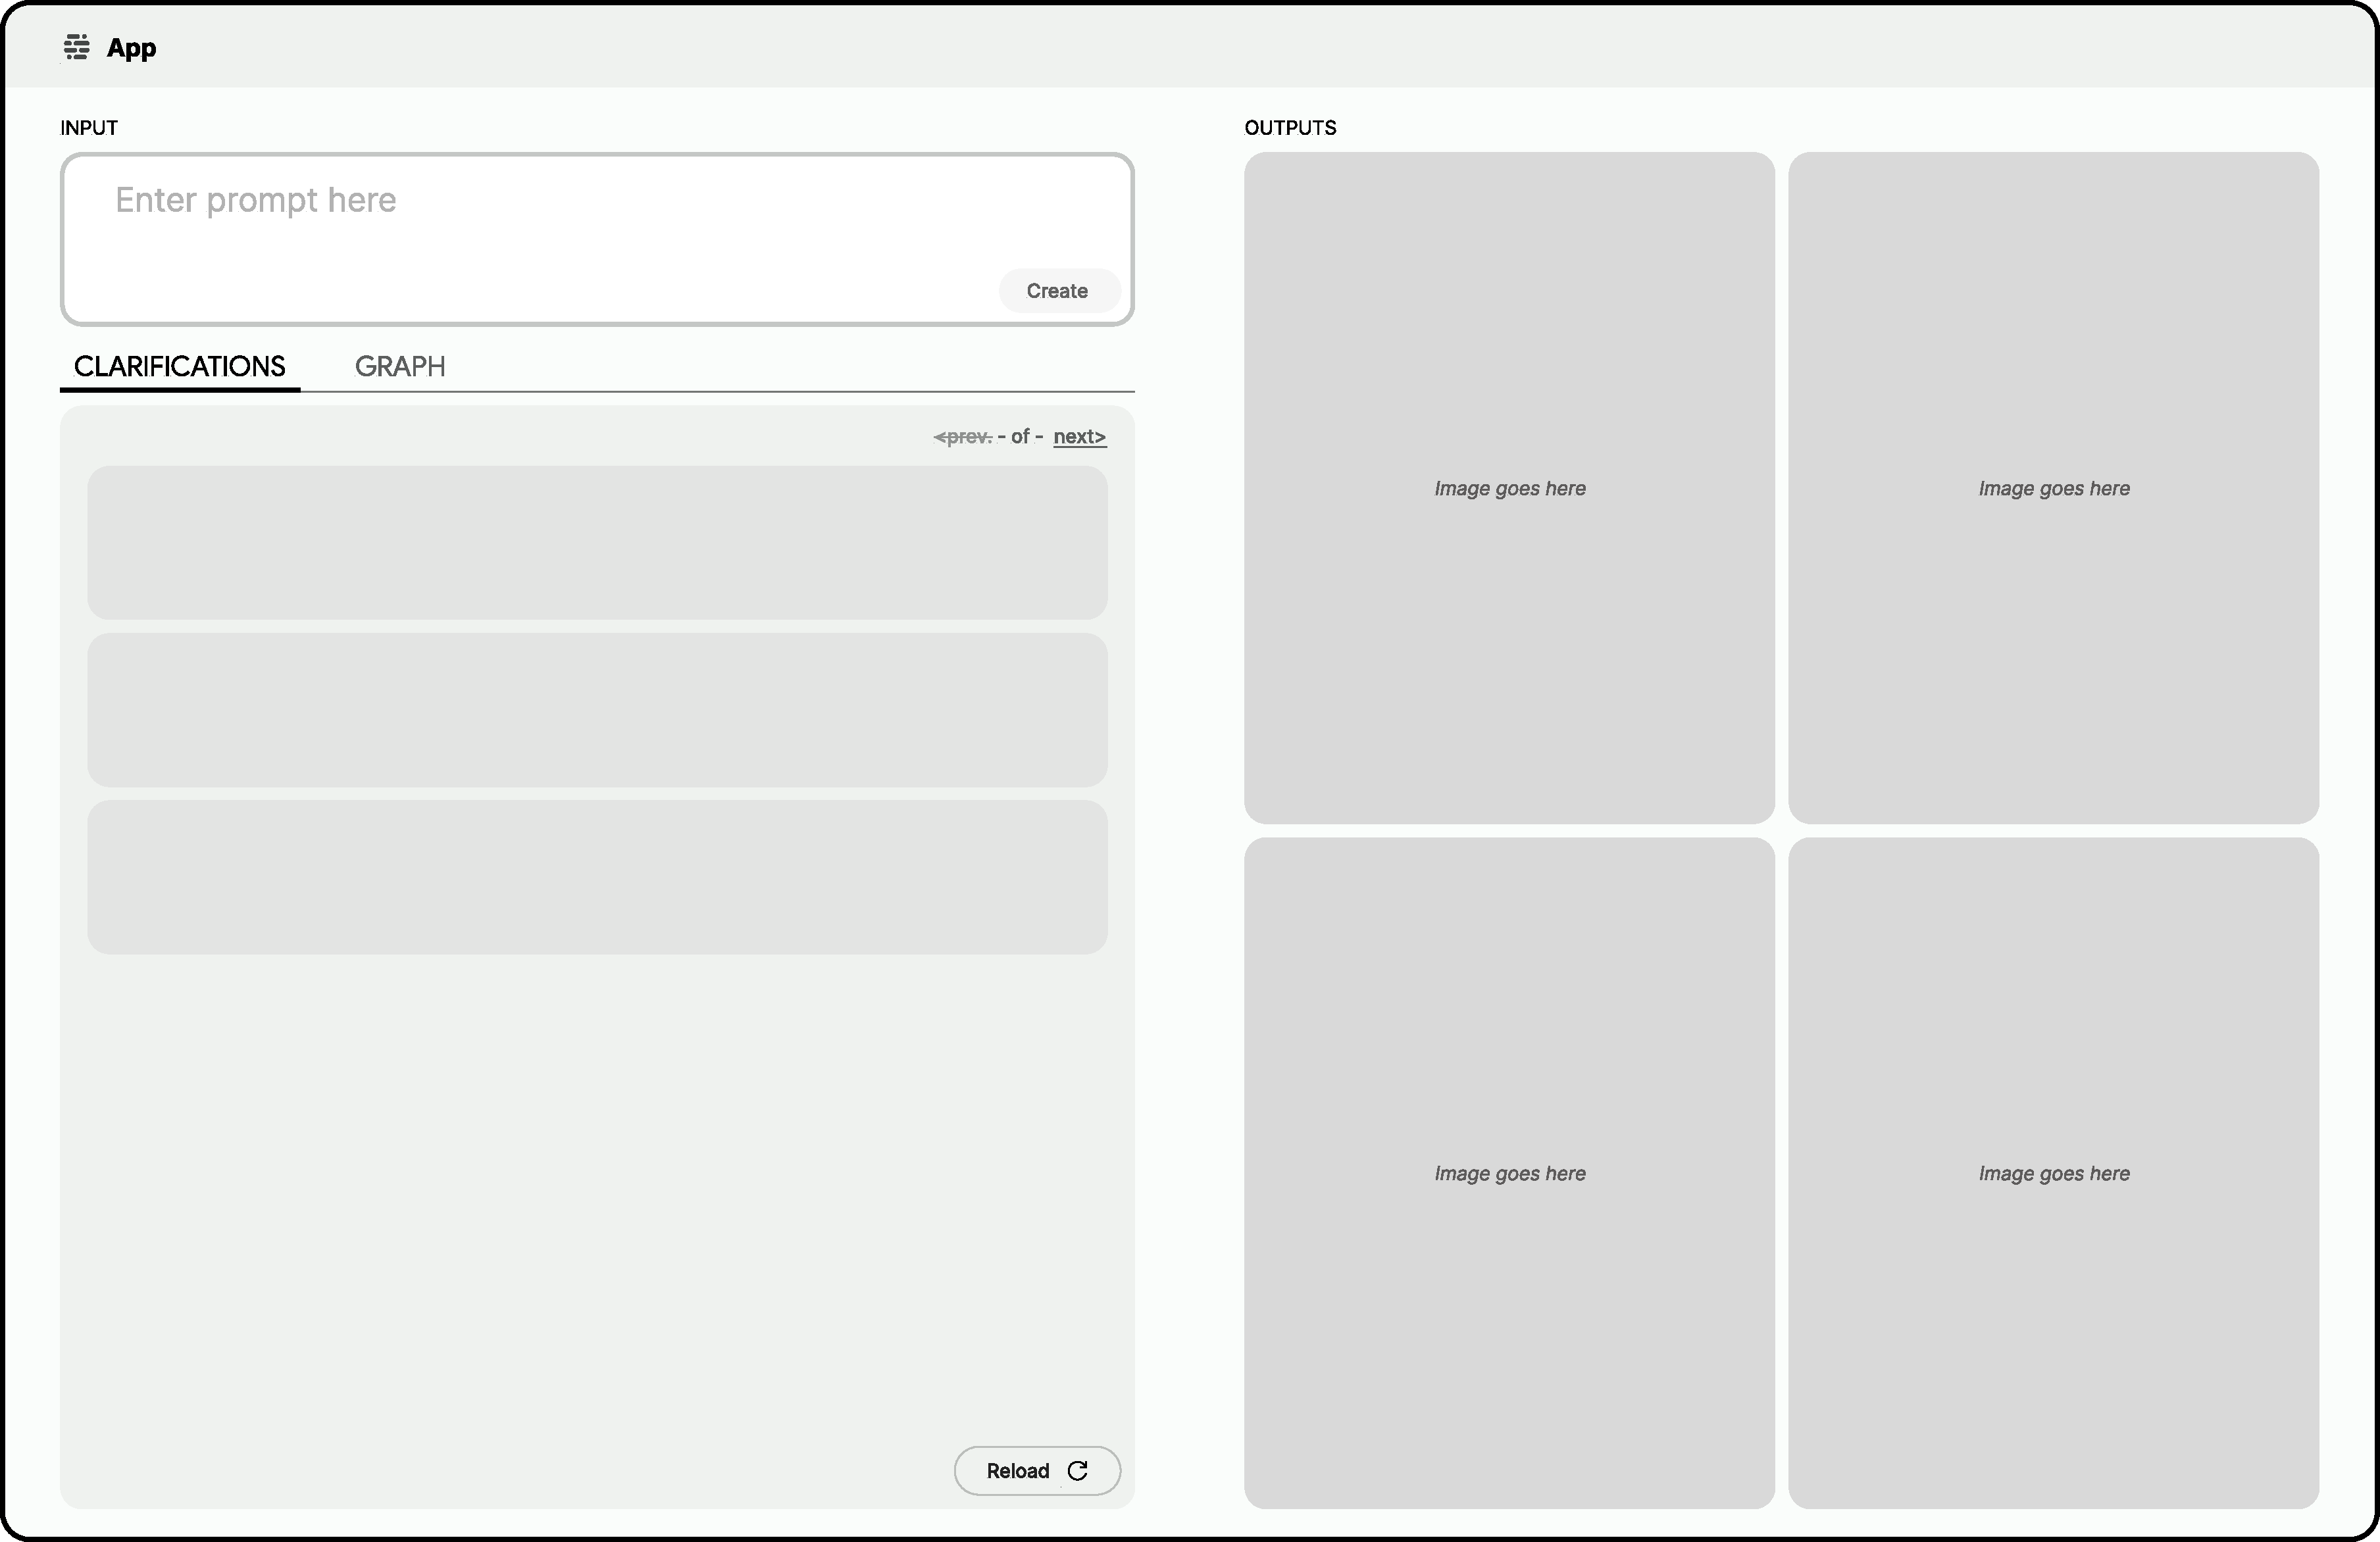
\includegraphics[width=.9\linewidth]{figures/Default.pdf}
    \caption{Default state of a possible interface.}
    \label{fig:interface1}
\end{figure} 

\textbf{2. Output images, with Clarifications} 
Once the user has submitted the prompt and the model has responded, there would be a set of images, as initial outputs from the users prompt. Below the input prompt would be a set of ``Clarifications'' in its populated state. These clarifications would ask the user specific questions that would be necessary to increase the specificity of the prompt, for the model to get a more accurate results aligned to the users intention, or to help the user realise their intention. Options would be given of the highest probability options for each Clarification, but the user could also fill in a totally new option via a free text field. Once answered by selection or text input, the clarifications would be added to the above, primary prompt for regeneration when the user selects. See \Cref{fig:interface2} below as reference.

\begin{figure} [ht!]
    \centering
    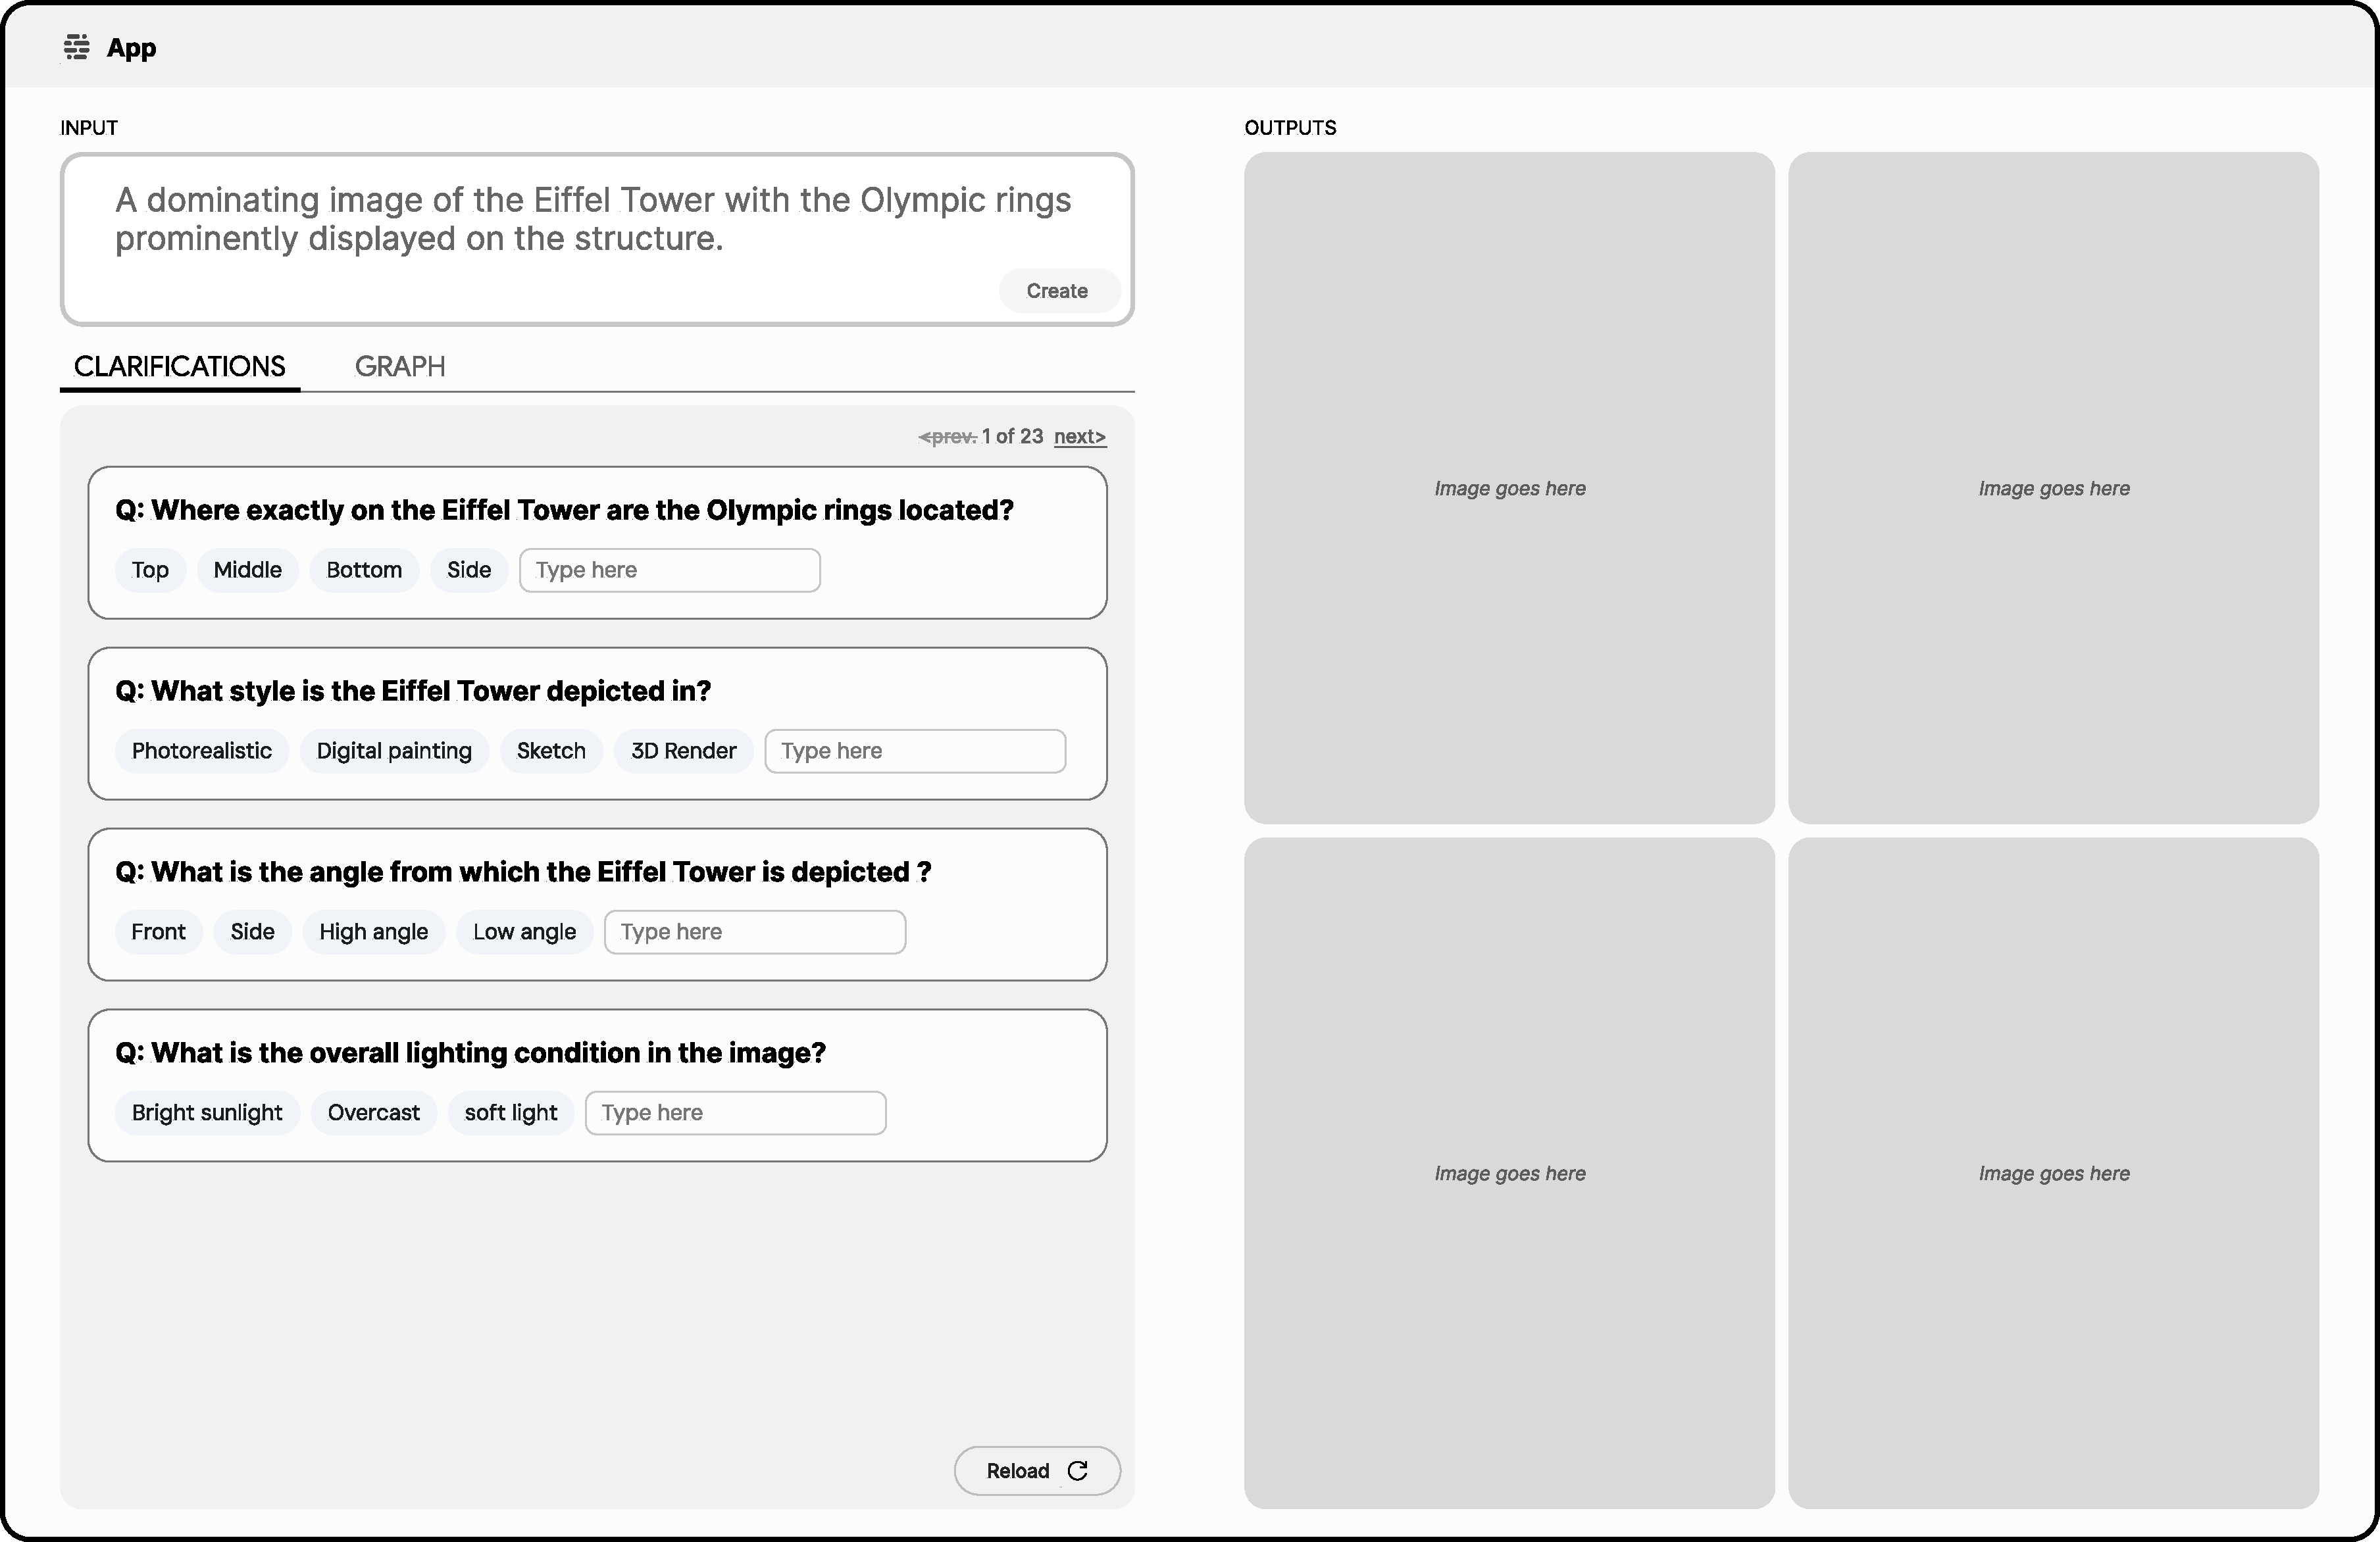
\includegraphics[width=.9\linewidth]{figures/Clarifications.pdf}
    \caption{Interface once prompt has been input with clarifications.}
    \label{fig:interface2}
\end{figure} 

\textbf{3. Graph Entities \& Attributes }
Instead of the clarifications, the user could select to instead view a Graph by clicking  Tab above the clarifications themselves. This graph would  be populated will all Entities from the prompt explicit and implicit visually defined differently (in this diagram by the dotted line surrounds implicit entities, but is a filled line when surrounding explicit entities). The graph layout will be structured, depicting relationships concentrically i.e. "on", "in" or "under" for example, will become child entities, and be displayed within the parent entities' boundary. For example a 'Mug' that has the relationship of 'on' a 'Table' entity, will sit within the boundary of 'Table', as also would a 'Plate' if that had the same child-parent relationship. 

Below the Graph would also be a list of 'cards' (i.e. boxed groups of information), one for each "explicit" or "implicit" entity. Within each card a user could see the status of implicit / explicit, and change this status to confirm or deny its presence. The user could also see a list of "attributes" associated to that entity, which the model has assumed. Each of these attributes could be changed by interacting with a list of alternatives via drop down. These lists are determined in terms of which items and order of items, based on the probability by which the model sees them, ordered with higest first. This probability would be made clear to the user to define the order by seeing the peercentage next to the label. See \Cref{fig:interface3} below as reference.

\begin{figure} [ht!]
    \centering
    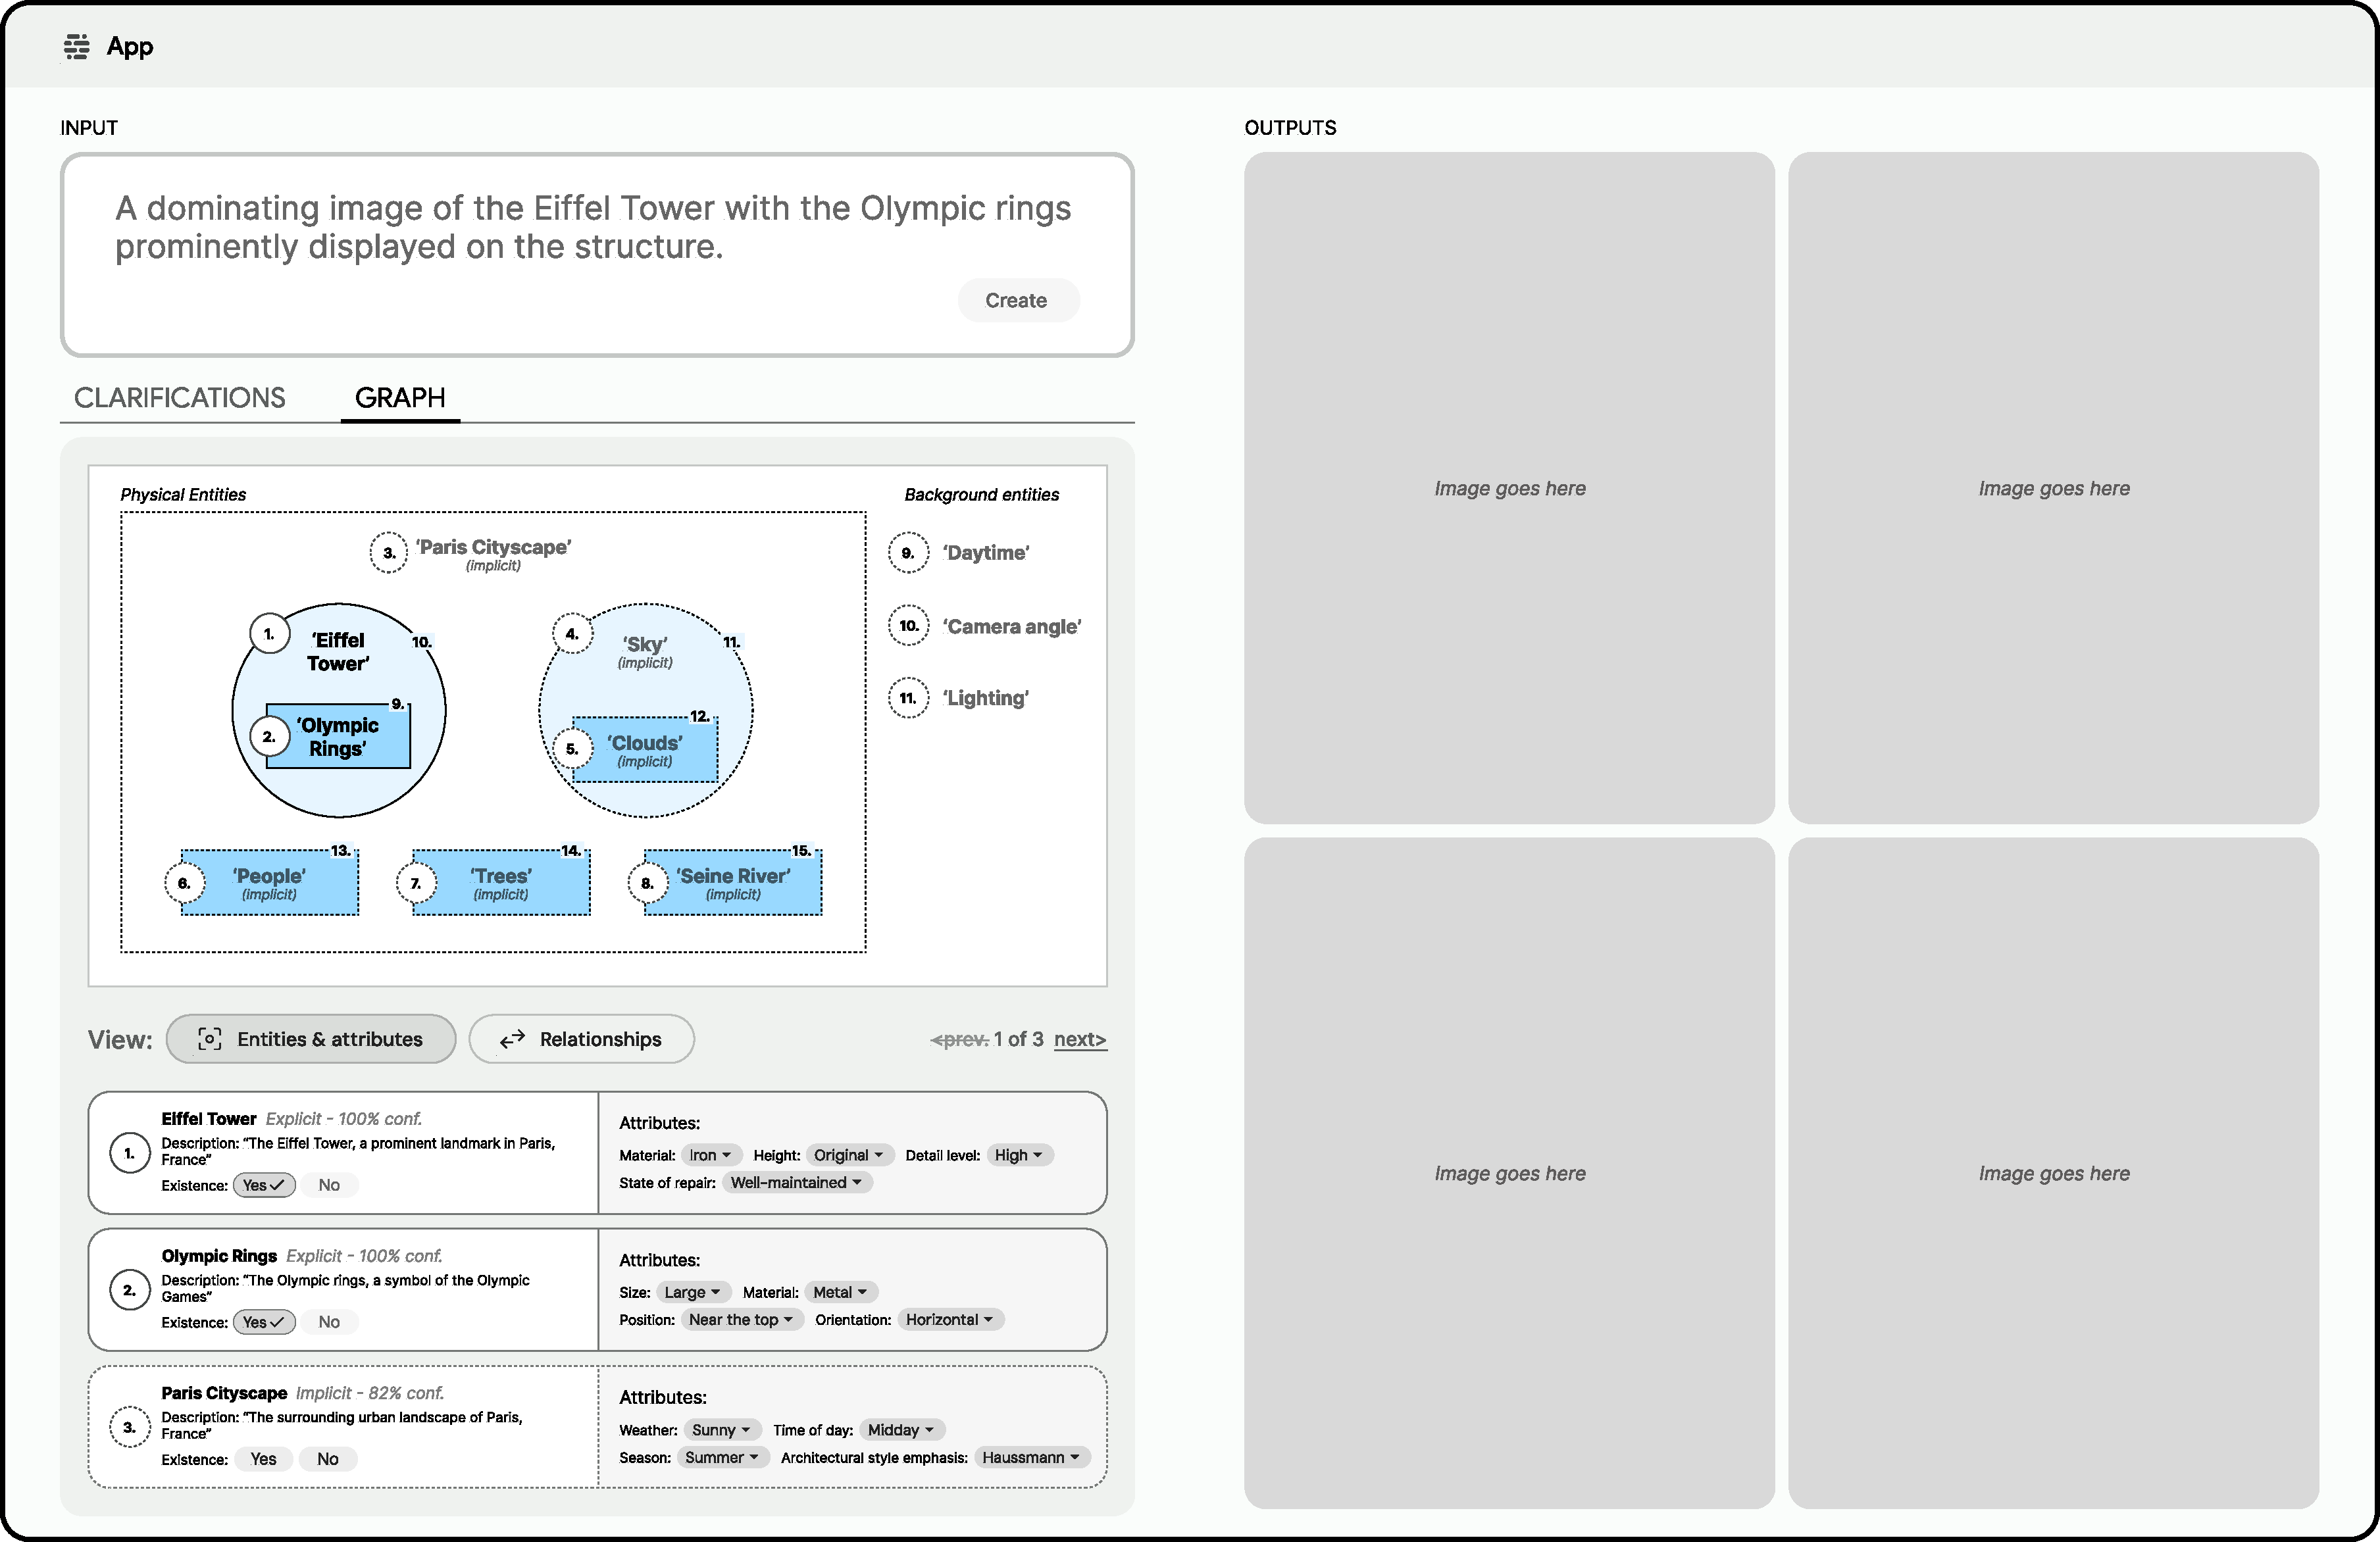
\includegraphics[width=.9\linewidth]{figures/Attributes.pdf}
    \caption{Interface with Graph displaying Entities, with cards below enabling a user to change attributes associated to each entity.}
    \label{fig:interface3}
\end{figure} 

\textbf{4. Graph Relationships} 
The user would also be able to change the state of the Graph and Cards, to instead focus on the relationships between entities, by toggling to "Relations". In this state the user would be able to focus on two specific entities (e.g. 'mug' and 'table'), see the description of the relationship (e.g. 'the mug is sitting on the table') and if desired change the relationship to an alternative (e.g. 'on', changed to 'under') via a drop down of options which the model determined as alternative options ordered by probability, as per attributes. See Figure \Cref{fig:interface4} below as reference.

\begin{figure} [ht!]
    \centering
    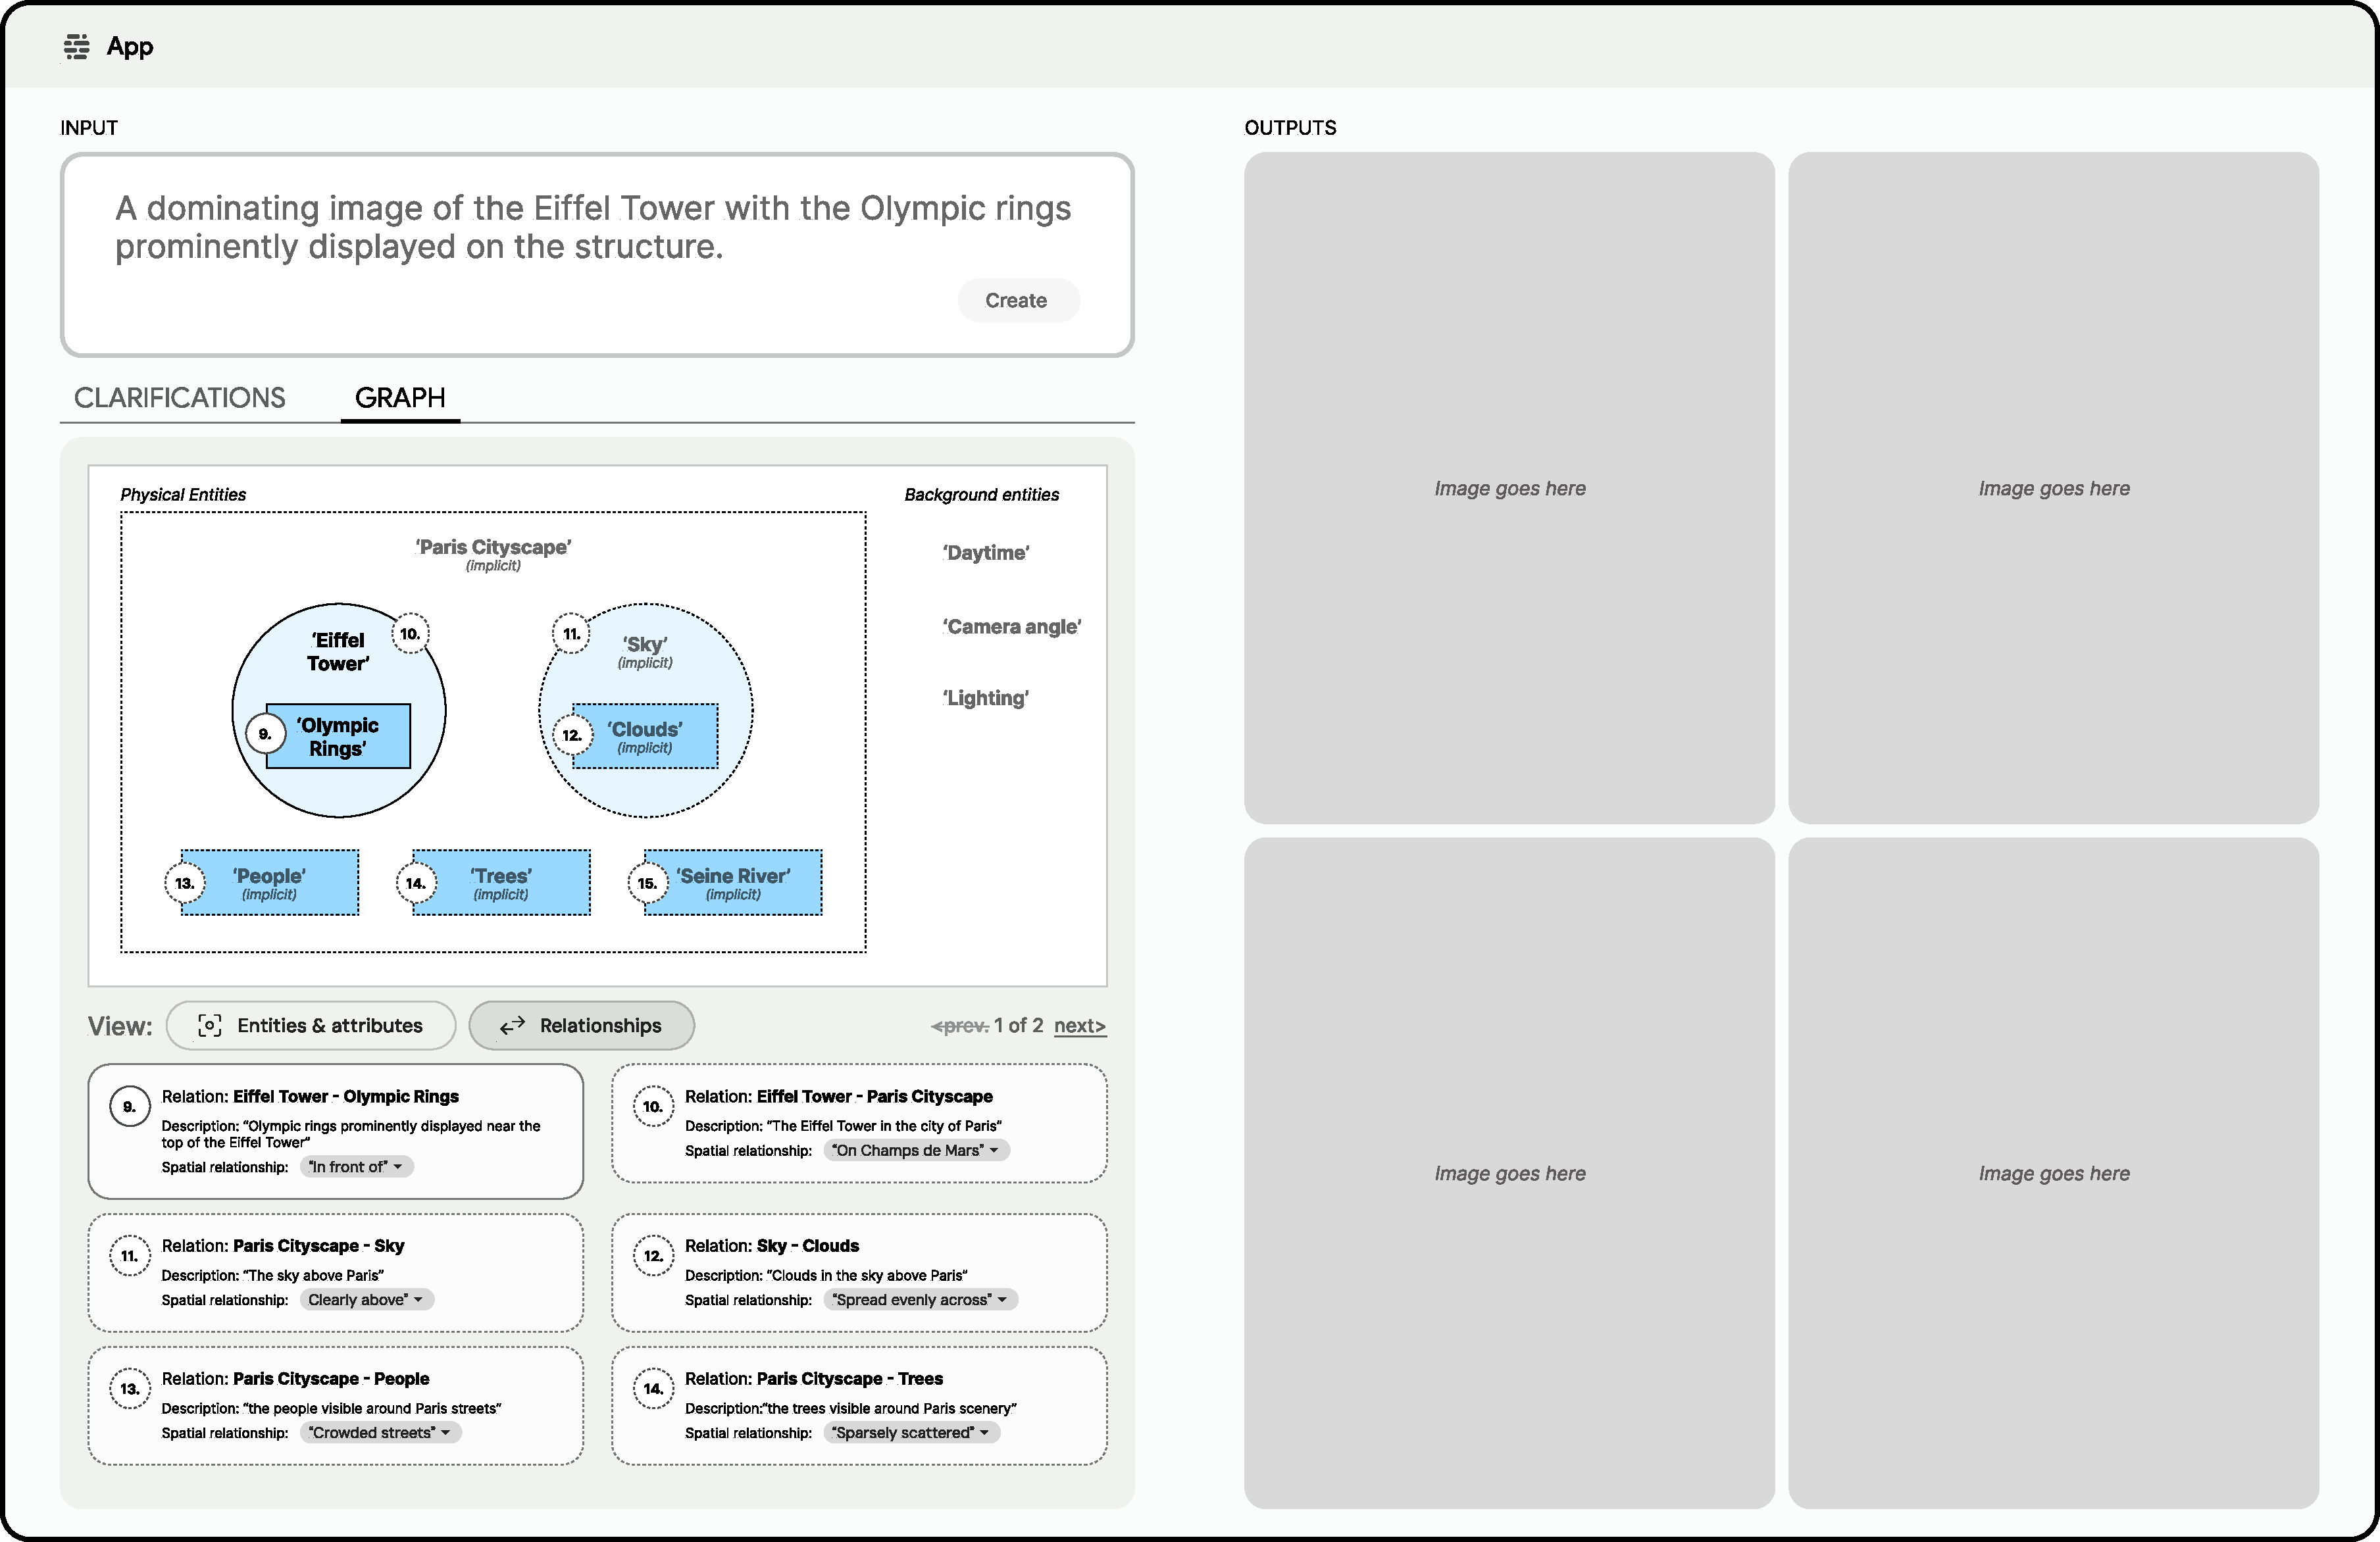
\includegraphics[width=.9\linewidth]{figures/Relations.pdf}
    \caption{Interface with Graph displaying relations between Entities, with cards below enabling a user to change relationships between entities.}
    \label{fig:interface4}
\end{figure} 

Once any of these changes are made the user could initiate a regeneration via the updated prompt to create a new set of output images, which can then be further refined via the same method. 


\section{Details on user studies for the agent interface}
\label{user_study}
Below we describe the exact guideline definitions we shared with the user for a user study.

\subsubsection{Hypothesized Frustrations}
We presented participants with the following hypothesized frustrations related to T2I model usage:
\begin{enumerate}
\item \textbf{Prompt Misinterpretation:} The model misunderstands complex relationships between entities in the input prompt.
\item \textbf{Many Prompt Iterations:} The model does not immediately generate what the user intends, requiring numerous iterative changes to the input prompt.
\item \textbf{Inconsistent Generations:} The model reinterprets the input prompt differently between iterations, causing unwanted changes in the generated images.
\item \textbf{Incorrect Assumptions:} The model makes incorrect assumptions or no assumptions when encountering gaps in the details provided in the input prompt, leading to undesired outputs.
\end{enumerate}

Explanations of terms were given to users of: 
\begin{enumerate}
\item "Entities" are single items that are intended to be in the image e.g. "Cat" and "Ball", from "make a sketch of a Cat playing with a Ball"
\item "Prompt" means the text written to communicate the intended output image e.g. the sentence "make a sketch of a Cat playing with a Ball" is the "Prompt", also known as "Input" 
\item "Iterations" are each set of different image outputs by the model, taken from a different input, or even the same input just regenerated
\end{enumerate}

The question asked for each Frustration were: "Please score the below frustrations (or issues) that could be related to Text to Image AI Generation"."Rank in terms of how much they relate to your current usage, with your most commonly used model or app." 




\subsubsection{Hypothesized Features}
We proposed the following features as potential solutions to address the identified frustrations:
\begin{enumerate}
\item \textbf{Clarifications:} The model would ask specific clarifying questions about uncertainties in the prompt.  These details would then be incorporated into subsequent iterations. For example: "Is the cat playing with: 1. a ball of wool, or 2. a tennis ball?"
\item \textbf{Graph of Prompt Entities:}  A visual representation of all entities in the prompt as a graph, allowing users to see and edit attributes of each entity.  E.g., seeing that the model has assigned "round," "small," and "wooden" as attributes to "table" and allowing the user to change them to "square" and "metal."
\item \textbf{Graph of Prompt Relationships:} A visual representation of relationships between entities in the prompt, allowing users to see and edit these relationships. E.g., seeing that "donut" is "next to" "coffee" and allowing the user to change the relationship to "on top of."
\end{enumerate}

The questions asked for each feature were: 
\begin{enumerate}
\item "How likely this feature is to help your current workflow if you had it now?". With response options of: "Very unlikely to help", "Unlikely to help", "Could help", "Likely to help", "Very likely to help". 
\item "How soon would this feature deliver value to your work?" with response options of: "Very soon / immediately", "Sometime, "Not very soon".
\end{enumerate}

Image references were given for each Feature as listed out below:

\begin{enumerate}
\item \textbf{Clarifications:} 
\begin{figure} [H]
    \centering
    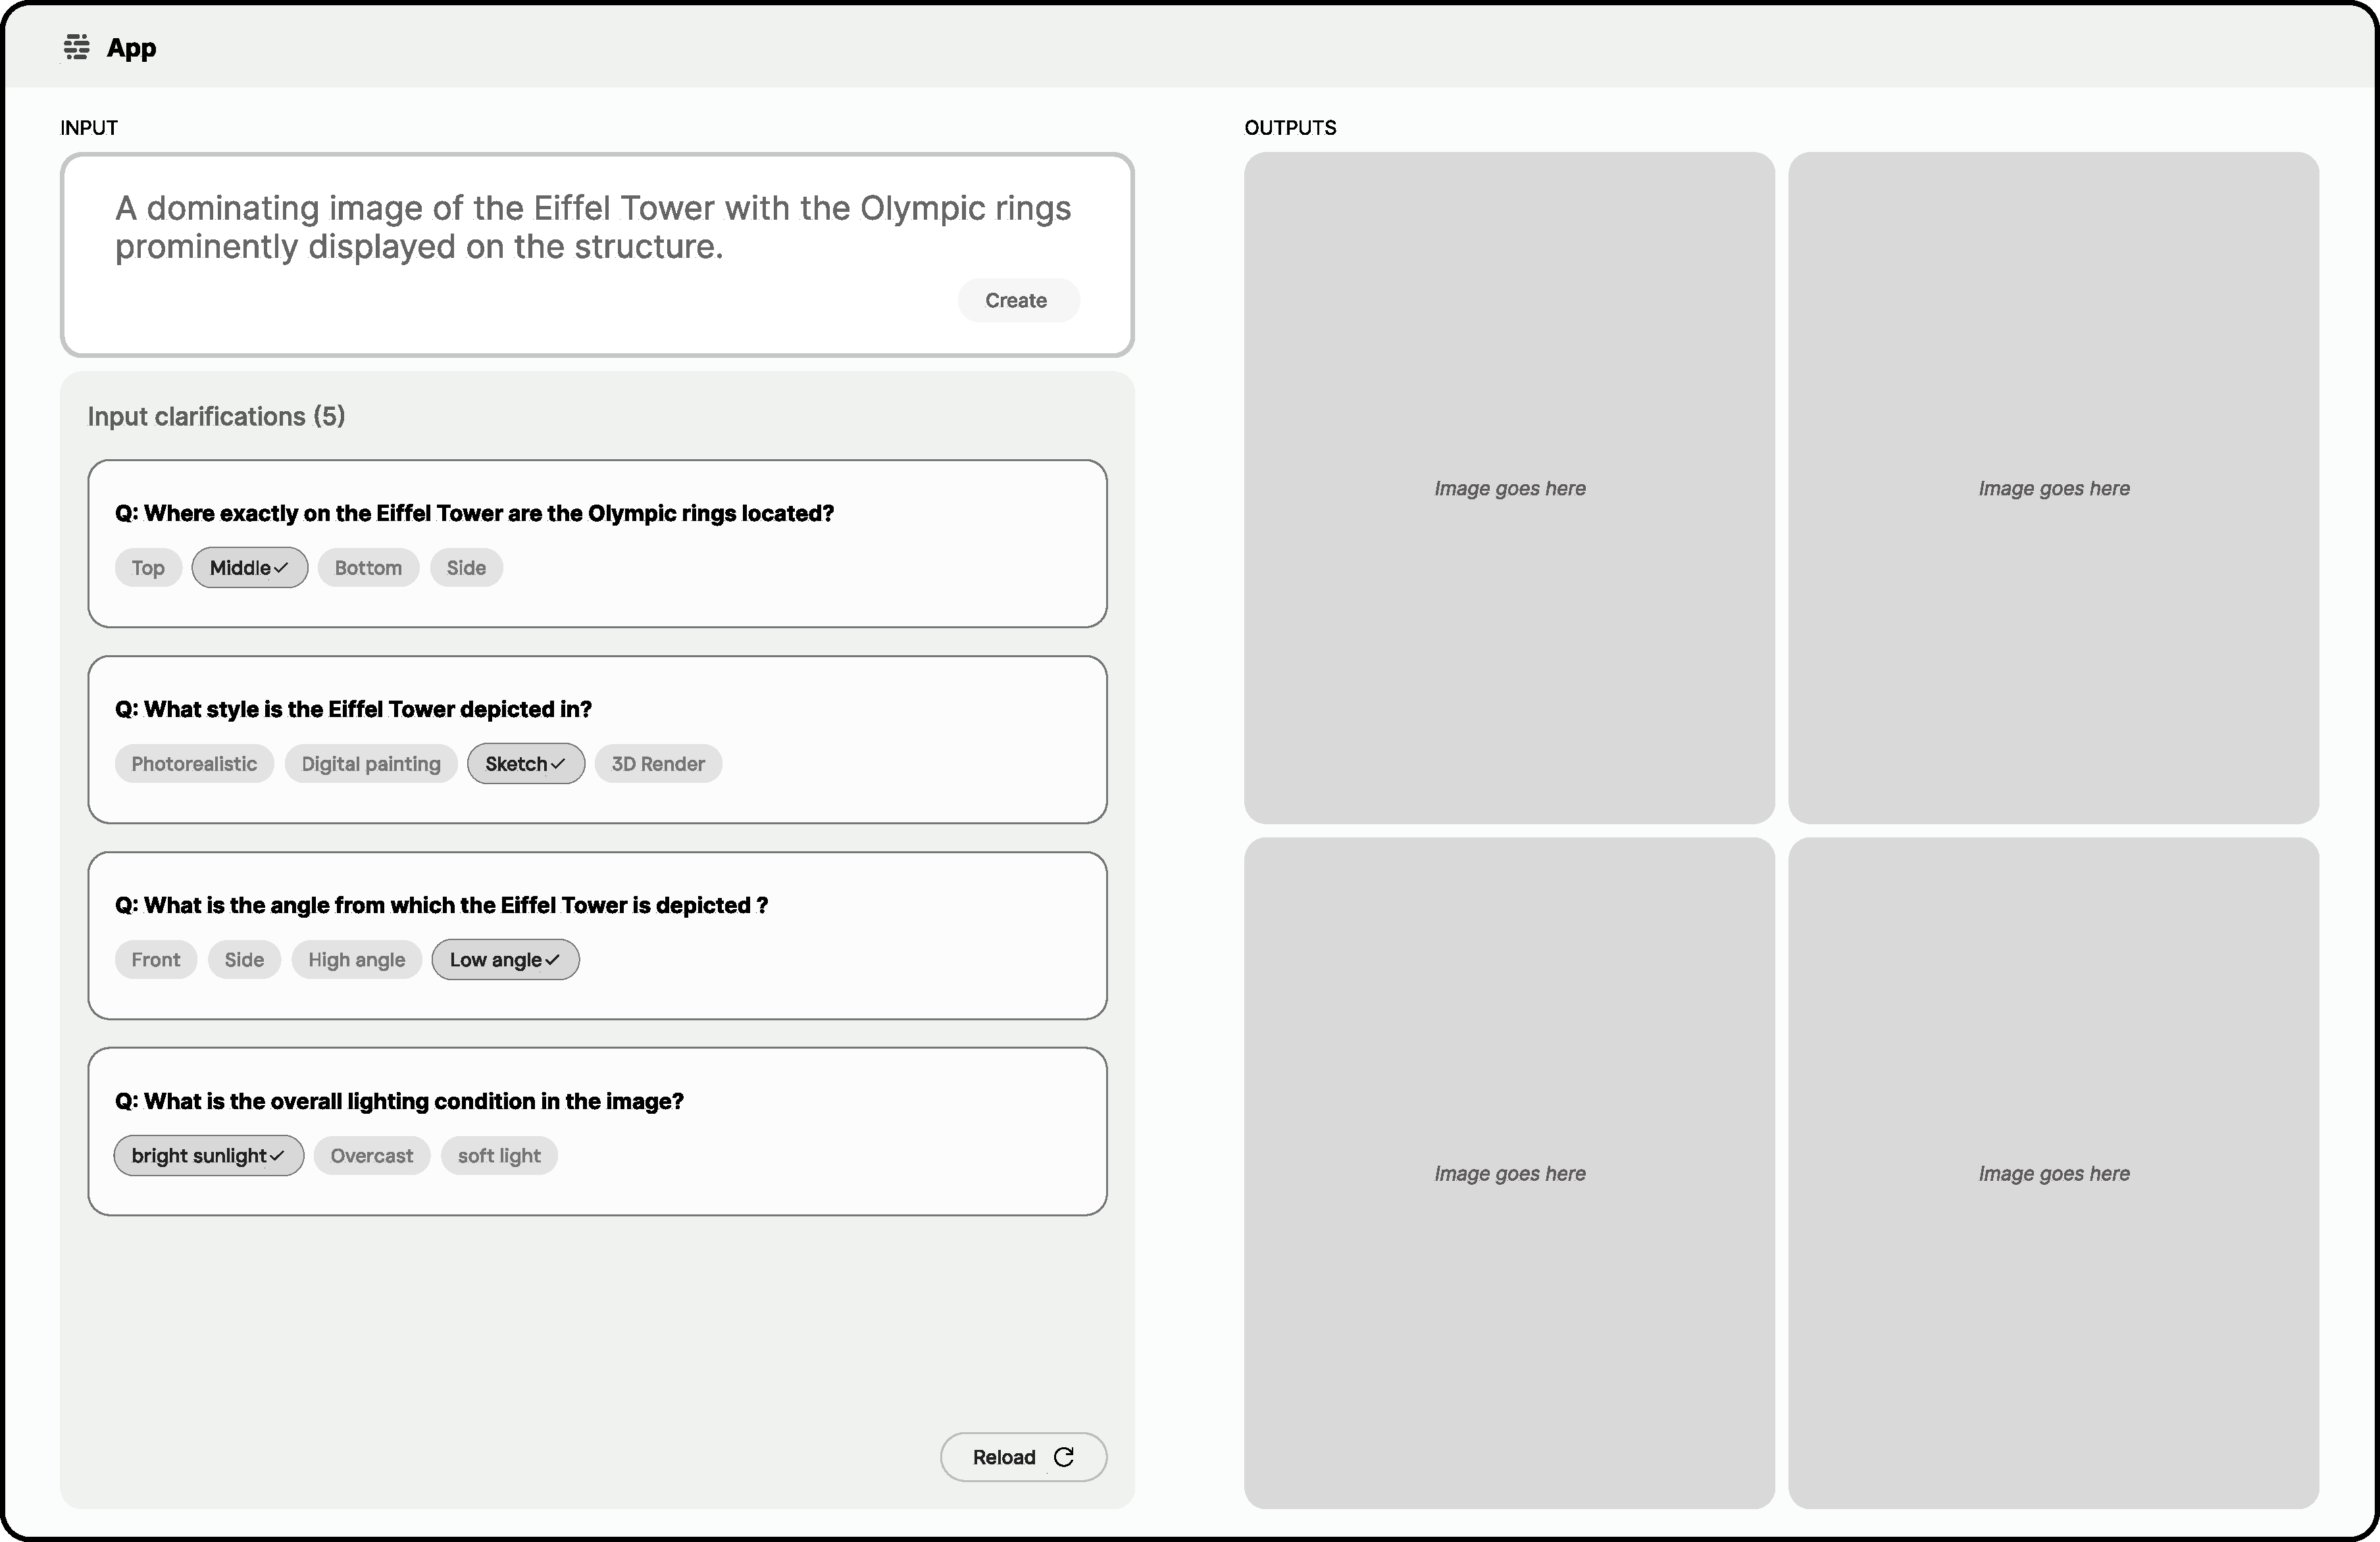
\includegraphics[width=.9\linewidth]{figures/F1_Questions.pdf}
    \caption{Stimulus image in the survey to test the Model clarifications feature.}
    \label{fig:interface-human}
\end{figure} 

\clearpage
\item \textbf{Graph of Prompt Entities:}  
\begin{figure} [H]
    \centering
    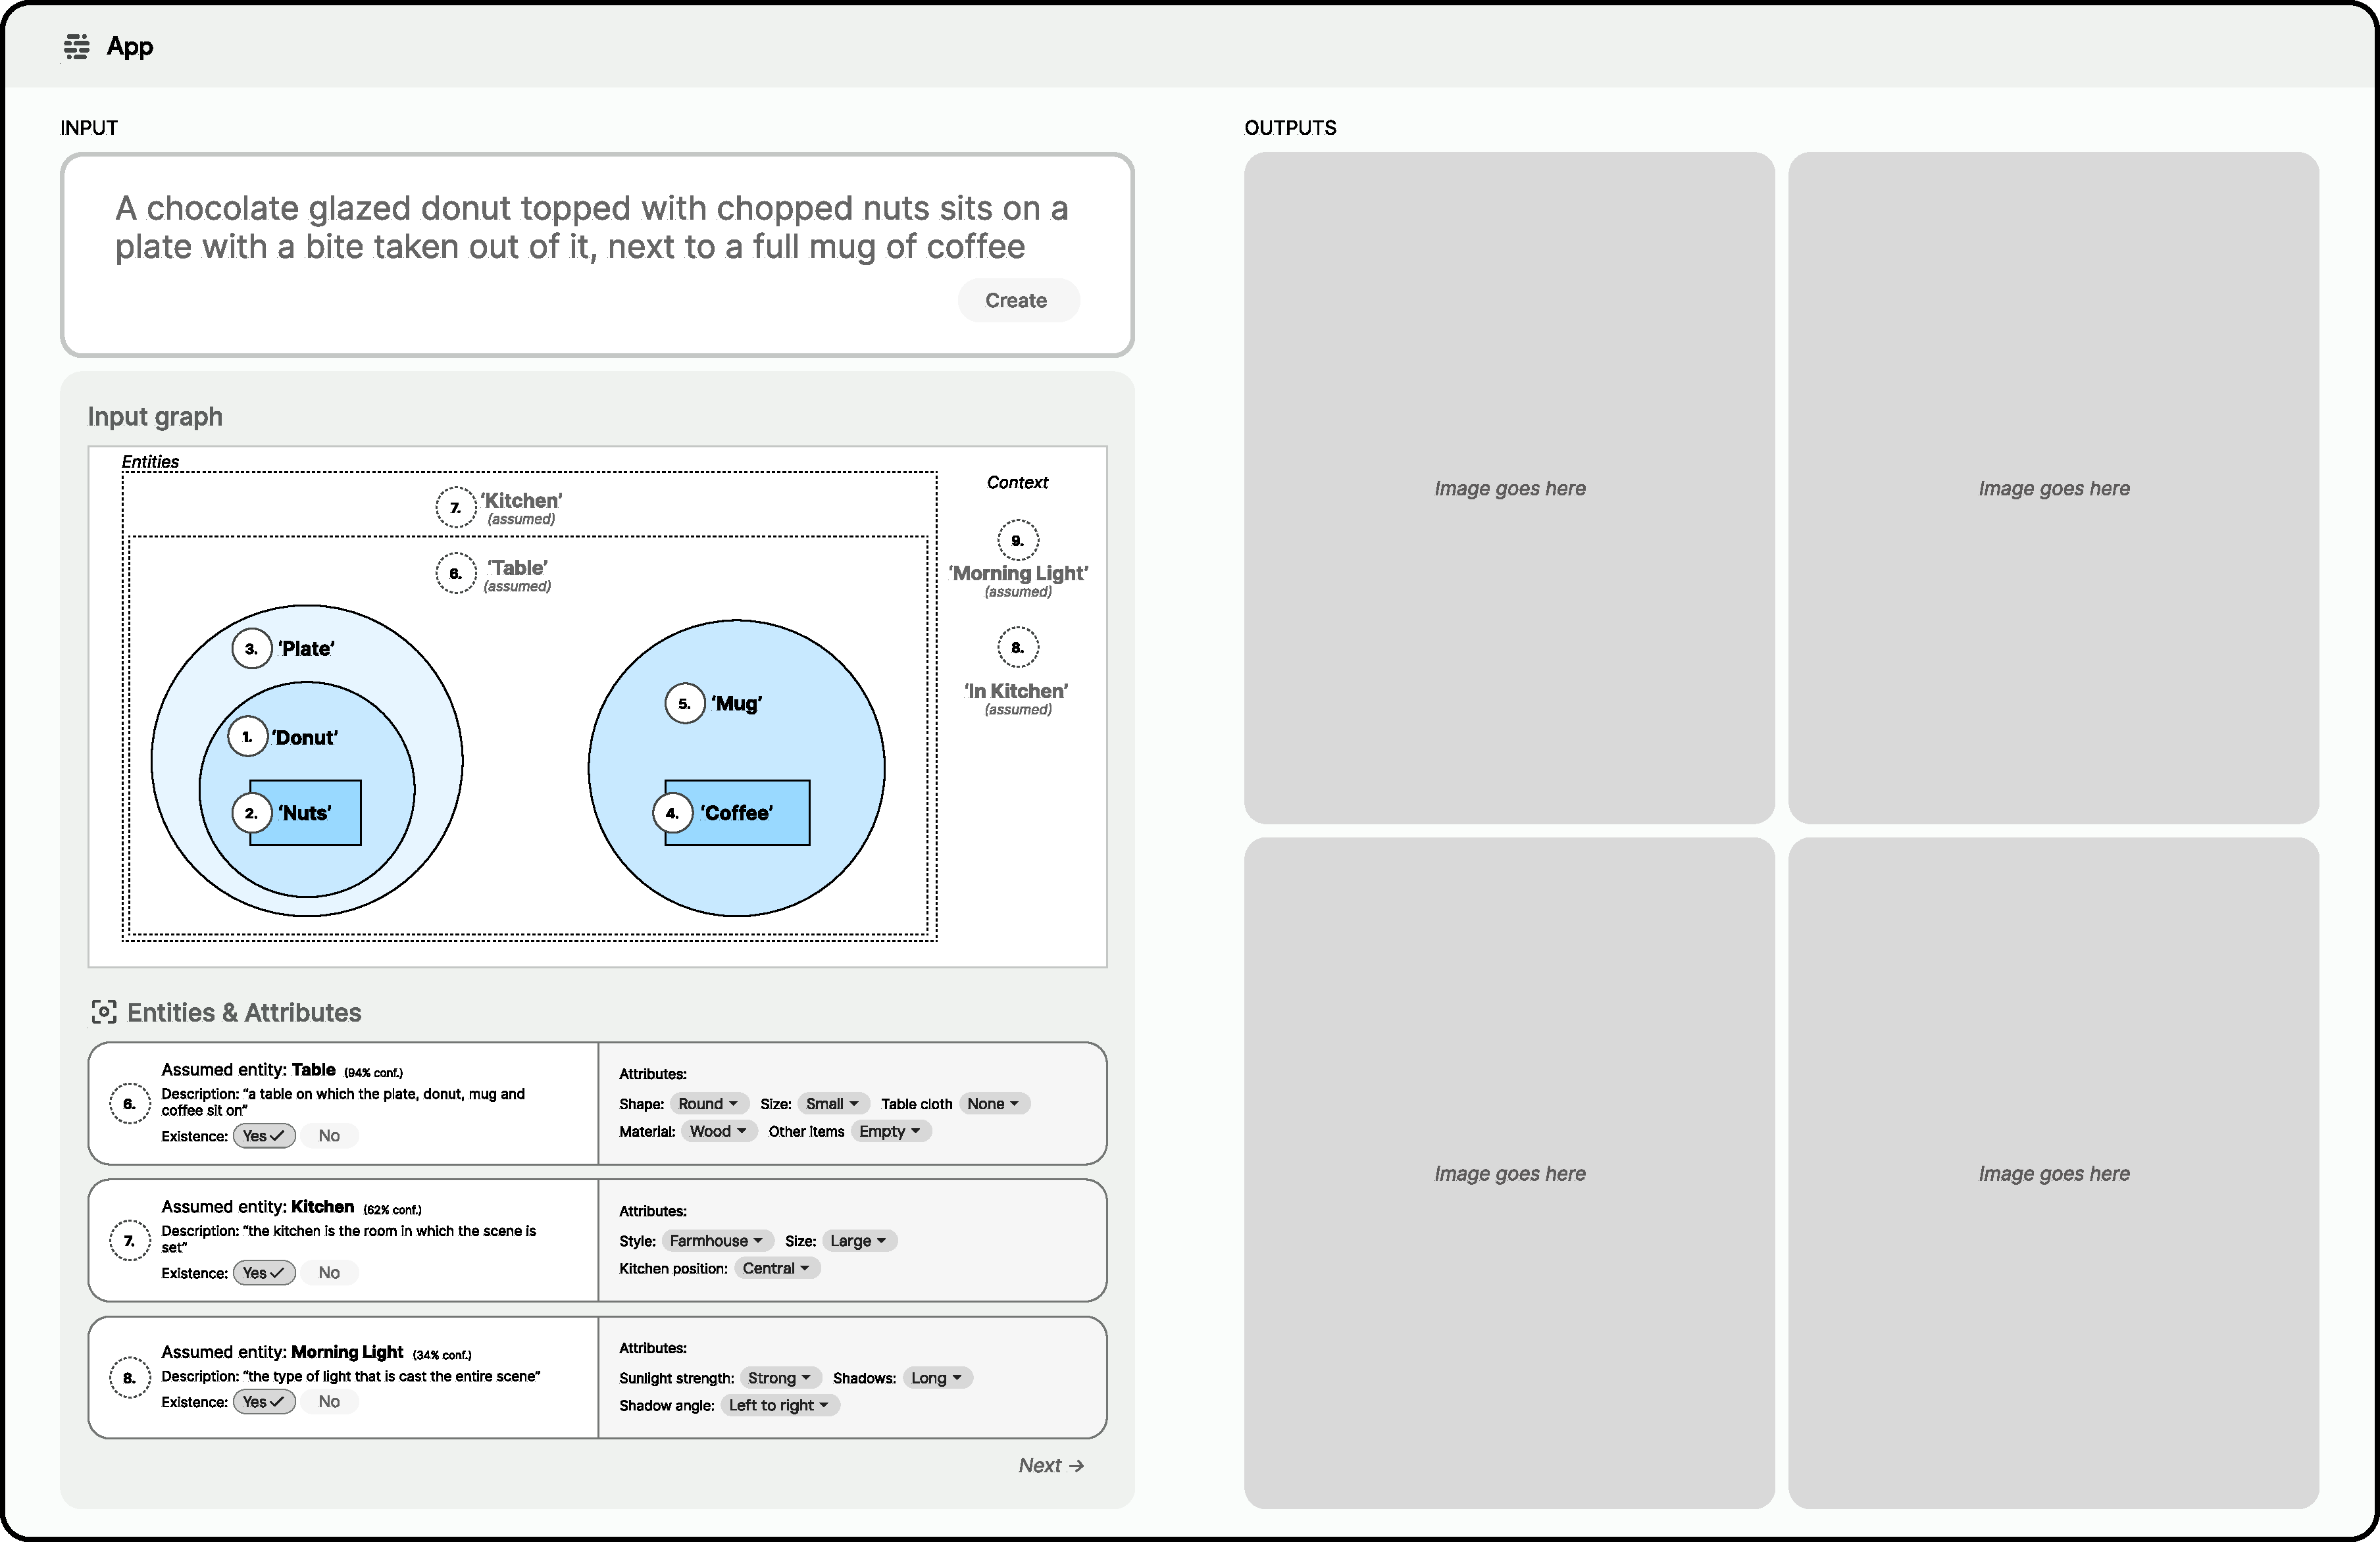
\includegraphics[width=.9\linewidth]{figures/F2_Graph.pdf}
    \caption{Stimulus image in the survey to test the Model Graph of Entities and Attributes feature.}
    \label{fig:interface-human2}
\end{figure} 

\item \textbf{Graph of Prompt Relationships:} 
\begin{figure} [H]
    \centering
    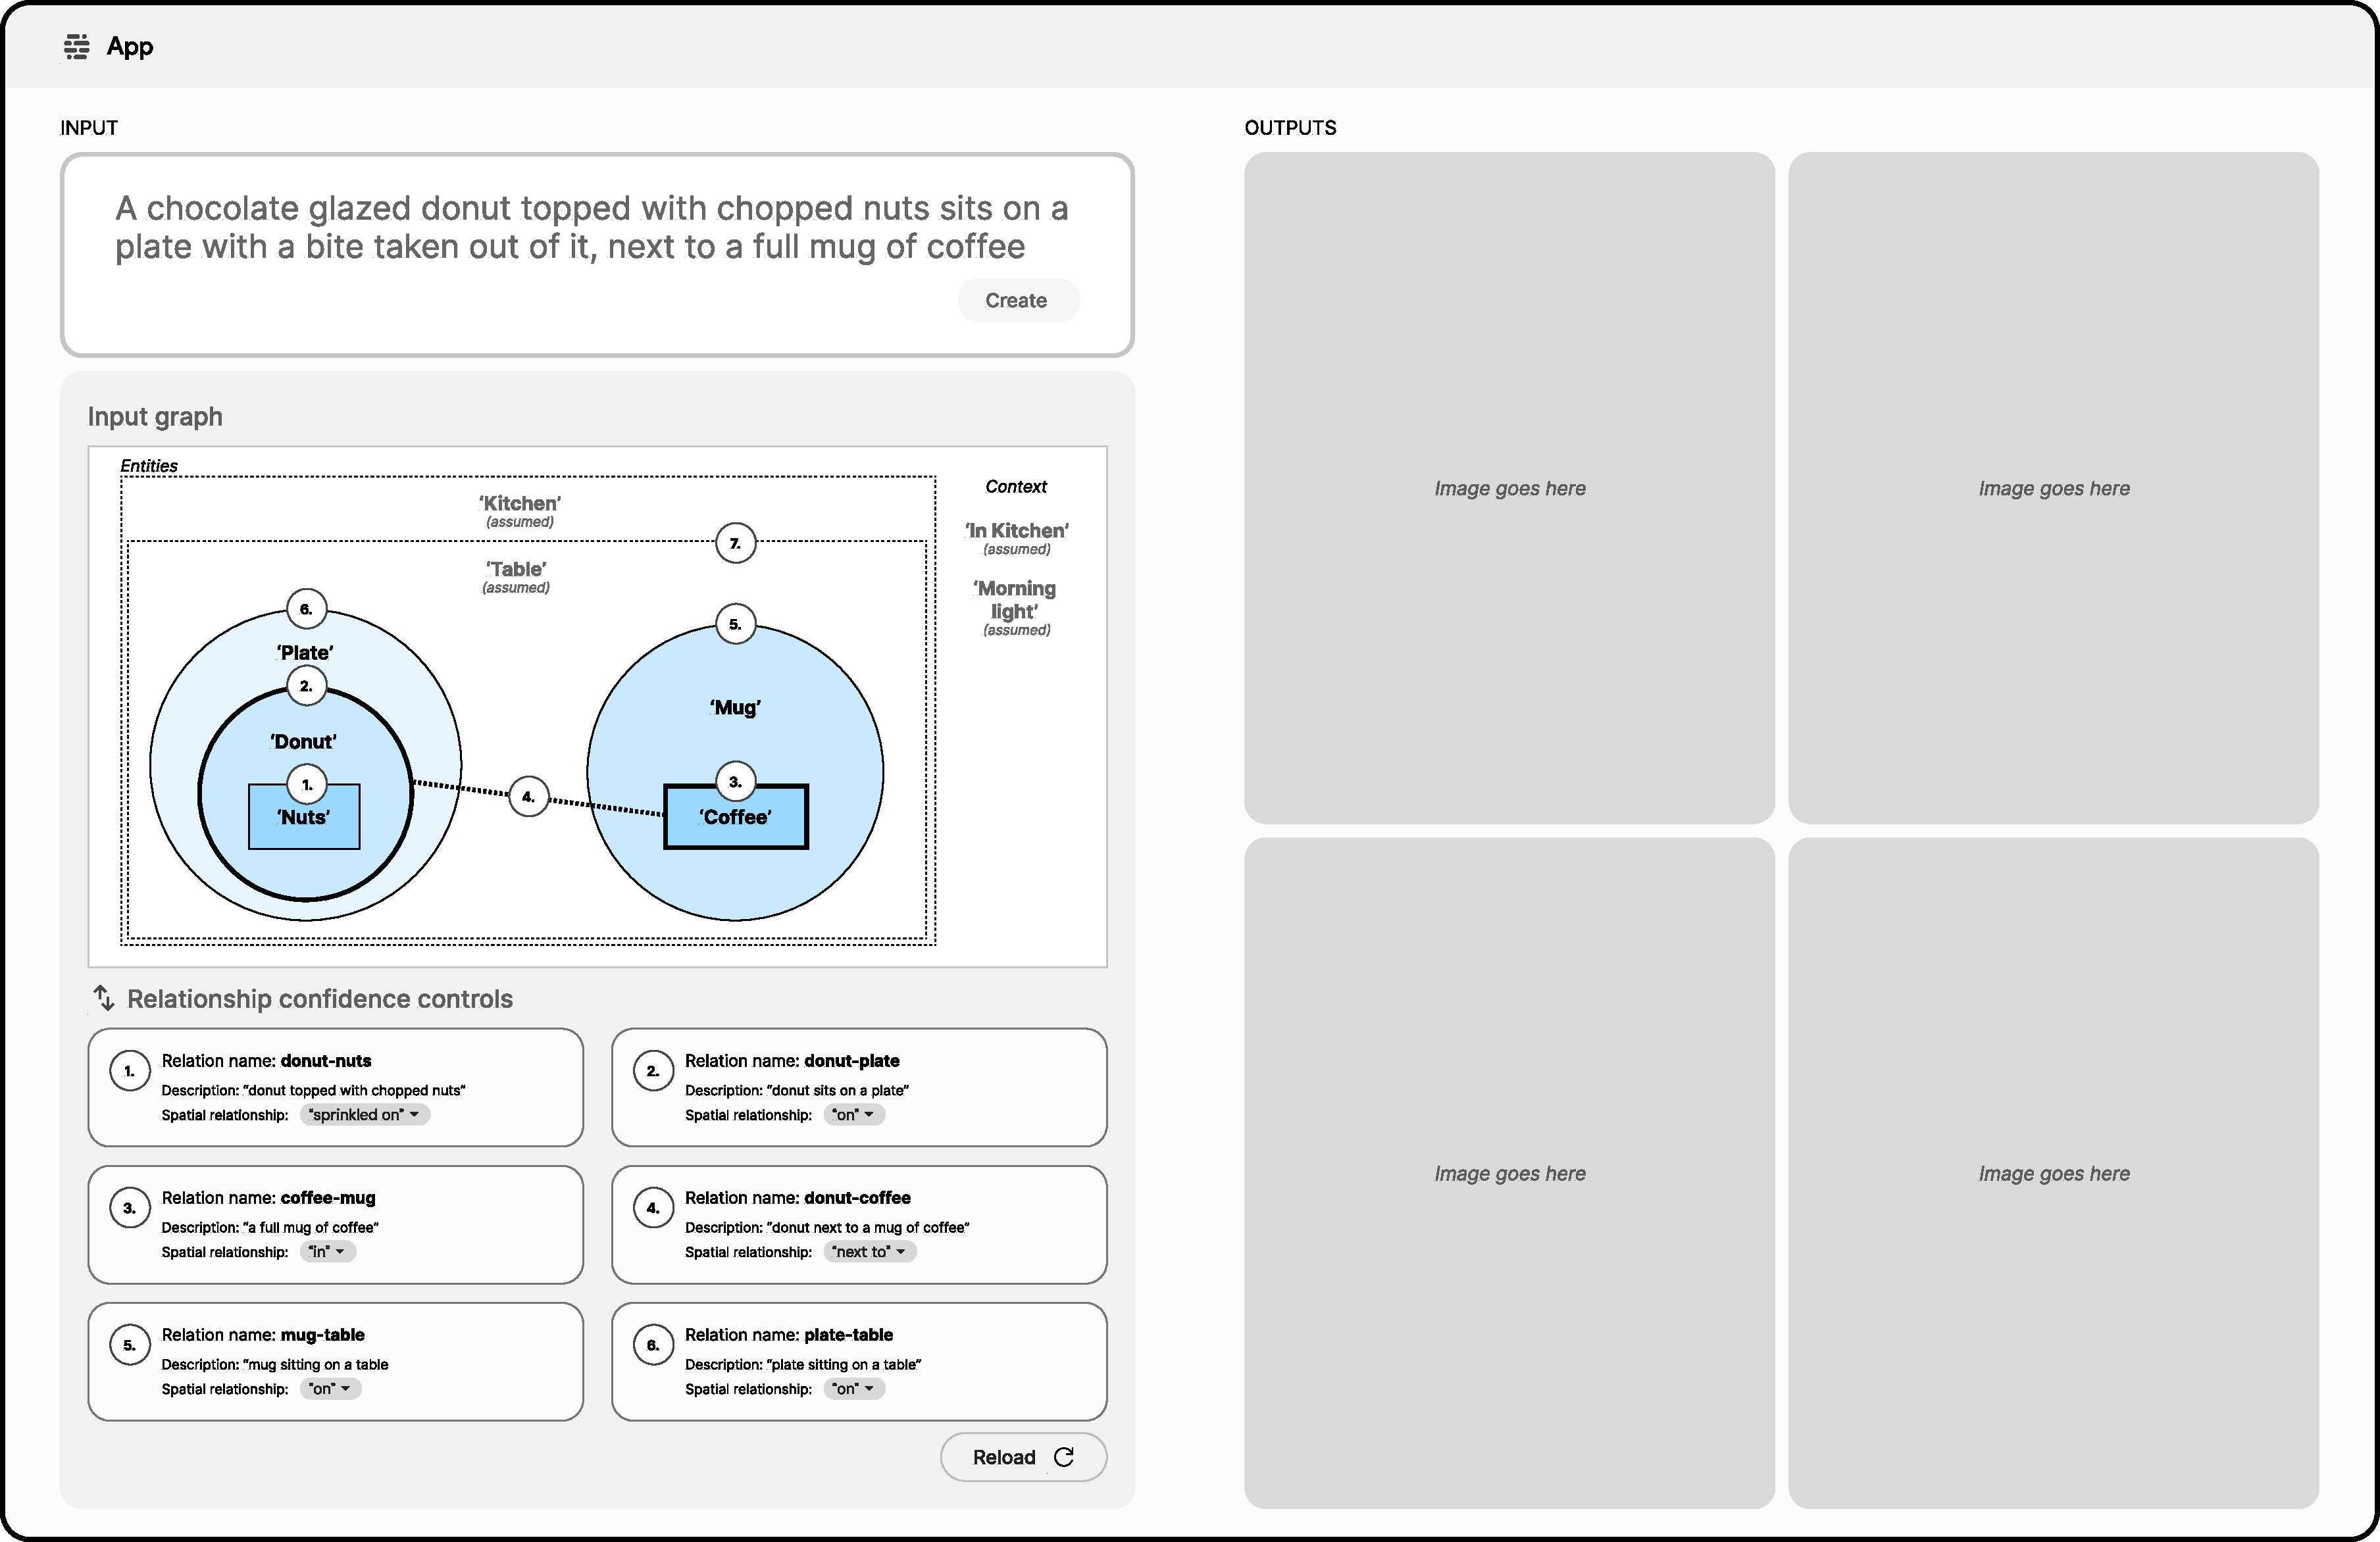
\includegraphics[width=.9\linewidth]{figures/F3_Relations.pdf}
    \caption{Stimulus image in the survey to test the Model Graph of Entity Relations feature.}
    \label{fig:interface-human3}
\end{figure} 

\end{enumerate}

\subsubsection{Human Study Results}
\Cref{tab:t2i_frequency} details the T2I usage frequency of the human subjects. \Cref{table_frustration1} shows the percentage of human subjects that reported different kinds of frustrations in their experience of using T2I. \Cref{table_frustration2} summarizes the results on expected speed of value delivered from different features of our agent prototypes. These results highlight the impact of our contributions.
\begin{table}[h]
\caption{Breakdown of the T2I usage frequency of the 143 participants recorded}
\centering
\label{tab:t2i_frequency}
\begin{tabular}{lrr} 
\toprule
\textbf{Usage Frequency} & \textbf{No. of participants} & \textbf{(\%)} \\
\midrule
Many times a day & 13 & 9.1 \\ 
Many times a week & 44 & 30.8 \\
At least once a week & 36 & 25.2 \\
At least once a month & 50 & 35.0 \\
\bottomrule
\end{tabular}
\end{table}


\begin{table}[h]
\caption{Reported User Frustrations with existing T2I processes (\% of participants)}
\centering
\small
\begin{tabular}{lccccc} %
\toprule
\textbf{Frustration} & \textbf{V. Freq. (\%)} & \textbf{Freq. (\%)} & \textbf{Occas. (\%)} & \textbf{V. Occas. (\%)} & \textbf{No Issue (\%)} \\ %
\midrule
Prompt Misinterpret. & 7 & 19.6 & 43.4 & 23.1 & 7 \\  %
Many Iterations & 10.5 & 44.8 & 28 & 11.9 & 4.9 \\ %
Inconsistent Gen. & 11.2 & 20.3 & 39.9 & 21 & 7.7 \\ %
Incorrect Assumptions & 7 & 23.1 & 39.2 & 20.3 & 10.5 \\ %
\bottomrule
\end{tabular}
\label{table_frustration1}  %
\end{table}


\begin{table}[h]
\caption{Expected speed of value delivered from features (\% of users)}
\centering
\small
\begin{tabular}{lccccc} %
\toprule
\textbf{Feature} & \textbf{Very soon / immediately (\%)} & \textbf{Sometime(\%)} & \textbf{Not very soon. (\%)}
\\ %
\midrule
Clarifications & 57.7 & 37.2 & 5.1 \\  %
Entity Graph & 49.6 & 34.8 & 15.6 \\ %
Relation Graph & 41.8 & 44 & 14.2 \\ %
\bottomrule
\end{tabular}
\label{table_frustration2}  %
\end{table}


\clearpage
\textbf{Template of Human Rater Task 1: Evaluation of Issues in Individual Questions} 
\begin{figure} [H]
    \centering
    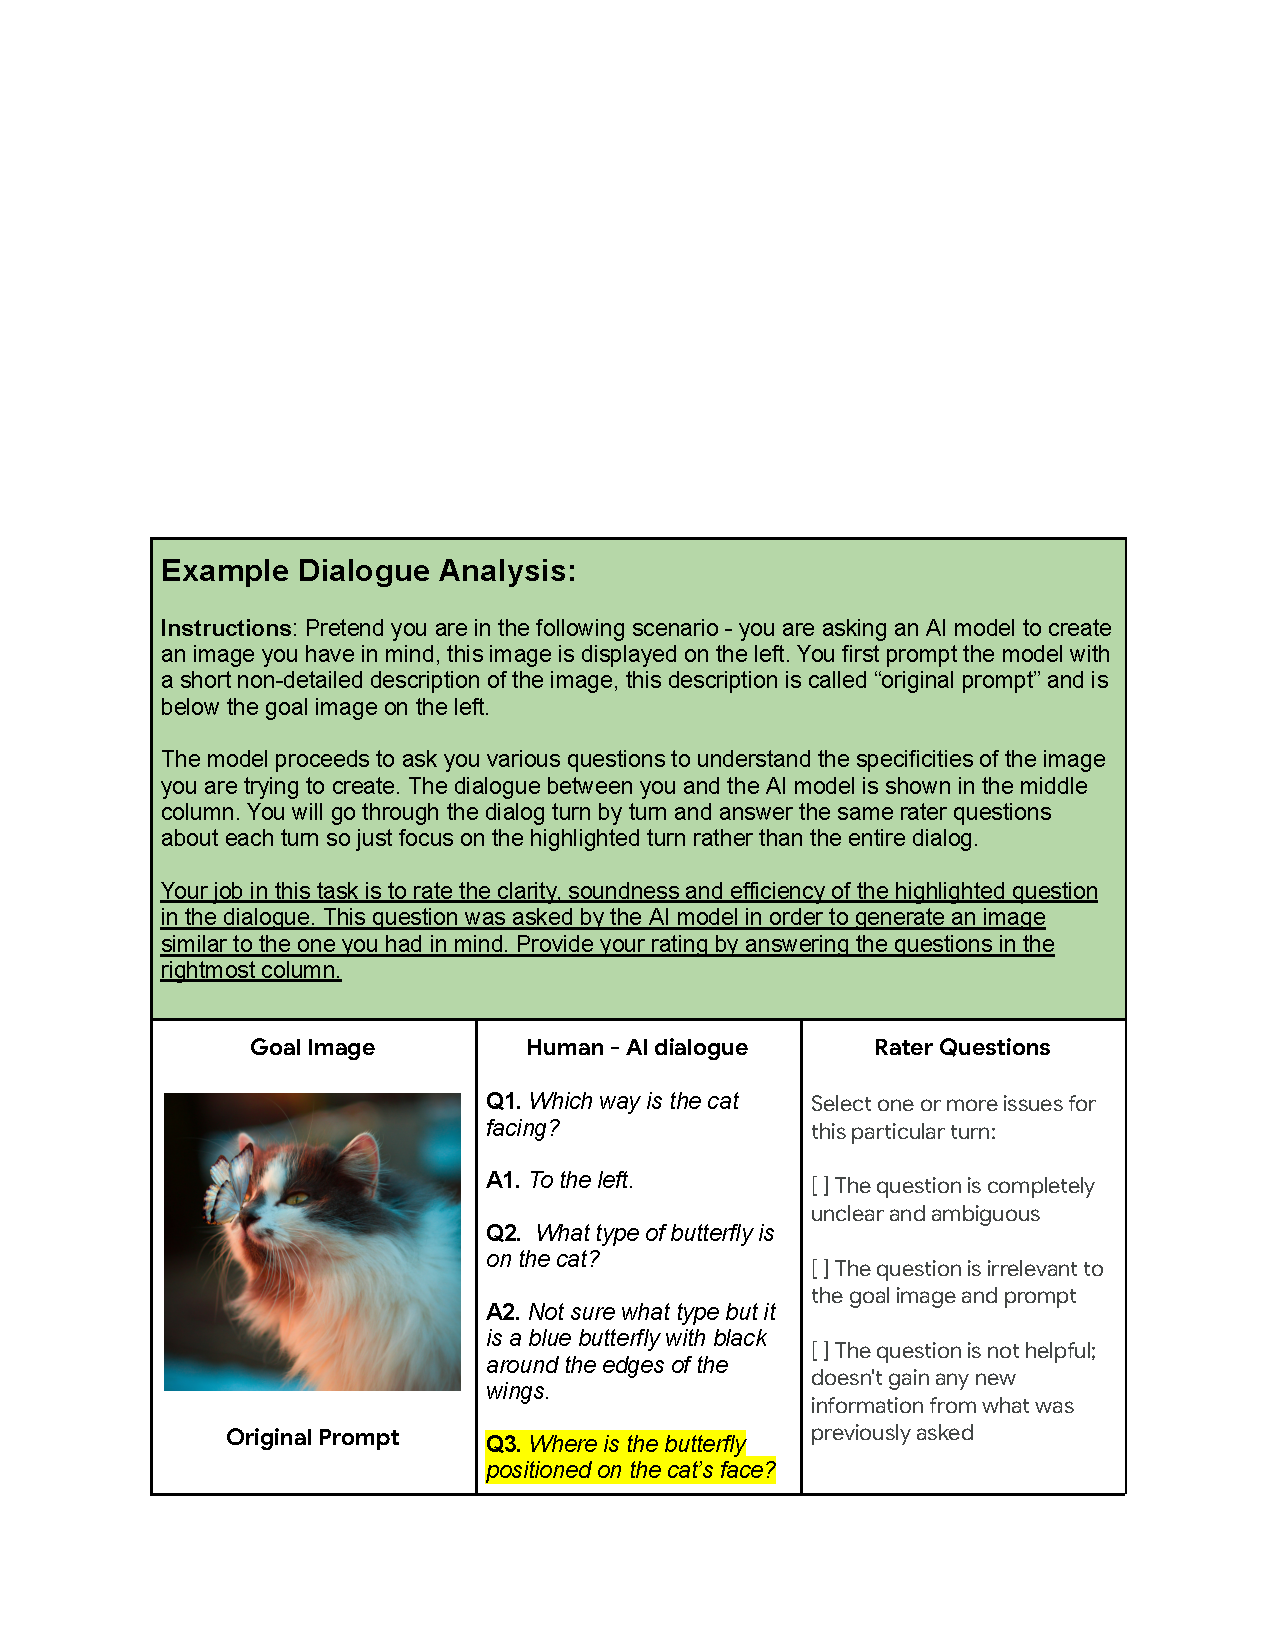
\includegraphics[width=.9\linewidth]{figures/Task_1.pdf}
    \caption{An example of the template presented to human raters. Human raters are asked to mark any issues a question contains that could pose a disturbance to the user. Approximately 8k questions per Agent are rated. The results are shown in \Cref{fig:rating_human_dialog}.}
    \label{fig:interface-human-model-task-1}
\end{figure} 
\clearpage

\textbf{Template of Human Rater Task 2: Evaluation of Similarity between the generated image and the Human-AI dialog and the original prompt.} 
\begin{figure} [H]
    \centering
    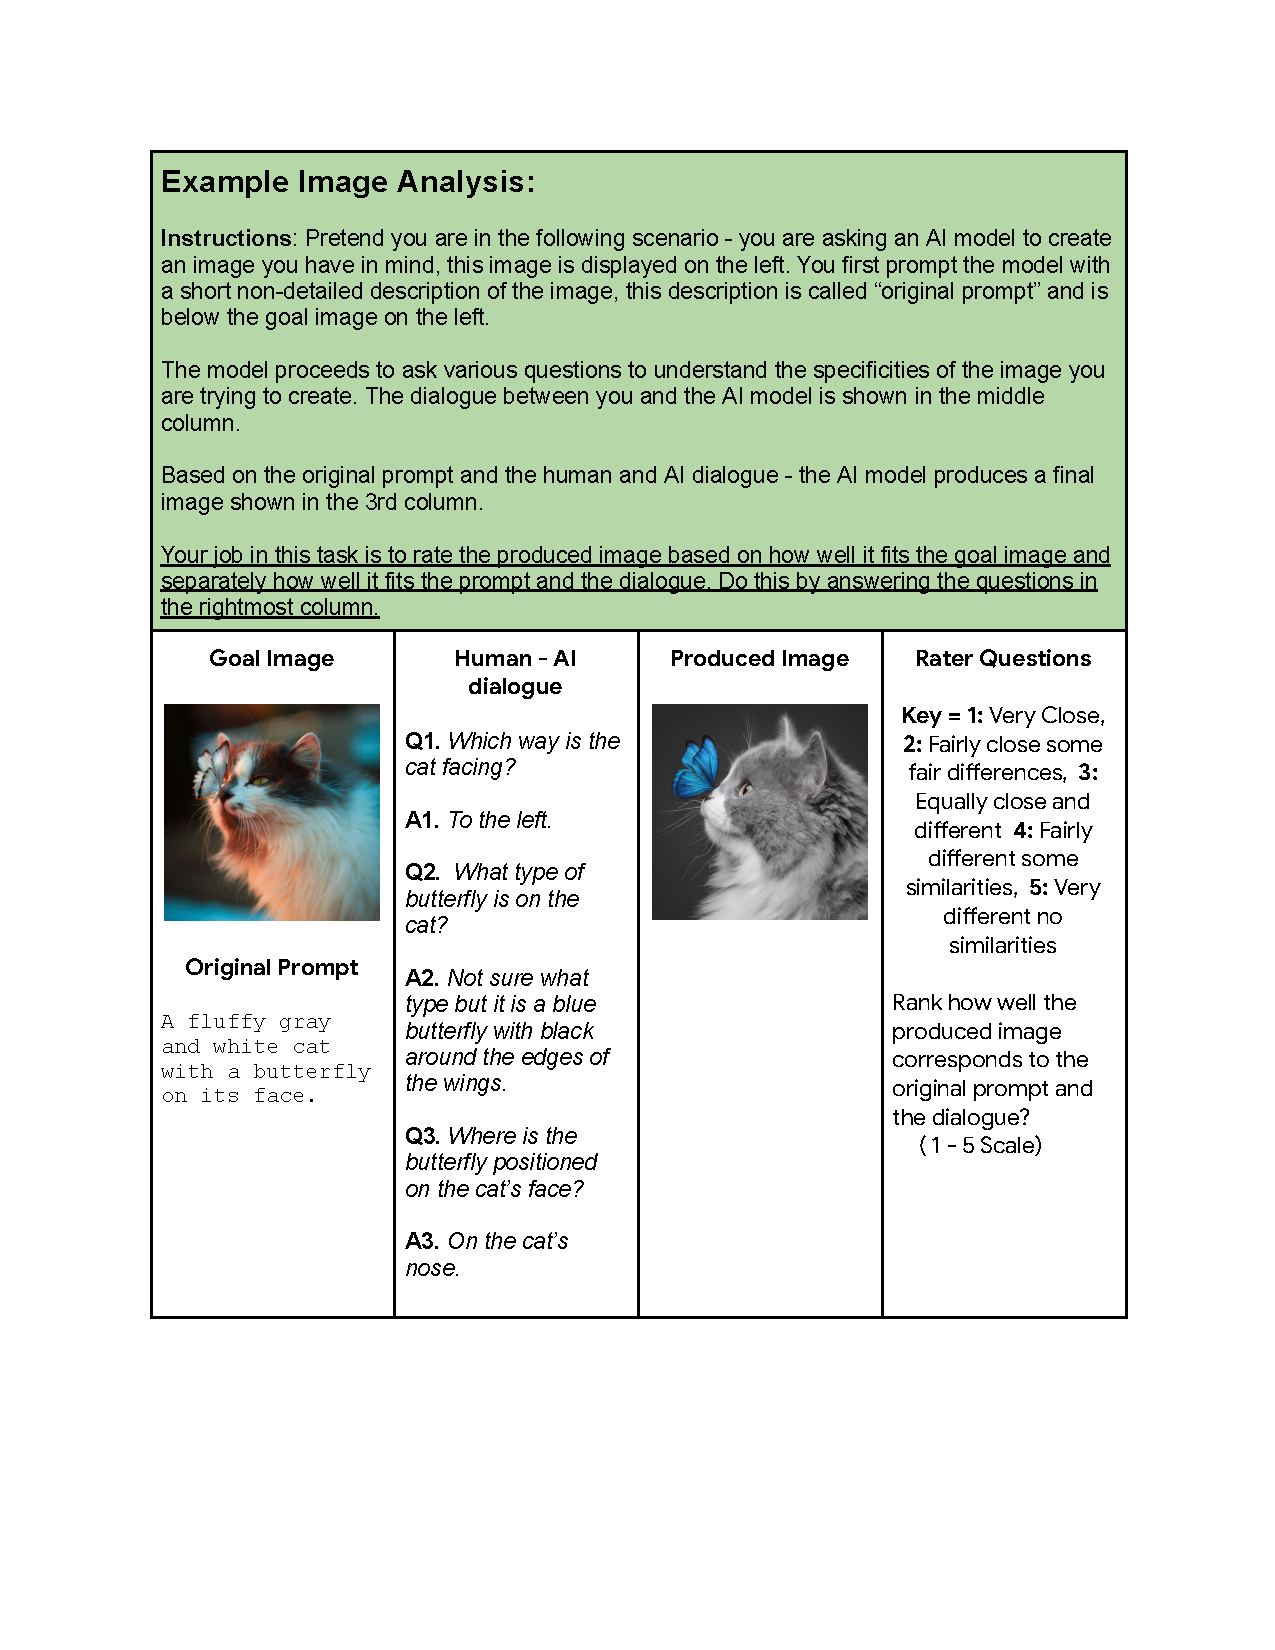
\includegraphics[width=.9\linewidth]{figures/Task_2.pdf}
    \caption{An example of the template presented to human raters. Human raters are asked to rank the correspondence of each image to the agent-user dialog and original prompt. Approximately 1.5k image-dialog pairs are rated using 3 human raters. Results in \Cref{fig:rating_human_dialog}.}
    \label{fig:interface-human-model-task-2}
\end{figure} 
\clearpage


\textbf{Template of Human Rater Task 3: Evaluation of the generated image similarity to the goal image.} 
\begin{figure} [H]
    \centering
    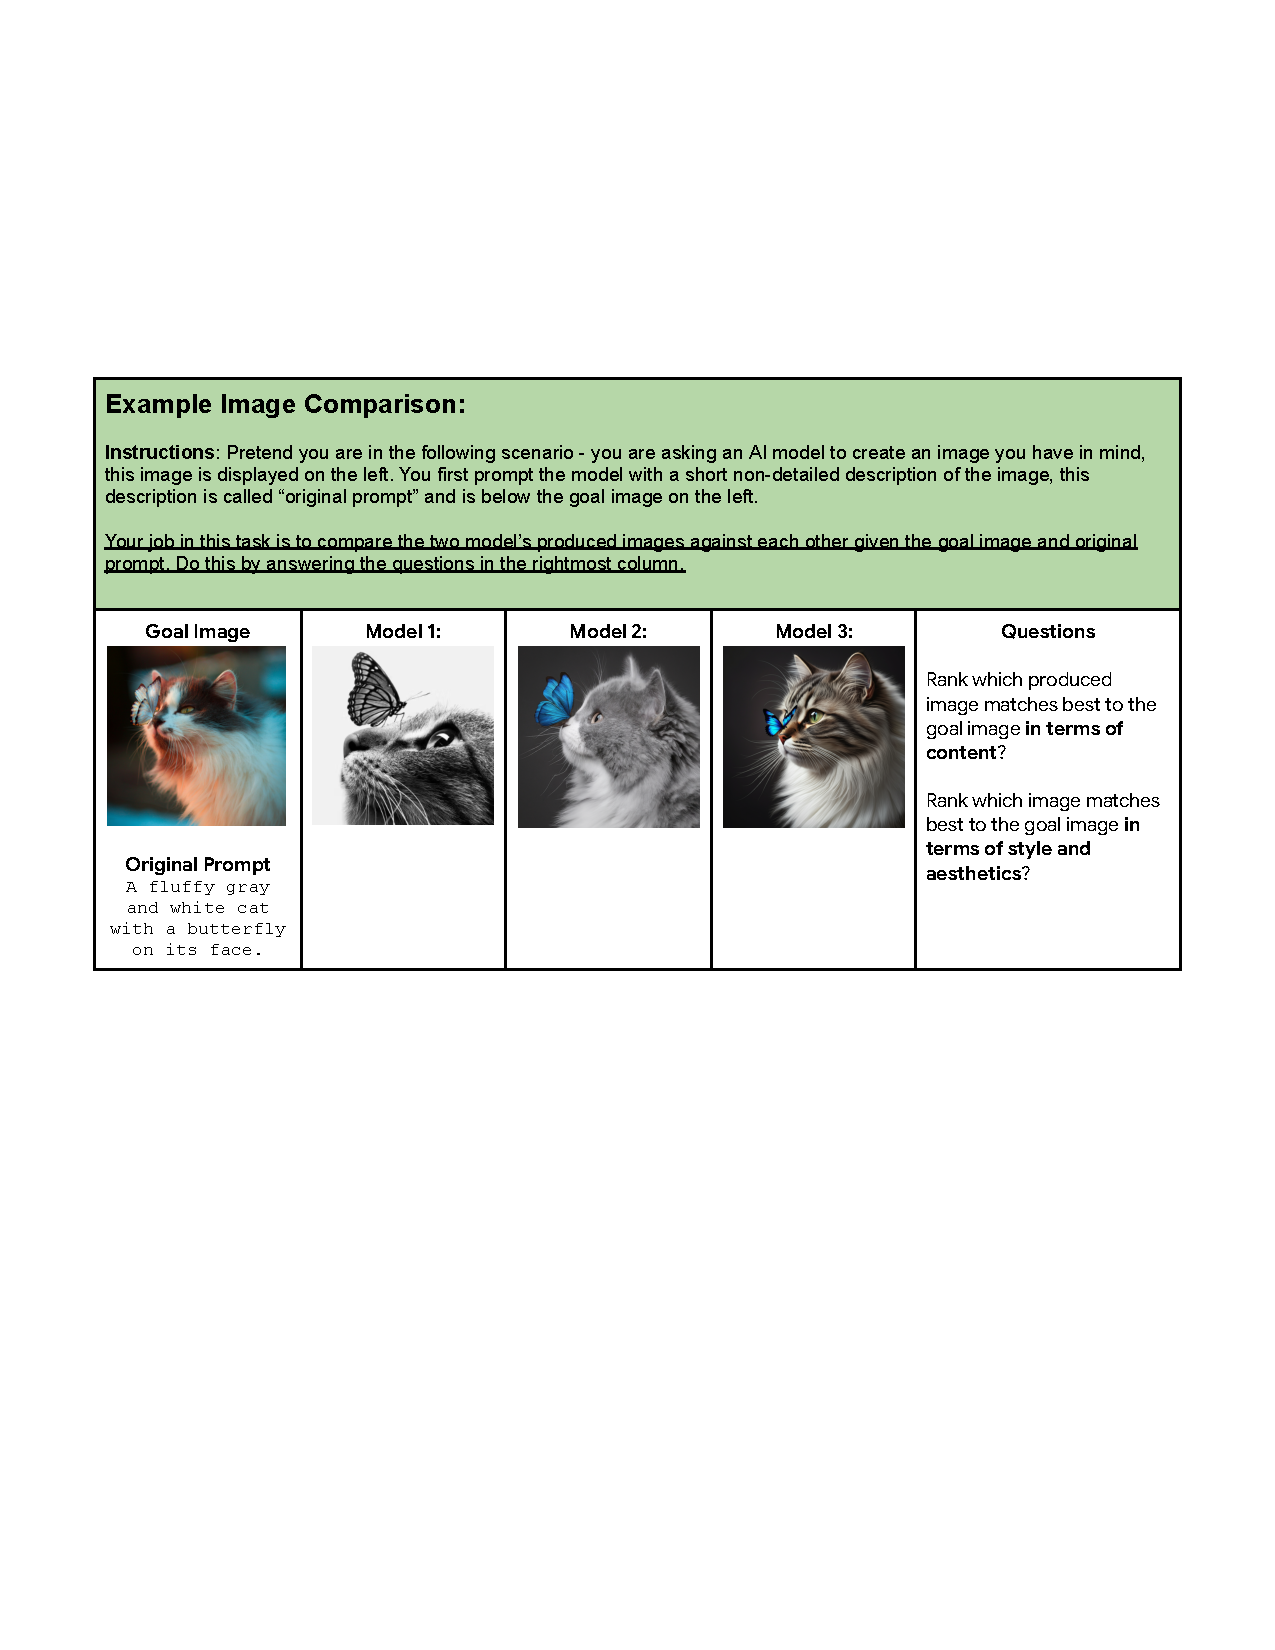
\includegraphics[width=.9\linewidth]{figures/Task_3.pdf}
    \caption{A template of the task presented to human raters. Human raters are asked to rate the images produced by the three proposed multi-turn agents and a single-turn T2I model against a Ground Truth image for which the original prompt was derived and the answers to the agents questions were derived. Approximately 550 image-dialog pairs per agent are rated using 3 human raters. The generated images were presented in a random order and were unlabeled and the human rater was tasked with ranking the images from best to worst. The results from the study are shown in \Cref{fig:rating_human_rank}.}
    \label{fig:interface-human-model-task-3}
\end{figure} 


\end{document}
